\documentclass{book}
%\documentclass[8pt]{book}
\usepackage{fancyhdr, flafter, makeidx, float, times}
\usepackage[T1]{fontenc}
\usepackage{graphicx}
\usepackage{fancyvrb}
\usepackage{listings}
\usepackage{varioref}
\usepackage[color]{ods}
\pagestyle{fancy}

%\addtolength{\headwidth}{\marginparsep}
%\addtolength{\headwidth}{\marginparwidth}
%       remember chapter title
%\renewcommand{\chaptermark}[1]%
%                  {\markboth{#1}{}}
%       section number and title
%\renewcommand{\sectionmark}[1]%
%              {\markright{\thesection\ #1}}
%\lhead[\fancyplain{}{\bfseries\thepage}]%
%      {\fancyplain{}{\bfseries\rightmark}}
%\rhead[\fancyplain{}{\bfseries\leftmark}]%
%      {\fancyplain{}{\bfseries\thepage}}
%\cfoot{}

%\setlength{\paperheight}{9in}
%\setlength{\paperwidth}{7.5in}
%\setlength{\textwidth}{5.5in}


%\floatstyle{ruled}
%\newfloat{code}{thp}{lop}[section]
%\floatname{code}{Code}
%\floatstyle{boxed}
%\newfloat{output}{thp}{lop}[section]
%\floatname{output}{Output}


%\DefineVerbatimEnvironment{code}{Verbatim}
%{commandchars=\\\#\?, tabsize=4, xleftmargin=1cm, 
% samepage=false, hfuzz=1pt, fontsize=\small,
% frame=lines, framesep=3mm}
%
%\DefineVerbatimEnvironment{codel}{Verbatim}
%{commandchars=\\\#\?, tabsize=4, xleftmargin=1cm, 
% samepage=false, hfuzz=1pt, fontsize=\small,
% frame=lines, framesep=3mm}

%\newenvironment{fvcode}[2]{\label{#1}
% \Verbatim[commandchars=\~\`\`, tabsize=4, xleftmargin=1cm, 
% samepage=false, hfuzz=1pt, fontsize=\small,
% frame=lines, framesep=3mm, label={Code \ref{#1}: \itshape{#2}}]}{\endVerbatim}

\lstdefinelanguage{tagsets}
 {morekeywords={trigger,do,else,done,if,while,when,break, breakif,
                set,unset,open,close,eval,cmp,exists,any,contains,ODS,proc,run},
  morekeywords=[2]{Define,End,start,finish},
  sensitive=false,
  morecomment=[s]{/*}{*/},
  morestring=[b]",
  morestring=[b]',
 }[keywords,comments,strings,directives]

\lstdefinestyle{tagsetstyle}
 {basicstyle=\small,
  stringstyle=\sffamily,
  keywordstyle=[2]{\bfseries\slshape},
  showspaces=false,
  showstringspaces=false,
  showtabs=false
  emphstyle=\underbar
 }

\lstdefinestyle{HTMLstyle}
 {language=HTML,
  basicstyle=\small,
  stringstyle=\sffamily,
  keywordstyle=[2]{\bfseries\slshape},
  showspaces=false,
  showstringspaces=false,
  showtabs=false
 }

\lstnewenvironment{fvcode}[2]
 {\lstset{label={#1}, caption={#2}, escapechar={~},
          frame=lines, xleftmargin=1cm, style=tagsetstyle}}
 {}

\lstnewenvironment{fvoutput}[2]
 {\lstset{label={#1}, caption={Output: #2}, frame=lines, xleftmargin=1cm, style=HTMLstyle}}
 {}

\lstnewenvironment{sfvcode}
 {\lstset{xleftmargin=1cm, style=tagsetstyle}}
 {}

\lstnewenvironment{sfvoutput}
 {\lstset{xleftmargin=1cm, style=HTMLstyle}}
 {}

\lstnewenvironment{poutput}[2]
 {\lstset{label={#1}, caption={Output: #2}, frame=single, xleftmargin=1cm, style=HTMLstyle}}
 {}

\newenvironment{goutput}[2]{\label{#1} \begin{figure} \caption{#2}}
  {\end{figure}}

\newenvironment{fvhtmcode}[2]{\label{#1}
 \Verbatim[commandchars=\\\{\}, tabsize=4, xleftmargin=1cm, 
 samepage=false, hfuzz=1pt, fontsize=\small,
 frame=lines, framesep=3mm, label={Code \ref{#1}: \itshape{#2}}]}{\endVerbatim}

\newenvironment{fvcodel}[2]{\label{#1}
 \Verbatim[commandchars=\~\`\`, tabsize=4, xleftmargin=1cm, 
 samepage=false, hfuzz=1pt, fontsize=\small,
 numbers=left, numbersep=5pt, 
 frame=lines, framesep=3mm, label={Code \ref{#1}: \itshape{#2}}]}{\endVerbatim}

\newcommand{\commandnames}[1]{\mbox{\large\textbf{#1}}\hfil}
\newcommand{\variablenames}[2]{\mbox{\large\textbf{#2}}\hfil}
\newcommand{\svariablenames}[2]{\mbox{\large\textbf{#2}}\hfil}
\newcommand{\commandargs}[1]{\normalsize\textit{#1}}
\newcommand{\tagsetalias}[1]{\index{#1}\normalsize\textit{Shortcut Alias: #1}}
%\newcommand{\commanditem}[2]{\entry{\commandnames{#1}\commandargs{#2}}}
\newcommand{\commanditem}[2]{\index{#1}\item[\commandnames{#1}]\commandargs{#2}}
\newcommand{\tagsetitem}[2]{\index{#1}\index{#2}\item[\commandnames{#1}]\tagsetalias{#2}}
\newcommand{\stagsetitem}[1]{\index{#1}\item[\commandnames{#1}]}
\newcommand{\variable}[2]{\item[\index{Variables!#1!#2}\variablenames{#1}{#2}]}
\newcommand{\stylevariable}[2]{\index{Variables!Style!#1!#2}\item[\svariablenames{#1}{#2}]}
\newenvironment{entry}
     {\begin{list}{}%
         {\renewcommand{\makelabel}{\commandnames}%
            \setlength{\labelwidth}{35pt}%
            \setlength{\leftmargin}{\labelwidth+\labelsep}%
         }%
     }%
     {\end{list}}


%\newenvironment{sfvcode}{
% \Verbatim[commandchars=\~\`\`, tabsize=4, xleftmargin=1cm, 
% samepage=false, hfuzz=1pt, fontsize=\small,
% frame=lines, framesep=3mm]}{\endVerbatim}

%\newenvironment{fvoutput}[2]{\label{#1}
% \Verbatim[commandchars=\~\`\`, tabsize=4, xleftmargin=1cm, 
% samepage=false, hfuzz=1pt, fontsize=\small,
% frame=lines, framesep=3mm, label={Output \ref{#1}: \itshape{#2}}]}{\endVerbatim}

%\newenvironment{sfvoutput}{
%\Verbatim[commandchars=\~\`\`, tabsize=4, xleftmargin=1cm, 
%samepage=false, hfuzz=1pt, fontsize=\small,
%frame=lines, framesep=3mm, label={\itshape Output}]}{\endVerbatim}

\newcounter{calloutcounter}[chapter]
\setcounter{calloutcounter}{1}
\newcommand{\calloutref}[1]{{\bfseries\ref{#1}}}
\newcommand{\callout}[1]{\label{#1}
 \refstepcounter{calloutcounter}
 \hspace{-5pt}
 {\bfseries 
  \thecalloutcounter
 \hspace{5pt}}
}

%  \marginpar[\flushright{\bfseries\value{calloutcounter}$\longrightarrow$}]
%             {{\bfseries $\longleftarrow$\value{calloutcounter}}}}

\newcommand{\calloutRepeat}{
 \hspace{-5pt}{\bfseries 
 \thecalloutcounter\hspace{5pt}}
}

%  \marginpar[\flushright{\bfseries\value{calloutcounter}$\longrightarrow$}]
%             {\bfseries$\longleftarrow$\value{calloutcounter}}}
% \hspace{-5pt}{\bfseries \value{calloutcounter}\hspace{0pt}}

\makeindex

%\includeonly{introduction, chapter1, chapter2,chapter3, chapter6, chapter7a, chapter4, chapter5, chapter5a, chapter4a, chapter7,chapter8,chapter9}

\begin{document}
\lstset{language=tagsets}
%\lstset{language=SAS}

% The way the preface titles are to be
\fancyhead{} %clear all fields
\fancyhead[LO,RE]{\thepage}
\fancyhead[RO]{}
\fancyhead[LE]{}
\fancyfoot[CO,CE]{}

\frontmatter
\title{ODS Markup: \\
Tagsets by Example}
\author{Eric Gebhart\\
SAS Institute}
\renewcommand{\today}{September 22, 2003}
\pagenumbering{roman}
\maketitle
  \section*{Preface}

The SAS Output Delivery System's (ODS) markup destination appears
to be much like all the other destination types that ODS is capable
of.  In reality it is quite different.  

The other ODS destinations have a
fixed output type.  The RTF destination can only create RTF output.
The printer destination can create postscript, PCL, and PDF.  But ODS
Markup can create any number of output types, all of which can be
created or modified by anyone.

ODS Markup is able to do this because it is really a framework which
uses a tagset to define what it should print to it's files.  The other
destinations, including the old HTML destination were hard coded
and compiled as a part of the SAS executable.  

A tagset can be described as a group of events or functions which use
a programming syntax similar to other programming languages such as
perl, python, shell, and datastep. 

We can create and use as many different tagsets as we like.  
There are a number of tagsets that come standard as a part of SAS.

Because there are so many different tagsets, ODS Markup is rather 
chameleon-like.  ODS HTML is really ODS Markup.  So is the CSV 
destination, and CHTML, excelXP, LaTeX, Troff, etc.  The only 
difference between these different ODS destinations is the tagset 
that is in use.  They are all really ODS Markup, we just don't call
it that.
 
When we use ODS Markup we are using a tagset.  The tagset determines
the type of output. Therefore, a tagset defines an output destination!
This realization has far reaching implications.  It means that we
can change the html that ODS HTML generates.  It means we can create
a new HTML destination with your corporate style and headings.  We
can create a new XML destination to allow data interchange with a
business partner or client. We can even create a simple flat file
format that can simplify processing by other programs. The output
can be modified and adapted in ways that could only be imagined until now.
The possiblities are endless.

It stands to reason, that if we want to use ODS Markup to our best
advantage, what we really want to do is use tagsets.  That
is what this book is going to explore.  What are these tagsets and how
do we use them?  You will find that tagsets can simplify otherwise
complex problems in a way that allows reuse and flexibility that
would not be possible with out them.

\cleardoublepage
\tableofcontents
\cleardoublepage
%\listoflistings
\cleardoublepage
\listoftables

%\listof{code}
%\listof{output}
% -----------------------document body

\mainmatter
\cleardoublepage
\pagenumbering{arabic}
\fancyhead{} %clear all fields
%\setlength{\headrulewidth}{1pt}
\lhead[\rm\thepage]{\sl\rightmark}
\rhead[\sl\leftmark]{\rm\thepage}

%The old fancyhead way.
%\fancyhead[LE,RO]{\thepage}
%\fancyhead[RE]{\bfseries Chapter \thechapter. \chaptermark}
%\fancyhead[LO]{\bfseries Section \thesection \sectionmark}
%\fancyfoot[CO,CE]{}

\part{Using ODS Markup and Tagsets}
%{
%These chapters will cover the basics of the ods markup statement,
%proc template, and tagsets.  The most commonly used tagsets will
% be explored and used.
%}

\cleardoublepage
\chapter{Introduction}
ODS markup and tagsets are the best way to create markup output
from SAS.  This book is divided into sections that will enable
you to get the most out of ODS Markup and Tagsets.  The first
section shows how ODS Markup and Tagsets are used.  Using an
ODS destination that is defined by a tagset is no harder than
using any other destination.  The most popular ODS Markup 
destinations are covered in this first section.

The next sections dig deeper into how Tagsets work and what
you can do to modify them or create your own.  This may
seem daunting at first, but frequently it is quite easy to
get Tagsets to do exactly what you want, saving lots of time
and effort further down a project's path.


\cleardoublepage
\chapter{The basics}
This chapter will cover the basics of using ODS Markup family of destinations.
There are a lot of ODS destinations in this family, and they are ready to
use.  By the end of this chapter you will have some idea of the destinations 
available, and how to use them.

ODS Markup is just another ODS destination that works very much
like every other ODS destination.  It was originally derived from
the original ODS HTML destination, so if you are familiar with ODS HTML,
then you are already very familiar with ODS Markup.

The way ODS Markup differs is that we will almost never use ODS Markup as
a destination name.  ODS Markup should be thought of as a family of destinations.
These destinations are defined using a type of template called Tagsets.  Each
Tagset definition is a new ODS destination.
 
The good news is that there are already a lot of Tagsets defined, so all we need
to do is use them.  Since Tagsets define destinations within the ODS Markup family
the only thing we really need to know is their names.  Once we know the tagset's 
name we know the destination name, and we can easily construct an ODS statement
that will use that ODS destination.



\section{It's all in the Name}
\index{basics}
\index{proc template}
\index{itemstore}
\index{sasuser}
\index{sashelp}
A tagset is a SAS program that uses Proc Template.  There are a lot of advantages to
this.  It means that SAS can update a tagset, make a fix, and even email that tagset
to anyone that wants it.  Updates to the Tagsets that shipped with SAS are available
for download on the Support.sas.com website.  Frequently there are also additional 
tagsets that were not shipped with SAS.  Another benefit, is that if you want to learn
to program Tagsets, you can create your own, or modify the Tagsets provided by SAS.

For now, the most important thing to know, is what are the Tagsets available, and 
what are they named.  All we really need is their names.  But where do we look?
When a Tagset is run in SAS, Proc Template compiles the Tagset and stores it
When a Tagset is run in SAS, Proc Template the Tagset
it into a binary format which is then stored on disk in an itemstore.
Typically this file will be in sasuser.  But can be placed anywhere
using the 'ODS path' statement.  If administrative priviledges are
available the template can be put in SASHELP where it will be
available to all users on the system.  Once a template is compiled
there is no need to compile it again unless it's itemstore is
deleted.  All Tagsets that ship with SAS are in SASHELP.

Thankfully, Proc Template handles all of this for us, and will look for Tagsets
in all the right places.  All we need is 3 lines of SAS code, and we will have
all the names for all the Tagsets.


\subsection{The tagset directory}
Templates are kept in directories within the itemstore.  ODS will automatically look for 
tagsets in the tagsets directory.  The following example shows how to get a list
of tagsets, and the output it generates.

\begin{fvcode}{list_tagsets}{Simple ODS Markup Statement}
       proc template;
           list tagsets;

                               The SAS System                               1
                                                  13:00 Monday, August 7, 2006

                Listing of: SASHELP.TMPLMST
                Path Filter is: Tagsets
                Sort by: PATH/ASCENDING
 
                Obs    Path                             Type
                 1     Tagsets                          Dir   
                 2     Tagsets.Cascading_stylesheet     Tagset
                 3     Tagsets.Chtml                    Tagset
                 4     Tagsets.Colorlatex               Tagset
                 5     Tagsets.Config_debug             Tagset
                 6     Tagsets.Csv                      Tagset
                 7     Tagsets.Csvall                   Tagset
                 8     Tagsets.Csvbyline                Tagset
                 9     Tagsets.Default                  Tagset
                10     Tagsets.Docbook                  Tagset
                11     Tagsets.Event_map                Tagset
                12     Tagsets.ExcelXP                  Tagset
                13     Tagsets.Graph_rtf                Tagset
                14     Tagsets.Html4                    Tagset
                15     Tagsets.Htmlcss                  Tagset
                16     Tagsets.Htmlpanel                Tagset
                17     Tagsets.Imode                    Tagset
                18     Tagsets.Latex                    Tagset
                19     Tagsets.MSOffice2k               Tagset
                20     Tagsets.Mlatex                   Tagset
                21     Tagsets.Mvshtml                  Tagset
                22     Tagsets.Namedhtml                Tagset
                23     Tagsets.Odsapp                   Tagset
                24     Tagsets.Odsgraph                 Tagset
                25     Tagsets.Odsstyle                 Tagset
                26     Tagsets.Odsxrpcs                 Tagset
                27     Tagsets.OpenOffice_rtf           Tagset
                28     Tagsets.Phtml                    Tagset
                29     Tagsets.Pyx                      Tagset
                30     Tagsets.Rtf                      Tagset
                31     Tagsets.Rtf_sample               Tagset
                32     Tagsets.SASReport11              Tagset
                33     Tagsets.SASReport12              Tagset
                34     Tagsets.SASReport13              Tagset
                35     Tagsets.SASReport14              Tagset
                36     Tagsets.SASReport15              Tagset
                37     Tagsets.SASReport_html           Tagset
                38     Tagsets.SASReport_html1          Tagset
                39     Tagsets.Sasreport_html11         Tagset
                40     Tagsets.Short_map                Tagset
                41     Tagsets.Simplelatex              Tagset
                42     Tagsets.Style_display            Tagset
                43     Tagsets.Style_popup              Tagset
                44     Tagsets.Supermap                 Tagset
                45     Tagsets.Tablesonlylatex          Tagset
                46     Tagsets.Text_map                 Tagset
                47     Tagsets.Tpl_style_list           Tagset
                48     Tagsets.Tpl_style_map            Tagset
                49     Tagsets.Troff                    Tagset
                50     Tagsets.Wml                      Tagset
                51     Tagsets.Wmlolist                 Tagset
                52     Tagsets.Xbrl                     Tagset
                53     Tagsets.Xhtml                    Tagset
       run;

NOTE: PROCEDURE TEMPLATE used (Total process time):
      real time           1:40.15
      cpu time            0.28 seconds
      
\end{fvcode}

\section{Using a tagset}
That is a lot of Tagsets!  For now, lets concentrate on the obvious
ones.  
To use a tagset, all that is needed is the proper ods statement.
ODS Markup is not all that different from ODS HTML, in fact, ODS
Markup can do everything ODS HTML can, plus a little more.
The simplest form of the ODS Markup statement is shown 
in Figure \ref{ods_markup_stmt} on page \pageref{ods_markup_stmt}.

\index{ods statement}
\begin{fvcode}{ods_markup_stmt}{Simple ODS Markup Statement}
   
    ods markup file='test.xml';

    ....

    ods markup close;

\end{fvcode}

\index{ods markup statement}
\index{tagsets.default}

The result of those statements will be the creation of the 'test.xml' output
file.  The output of that file will have a format as defined by the default
tagset, which is named, tagsets.default.

But there are other ways to specify an ODS statement that accomplish the same thing.
Figure \ref{ods_markup_stmt_perm} on page \pageref{ods_markup_stmt_perm}.
shows ods statements which are equivalent with one exception.

\begin{fvcode}{ods_markup_stmt_perm}{ODS Markup Statement Permutations}
\index{ods markup statement!permutations}

    ods markup file='test.xml';

    ods markup tagset=default file='test2.xml';

    ods tagsets.default file='test3.xml';

\end{fvcode}

The exception is the third statement.  That statement is different because the destination
name is no longer markup.  The destination name is tagsets.default.   Because it has a
unique name it can run simultaneously with ods markup.  Just like ODS RTF can run simultaneously
with ODS HTML.  The first two statements cannot be used simultaneously because they have the
same destination name.  The second ODS Markup 
statement would automatically close the first one.  This happens because ODS destination names
must be unique.  There is a way around that, using ODS' ID syntax, but that belongs in another
book.  Beside's that syntax is mostly uneccessary if we use the tagset name as the destination
name, and the resulting code is more readable and concise.


As of SAS 9.1, ODS HTML is also a tagset.  Which means ODS HTML is really ODS Markup.  Consider
the statements in figure \ref{ods_markup_stmt_perm2} on page \pageref{ods_markup_stmt_perm2}.

\index{ods markup statement!permutations}
\begin{fvcode}{ods_markup_stmt_perm2}{ODS Markup Statement Permutations}
    ods html file='test1.html';

    ods html4 file='test2.html';

    ods tagsets.html4 file='test3.html';

    ods markup tagset=html4 file='test4.html'
\end{fvcode}

Each one of those statements is roughly equivalent.  All of them use the html4 tagset.  So
the markup each of them creates will be the same.  But each ODS statement creates a unique
output destination.  They can all run simultaneously without conflict.  They can all have their
own select or exclude statements and be opened or closed at different times.   

There is one thing that makes html special.  Normally a tagset cannot be referenced by
it's simple name unless the tagset option is used. But there are a few special tagsets that
can be referenced as if they are a simple ODS destination.  
Table \ref{shortcut_destinations} on page \pageref{shortcut_destinations} shows the list
of shortcut names and their descriptions.


\index{Simple names}
\index{Shortcut destinations}
\begin{table}\caption{Shortcut Destination names}
\label{shortcut_destinations}
\begin{tabular}{l|l}
%\multicolumn{2}{c}{Shortcut Destinations} \\ 
\hline
HTML &  Alias for HTML4 \\
HTML4 & 4.0 compliant HTML with concessions for browser compatibility. \\
PHTML & Plain HTML.  Simple stylesheet, simple HTML. \\
HTMLCSS & 4.0 compliant HTML with fewer concessions. \\
CSV &  Comma separated values.  Tables only. \\
CSVAll & CSV with titles, bylines, notes, etc. \\
CSVByline & CSV with bylines only. \\
WML &  Wireless Markup Language. - No longer in vogue. \\
CHTML & Compact HTML. Very simple HTML with no styles. \\
LaTeX & LaTeX output with style and color support. \\
Troff & troff output which is very simple. \\
MSOffice2K & HTML for importing into Word and Excel. \\
Imode & Compact HTML that has no table tags.  Used extensively in Japan. \\
DocBook &  XML format for documents. \\
SasReport & XML format used internally by other SAS products.
\end{tabular}
\end{table}

While these are special, the custom tagsets that can be written are no less special.  These
custom tagsets cannot be referenced by their simple names but they will be output destinations just
as these are.  Because Markup is a single destination, the prefered way to use tagsets is to
use their two part name.  There is a trend away from using these shortcut names, so most of the
newer tagsets like ExcelXP and RTF can only be referenced by their full name.
See Figure \ref{ods_markup_stmt_active} on page \pageref{ods_markup_stmt_active} shows the list

\index{ods markup statement!permutations}
\index{ods markup statement!Multiple Active}
\begin{fvcode}{ods_markup_stmt_active}{Multiple Active Markup Destinations}

    ods tagsets.ExcelXP file='test.xml';
    ods tagsets.RTF file='test.rtf';

    proc print data=sashelp.class; 
    run;

    ods tagsets.ExcelXP close;
    ods tagsets.RTF close;

\end{fvcode}
     
\section{Summary}
Using ODS Markup does not have to be complicated or difficult, all we really
need is the name of the Tagset, and we can use them just like any other destination.
Finding their names is very simple Proc Template code, and adding an ods statement that uses them is
just as easy.  It won't hurt anything to try out a destination just to see what it
will create.  Go ahead, play, try them out.  The next chapters will go into more 
detail for many of the more popular and useful Tagsets that are available.

The most confusing thing about the ods markup statement is that it
is almost never used by it's name.  Aside from that it is almost
the same as any other ods destination, especially the ODS HTML
destination in previous releases of SAS.


\cleardoublepage
\chapter{Using The CSV Destinations.}
The CSV Tagsets are some of the most useful tagsets around,
the format has been used for decades by various applications
and everyone knows what to expect from a CSV file.  This chapter
will explain how to use the 3 different CSV tagsets provided by SAS.

\index{CSV}
\index{Excel!CSV}
\index{Excel!Live Data}
Comma separated values are one of the simplest formats that are
is understood by many different applications.  The disadvantage is that
there is no formatting, fonts, or colors.  Still CSV files work
very well for many applications.  A CSV file can be connected as
live data to an Excel Template.  This can be a convenient way to
publish Excel spreadsheets to many people.  

\index{CSV|Tagsets}
\index{CSV|CSVALL}
\index{CSV|CSVBYLINE}
There are three different CSV Tagsets shipped with SAS.  The
simplest is the CSV Tagset, next comes CSVByline, and last
is CSVAll.  The CSV Tagset only creates output from tabular
data, there are no titles, footnotes, bylines, Notes, there
is nothing but tables.  It didn't take long to find out that
there were people who wanted titles and footnotes and everything
else, that's when CSVAll came into existence.  It also became
apparent that just having tables and bylines was a nice thing to
have, so CSVBylines was born.  All of these tagsets use the same
base Tagset to create the CSV data, so there is no other difference
in behavior besides the verbosity of the output.

Both CSV and CSVAll have aliases so that they can be referenced by
a simple name, rather than the full tagset name.  CSVByline has no
alias, so it must be used with it's full name.  Here are examples
of each of these ODS statements.

\begin{sfvcode}
ODS CSV file='test.csv';
ODS CSVAll file='testall.csv';
ODS tagsets.CSVByline file='testby.csv';
\end{sfvcode}

Using these statements around a simple Proc Print will show how
these destinations vary.

\begin{sfvcode}
ODS CSV file='test.csv';
ODS CSVAll file='testall.csv';
ODS tagsets.CSVByline file='testby.csv';

options obs=6;

proc sort data=sashelp.class out=sorted;
     by sex;

Proc print data=sorted;
     by sex;
run;

ODS _all_ close;
\end{sfvcode}

None of the output from this example is very complicated,
but each has it's differences.  The CSV Tagset ignores the title
and the bylines. But it does create the two tables as a result of
the by.

\begin{sfvoutput}
"Obs","Name","Age","Height","Weight"
"1","Alice",13,56.5,84.0
"2","Barbara",13,65.3,98.0
"3","Carol",14,62.8,102.5

"Obs","Name","Age","Height","Weight"
"4","Alfred",14,69.0,112.5
"5","Henry",14,63.5,102.5
"6","James",12,57.3,83.0
\end{sfvoutput}

The CSVByline Tagset adds the bylines, but nothing else.

\begin{sfvoutput}
"Sex=F"
"Obs","Name","Age","Height","Weight"
"1","Alice",13,56.5,84.0
"2","Barbara",13,65.3,98.0
"3","Carol",14,62.8,102.5

"Sex=M"
"Obs","Name","Age","Height","Weight"
"4","Alfred",14,69.0,112.5
"5","Henry",14,63.5,102.5
"6","James",12,57.3,83.0
\end{sfvoutput}

Finally, the CSVAll tagset adds in the title.  If there were
footnotes, or procedure titles, or any of the four flavors of
notes; Note, Warning, Error, or Fatal, those would be included as well.

\begin{sfvoutput}
The SAS System

"Sex=F"
"Obs","Name","Age","Height","Weight"
"1","Alice",13,56.5,84.0
"2","Barbara",13,65.3,98.0
"3","Carol",14,62.8,102.5

"Sex=M"
"Obs","Name","Age","Height","Weight"
"4","Alfred",14,69.0,112.5
"5","Henry",14,63.5,102.5
"6","James",12,57.3,83.0
\end{sfvoutput}

In the beginning it seemed that this was everything that any CSV tagset
would ever need to do.  But even the simplest of outputs is not always 
that simple.  Tagsets needed to be able to adapt to what was needed of them.
The best way to do that is to have the ability to give the tagset some variable
to help it make decisions on how to behave.  Up until SAS 9.1.3 the only way
to do that was with macro variables.  Macro variables still work, but now there
is a better way.  With SAS 9.1.3 the ODS Markup statement was given a new option,
the options(...) option.  Options are a nearly arbitrary set of key value pairs
that the tagset will recieve.  It is completely up to the Tagset to process those
values and use them. 

Surprisingly the CSV Tagset has quite a number of options. In fact everything
that the CSVAll and CSVByline tagsets do can be done by the base CSV Tagset.
In SAS 9.1.3 the only thing CSVALL and CSVByline Tagsets do is set up some new defaults for
the CSV options available.

With the proliferation of Tagset options it didn't take long to figure out we needed
another option, Help!  All Tagsets that have options have an option called doc.  The Doc
option is all you need to find out just what a Tagset can do.  Asking for help may be
the first thing you want to do when using a new tagset.  If there are options, Help will
tell you about them.  Help isn't in all of the Tagsets, but the number is growing and
it never hurts to ask.  Here is how we ask for help.

\begin{sfvcode}
ODS CSV file='test.csv' options(doc='help');
\end{sfvcode}

The output from help will go to the log and for CSV, it looks like this.

\begin{sfvoutput}
==============================================================================
The CSV Tagset Help Text.
 
This Tagset/Destination creates output in comma separated value format.
 
Numbers, Currency and percentages are correctly detected and show as numeric values.
Dollar signs, commas and percentages are stripped from numeric values by default.
 
==============================================================================
 
These are the options supported by this tagset.
 
Sample usage:
 
ods csv options(doc='Quick'); 
 
ods csv options(currency_as_number='yes' percentage_as_number='yes' delimiter=';'); 
 
Doc:  No default value.
     Help: Displays introductory text and options.
     Quick: Displays available options.
 
Delimiter:   Default Value ','
     Sets the delimiter for the values.  Comma is the default.  Semi-colon is
     a popular setting for european sites.
 
currency_as_number:   Default Value 'No'
     If 'Yes' currency values will not be quoted.
     The currency values are stripped of punctuation and currency symbols
     so they can be used as a number.
 
percentage\_as\_number:   Default Value 'No'
     If 'Yes' percentage values will not be quoted.
     The percentages are stripped of punctuation and the percent sign
     so they can be used as a number.
 
Currency\_symbol:   Default Value '\$'
     Used for detection of currency formats and for 
     removing those symbols so excel will like them.
     Will be deprecated in a future release when it is
     no longer needed.        
 
Decimal\_separator:   Default Value '.'
     The character used for the decimal point.
     Will be deprecated in a future release when it is no longer needed.
 
Prepend\_Equals:   Default Value 'no'
     Put an equal sign in front of quoted number values.
     This only works in conjunction with quote_by_type.
 
quote\_by\_type:   Default Value 'no'
     Put values based on the type, not based on what the regex match for number.
 
Table\_Headers:   Default Value 'yes'
     If no, skip the header section of all tables.
 
Thousands\_separator:   Default Value ','
     The character used for indicating thousands in numeric values.
     Used for removing those symbols from numerics so excel will like them.
     Will be deprecated in a future release when it is no longer needed.
 
Quoted\_columns:   Default Value ''
     A list of column numbers that indicate which values should be quoted
     ie. Quoted\_columns="123"
 
Empty\_Missing:   Default Value 'no'
     If yes, missing values will not show in any way other than positionally.
 
Bylines:   Default Value: No
     If yes bylines will be printed
 
Titles:   Default Value: No
     If yes titles and footnotes will be printed
 
Notes:   Default Value: No
     If yes Note, Warning, Error, and Fatal notes will be printed
 
Proc\_Titles:   Default Value: No
     If yes titles generated by the procedures will be printed
 
\end{sfvoutput}


The help you get will depend upon which version of the tagset you have.
There are the expected options that reflect the behaviors we have seen
from the CSVAll and CSVByline Tagsets, but there is much more.  One
of the most used options is Delimiter, this makes it easy to change the
field delimiter to a ;, a | or even tabs.  Another thing that became
obvious was that there needed to be a way to detect numbers in any one
of the various European formats.  That's where decimal\_separator, thousands\_separator
and currency\_symbol come in.  Not everyone uses a '.' for decimals, or ',' for
thousands. 

There are a few less obvious options in there.  Table\_headers turns the table\_headers
on and off.  Empty\_missing makes missing values go completely away, with just it's
field delimiters showing where it would have been.  

Currency\_as\_Number, and Percentage\_as\_Number,
are there because not everyone wants those values as strings, So if you want them as numbers,
these options will do that for you, they will also strip out any symbols that would prevent
Excel from seeing those values as numbers.

Another option that is just for excel, is prepend\_equals, this option will put an '=' in front
of quoted numbers so that Excel will read the value correctly, even if it has leading zeros.  So
if you have leading zero's this is the option you want.

The last two have to do with quoting.  Currently, the CSV tagset tries it's best to figure out
what is a string and what is a number.  It doesn't always do exactly what we want.  Part of
the problem is that some procedures don't tell the Tagset what is what.  Proc Print is one of
those procedures that does say which value is a string and which is a number.  The quote\_by\_type
option tells the tagset to stop guessing and do what Proc Print or any other proc says.  The
exception to this, until SAS 9.2, is Proc Report, and Proc Tabulate.  Those are the two Procs
that don't give the tagset any clues.

To further extend the ability to control quoting, There is a Quoted\_columns option that will
allow for columns to be specified by number.  So if all else fails and you still can't get
your values quoted where you want, this option should do the trick.


By default the csv tagset only displays tables.  Turning on bylines so that it looks
like the output from the CSVByline Tagset 
is just a matter of setting the bylines option to yes.  Changing the Delimiter to a
';' is just as easy.  Of course we could have used the CSVByline Tagset with just
the delimiter option to do the same thing.

\begin{sfvcode}
ODS CSV file='test.csv' options(delimiter=';' bylines='yes');
ODS tagsets.CSVByline file='test.csv' options(delimiter=';');

options obs=6;

proc sort data=sashelp.class out=sorted;
     by sex;

Proc print data=sorted;
     by sex;
run;

ODS _all_ close;
\end{sfvcode}

The output from both of these ODS statements looks identical.

\begin{sfvoutput}
"Sex=F"
"Obs";"Name";"Age";"Height";"Weight"
"1";"Alice";13;56.5;84.0
"2";"Barbara";13;65.3;98.0
"3";"Carol";14;62.8;102.5

"Sex=M"
"Obs";"Name";"Age";"Height";"Weight"
"4";"Alfred";14;69.0;112.5
"5";"Henry";14;63.5;102.5
"6";"James";12;57.3;83.0
\end{sfvoutput}

Knowing how the CSVByline and CSVAll Tagsets work can be quite handy, Especially
if you find that you always want the same basic set of options.  It is much easier
to create your own Tagset than it is to always type in the same options over and over.
Here is the entire code for the CSVByline Tagset.  Before you look, realize that most
of this is copied and pasted from the CSV Tagset.

\begin{sfvcode}
   define tagset tagsets.csvbyline;
       parent=tagsets.csv;

        define event initialize;
            set \$options['BYLINES'] 'yes';
            trigger set_options;
            trigger documentation;
            trigger compile_regexp;
        end;
    end;
\end{sfvcode}

The only addition to the copied and pasted code is this line.

\begin{sfvcode}
            set \$options['BYLINES'] 'yes';
\end{sfvcode}

We can take advantage of this knowledge and create our own CSV Tagset that
has it's own set of default option values.  If we want the same behavior from
the new Tagset as 
our previous example a new name is probably in order.  After all it's no longer
comma separted values, it's semi-colon separated values. 
Our new Tagset would look like this.  Be aware that option
names are always capitalized inside the tagset.

\begin{sfvcode}
proc template;
   define tagset tagsets.ssvbyline;
       parent=tagsets.csv;

        define event initialize;
            set \$options['BYLINES'] 'yes';
            set \$options['DELIMITER'] ';';
            trigger set_options;
            trigger documentation;
            trigger compile_regexp;
        end;
    end;
run;
\end{sfvcode}

All we have to do is run that Proc Template, and our new tagset is ready to use.
Congratulations! You've just written your first Tagset!  If someone else wants 
output that has bylines and semi-colons for field separators, just tell them to
do this!

\begin{sfvcode}
     ODS tagsets.ssvbyline file='test.csv' options(doc='help');
\end{sfvcode}

The output looks exactly like the output above.  It is, after all, generated the same way.

\section{Summary}
The CSV destinations are very easy to use and although the output is very simple, there are
many options that can be used to control how that output is created.  ODS Markup options 
provide a very versatile way to change the behavior of any Tagset destination.  Finding out
what those options are, and how to use them is as easy as asking for help.  Add options(doc='help')
to any ODS Markup/tagsets statement and find out just what that Tagset can do for you.
Creating a new Tagset that sets the options just the way you want is almost as easy is copy
and paste.    
That's what tagsets are all about, creating output just the way you want it,
in a reusable and easy way.







\cleardoublepage
\chapter{Using The HTML Tagsets}
\index{Tagsets!HTML}
\index{Destinations!HTML}
HTML is certainly one the most popular output typs available.
Not only is easily used to report information on the web, but it
is also a commonly understood import format for many applications.
ODS Markup has several HTML tagsets to choose from when it comes
to creating HTML output.  Each of these Tagsets has some advantage
in one way or another depending upon how it will be used.
This chapter will explain the different HTML tagsets and the
features they support.


\section{The Different HTML's}
\index{Destinations!HTML}
ODS HTML is one of the aliased destination names that really 
means use the tagsets.html4 Tagset.  Someday it may well mean
use the Tagsets.html5 Tagset.  But that is in the future.

There are several other aliases, for the various HTML tagsets.
PHTML, HTMLCSS, CHTML and CHTML\_imode are the 
other shortcut names for HTML tagsets.  These aliases map directly
to their tagset names, the aliases just keep us from having to put 'tagsets.'
in front of them.

Only one example is needed in order to
see the major differences between the different HTML tagsets available.
There are differences in style, the way titles and footnotes are processed,
and in the case of the MSOffice2k tagset, there is a difference in how the
tables are rendered.  All that is needed to see this differences is a 
couple of title statements and some simple Proc Tabulate output.

This example has three titles, the default title, and two more titles that
use the 3 part title syntax.  It is the use of style and 3 part titles that
will show major differences between these various HTML destinations.  

\begin{sfvcode}
ods html file="html.html";
ods xhtml file="xhtml.html";
ods htmlcss file="htmlcss.html";
ods phtml file="phtml.html";
ods tagsets.MSOffice2K file="msoffice2k.html";
ods chtml file="chtml.html";
ods imode file="imode.html";


  title3 height=15pt color=orange
         justify=right '15 pt first right'
         justify=left 'first left';
  title4 height=10pt color=red 'no justify red'
         justify=right 'Second right'
         justify=left 'Second left';

proc sort data=sashelp.class out=work.class;
    by age  sex;
run;

options obs=2;

PROC TABULATE DATA=class;
   VAR Height Weight;
   CLASS Sex Age;
   TABLE Age*Mean ALL*Sex*Mean,
         Weight;
   by age;
   
RUN;

ods _all_ close;
\end{sfvcode}


\subsection{HTML4 And XHTML}
\index{Destinations!HTML}
\index{Destinations!HTML4}
\index{Destinations!HTML3}
\index{Destinations!XHTML}
HTML4 and HTML are really the same thing and XHTML is nearly the same but not quite.
The only thing the XHTML tagset does is add XML compliant tags to the HTML.
If you don't know what that is, don't worry about it.  For all practical purposes
they are nearly identical.

The HTML destination does not have to be HTML4, it could be set to be HTML3.
There is a registry setting
that will allow HTML to be the legacy version HTML.  HTML3 is
the name of what was the HTML destination in SAS 8.2.  HTML3 does
not use tagsets or ODS Markup at all.  It is done the old fashioned way
with C-code.  HTML3 has remained virtually unchanged since SAS 8.2.

Let's look at the HTML4 output first since HTML4 is the tagset that does everything.
There aren't any surprises here.  It looks just the way we would expect.
The titles are colored, and justified on the page just the way they should be.

IMAGE MISSING....
%\includegraphics[width=6in]{html.html.png}

Use this output as a reference as you look at the output for the rest of these HTML
destinations.  It will give you a good idea of how they all behave.

\subsection{HTMLCSS}
\index{Destinations!HTMLCSS}
\index{HTMLCSS}
HTMLCSS is a basic stylesheet based HTML tagset.  There is very little difference
between the HTML4 tagset and HTMLCSS. Both the HTML4 and MSOffice2k tagsets inherit
most of their events from the HTMLCSS tagset, and ultimately the PHTML tagset.


\subsection{PHTML}
\index{Destinations!PHTML}
\index{PHTML}
The PHTML tagset generates a very plain HTML.  The huge stylesheet is replaced
by a much smaller stylesheet.  If you dislike all the styles and the verbosity
of the html4 and htmlcss tagsets then this tagset is a good place to start.


\subsection{XHTML}
\index{Destinations!XHTML}
\index{XHTML}
The XHTML tagsets is one of the shortest tagsets around.  It inherits from the HTML4
tagset.  All it adds are the stricter XML style tags.

\subsection{MSOffice2K}
\index{Destinations!MSOffice2k}
\index{MSOffice2k}
The MSOffice2k tagset is a good tagset to use if you want to import the resulting HTML
into Microsoft Office.  This tagset adds Microsoft specific XML to the HTML so that 
Microsoft office can size images better.  It also creates different HTML for titles and
footnotes so that they import more smoothly into Excel.  This tagset also works with proc
tabulate to create a better array of table cells, so that Excel will keep all of the
rows straight.


\subsection{HTML4}
\index{Destinations!HTML!Stylesheets}
The HTML tagsets that use styles always use a stylesheet, if no stylesheet file
is specified the stylesheet is still written to the top of the
body file.  Using an external stylesheet allows more flexibility
and it can allow multiple reports to use the same stylesheet file.

\begin{sfvcode}
   ODS html file='test.html';

   proc print data=sashelp.class; run;

   ODS html close;
\end{sfvcode}



\subsection{PHTML}
\index{Destinations!PHTML}
\index{PHTML}
The PHTML tagset generates a very plain HTML.  The huge stylesheet is replaced
by a much smaller stylesheet.  If you dislike all the styles and the verbosity
of the html4 and htmlcss tagsets then this tagset is a good place to start.


\subsection{HTMLCSS}
\index{Destinations!HTMLCSS}
\index{HTMLCSS}
HTMLCSS is a basic stylesheet based HTML tagset.  There is very little difference
between the HTML4 tagset and HTMLCSS. Both the HTML4 and MSOffice2k tagsets inherit
most of their events from the HTMLCSS tagset, and ultimately the PHTML tagset.

\subsection{XHTML}
\index{Destinations!XHTML}
\index{XHTML}
The XHTML tagsets is one of the shortest tagsets around.  It inherits from the HTML4
tagset.  All it adds are the stricter XML style tags.

\subsection{MSOffice2K}
\index{Destinations!MSOffice2k}
\index{MSOffice2k}
The MSOffice2k tagset is a good tagset to use if you want to import the resulting HTML
into Microsoft Office.  This tagset adds Microsoft specific XML to the HTML so that 
Microsoft office can size images better.  It also creates different HTML for titles and
footnotes so that they import more smoothly into Excel.  This tagset also works with proc
tabulate to create a better array of table cells, so that Excel will keep all of the
rows straight.

\section{HTML and Excel}
\index{Excel!HTML}
\index{Excel!CHTML}
\index{Excel!PHTML}
\index{Excel!MSOffice2k}
\index{HTML}
\index{CHTML}
\index{PHTML}
\index{MSOffice2k}
HTML is one of the better ways to import SAS ouput into excel.  But
some tagsets work better than others.  HTML that uses H tags for 
titles, notes and bylines works better than HTML that uses tables
for their formatting.  That makes the HTML4 and HTMLCSS tagsets 
bad choices for importing into Excel.  The Compact HTML, PHTML, and
the MSOffice2k tagsets work the best. 

\section{CHTML}
\index{Destinations!cHTML}
\index{cHTML}
Compact HTML is a subset of HTML.  Chtml has no style, it has a limited but very
useful set of HTML tags.  Chtml output is viewable on any browser.  It is intended
for use with phones and PDA's where download size is important.

\subsection{CHTML\_imode}
Imode HTML is a subset of Compact HTML.  Imode has no support for tables.  It is
primarily used for phones in Japan.


\section{Stylesheets}
\index{HTML!Stylesheets}
If you choose to use stylesheets it can be convenient to have one stylesheet
that everyone uses.  It is easy to reference another stylesheet on the ODS
Statement.  This first ODS statement will create a stylesheet file called test.css.

\begin{sfvcode}
ODS HTML file='test.html' stylesheet='test.css';
\end{sfvcode}

This next ODS statement does not create a stylesheet file at all.  But it does put 
in a stylesheet link to the test.css stylesheet that was created earlier.

\begin{sfvcode}
ODS HTML file='test.html' stylesheet=(url='test.css');
\end{sfvcode}


\section{Javascript code}
If you have a need for javascript in your HTML there are some good places to put
that code.  There is an event in the tagset called code\_body that will write to
the code file specified on the ods statement.  A link to that file will be created
in the body, contents, and pages files.  It is also possible to trigger the code\_body
event when no code file is specified, that will allow support for both external and 
embedded javascript. 


\section{Accessibility}
The HTML tagsets have accessibility features that are 508 compliant to
level two.  Level 3 compliance is possible with most procedures but 
will require updates to the table templates used by the procedures.
Attributes in the table templates provide for summary, abreviation,
acronym, long\_description, caption, and alt.  Setting these table and
column attributes can improve your HTML's 508 compliance dramatically.  

\section{Summary}
There are several HTML tagsets provided by SAS.  Most likely one of
them will be reasonably close to the style of HTML you wish to create.





\cleardoublepage
\chapter{Using LaTeX}
Besides HTML and XML, LaTeX output is one of the most useful
and versatile output destinations available.  LaTeX is commonly
used in publishing and is capable of creating several viewable
formats, including PDF and Postscript.  LaTeX supports color
and various image formats.
Sadly, this destination is largely overlooked.
This chapter will discuss how to use it to advantage. 

\section{The LaTeX statement}
\index{ODS Statements!Latex}
Latex is one of the special destination names that is 
shorthand for tagsets.latex.  But there are other latex
tagsets.  Color\_latex differs only in the way it invokes the
usepackage statement to include the 'stylesheet' generated by
latex.  Simple\_latex is the most simplistic form of latex which
lends itself to embedding in other LaTeX documents.

The best way to use the latex tagsets is with an external stylesheet.
Using an external stylesheet is the only way to turn color on.  The
stylesheet includes usepackage statements for all the packages needed
to render the latex.  It also defines macros for the styles and formatting.

Another requirements of using latex is that a url without the .sty extension
be specified for the stylesheet.  This is the name that will go in the 
usepackage statement in the preamble of the latex document.
A sample ods latex statement is shown here.

\begin{sfvcode}
        ods latex file="test.tex" stylesheet="test.sty"(url="test");
\end{sfvcode}

\subsection{Color Support}
\index{Latex!Color}
\index{Tagsets!Color\_Latex}
Color LaTeX is really the same as the regular latex tagset.
The only difference is that a flag is set so that colors will
be used.  The entire tagset looks like this.  The change is
the addition of the color option.

\begin{sfvcode}
    define tagset tagsets.colorlatex; 
        parent=tagsets.latex;

        define event stylesheet_link;
            put CR '\usepackage[color]{';
            put URL;
            put '}' CR CR;
        end;

    end;
\end{sfvcode}

A better color latex tagset would work without a stylesheet url
being specified on the ods statement.  This is only possible in
SAS 9.1, but is a perfect example of how useful data step functions
can be.

\begin{sfvcode}
proc template;
    define tagset tagsets.colorlatex; 
        parent=tagsets.latex;

        define event stylesheet_link;
            put CR '\usepackage[color]{';
            put scan(url, 1, '.');
            put '}' CR CR;
        end;

    end;
run;

ods tagsets.colorlatex file="test.tex" stylesheet="test.sty";
proc print data=sashelp.class;run;
ods _all_ close;
\end{sfvcode}

\section{Compiling the LaTeX Output}
There is no browser for LaTeX.  LaTeX must be compiled into the 
document type desired.  Different commands create the various forms
of browseable output.

\subsection{The latex Command}
\index{Latex}
\index{Latex!Compiling}
\index{Latex!DVI}
The latex command compiles LaTeX into dvi format.  There are many
viewers for dvi files.  Dvi is not as nice as postscript or PDF
but does serve as an intermediate format for postscript and other
formats.  DVI also does not do well with color, although the postscript 
generated from it will.  Compiling the the output from the example above 
would require a statement like this.

\begin{sfvcode}
        latex test
\end{sfvcode}

LaTeX will create several files, all of which have different purposes. The
.aux files contain measurement information.  For this reason it is a good 
idea to run the latex command twice.  The second time it will use the information
it gathered the first time.  The result will be better looking output.  The
output file from this command will be test.dvi.

\subsection{The dvips Command}
\index{dvips}
\index{Postscript}
\index{Latex!Postscript}
The dvi2ps command converts dvi files to postscript.  The resulting postscript
often looks better than the dvi output.  Particularly when color
is used.  The following dvips command will print the contents of test.dvi to
your default printer.  The second command will cause the postscript to be
written to a file, test.ps.  There are many more options to dvips, Printer,
papertype, print controls, cropping, copies, to name just a few.

\begin{sfvcode}
        dvips test.dvi
        dvips test.dvi -o test.ps
\end{sfvcode}

\subsection{The pdflatex Command}
\index{pdflatex}
\index{PDF}
\index{Latex!PDF}
The pdflatex command compiles LaTeX code into PDF.  This works very
well and makes beautiful PDF output.  The pdflatex command is used
in place of the regular latex command to create pdf directly from the
original LaTeX output.  Like the latex command, it is a good idea to
run the pdflatex twice so that measurements will be refined and used.
The following command will create a file named test.pdf.

\begin{sfvcode}
        pdflatex test
        pdflatex test
\end{sfvcode}

\section{Integrating LaTeX output into documents}
Aside from creating pdf or postscript reports it is sometimes
desirable to create output that will be used in a larger 
LaTeX document.  A paper or book for example.

\subsection{The easy way}
\index{usepackage}
\index{color LaTeX}
The easiest thing to do is write an external stylesheet, then add
a usepackage statement to your LaTeX document.  All of the SAS specific
needs will be in that one stylesheet file.  This will provide the best
support for color and formatting of the output.  All of the latex macros
defined in that stylesheet are prefixed with 'sas' so the macro names 
should not clash with any latex code you already have.  Using our test
example from above all you need is the following line in your preamble.
You can then include any parts of the ODS generated report in your own
document.

\begin{sfvcode}
   \usepackage[color]{test}
\end{sfvcode}

\subsection{Using NewFile to advantage}
\index{ODS Options!No\_top}
\index{ODS Options!No\_bot}
\index{ODS Options!No\_top\_matter}
\index{ODS Options!No\_bottom\_matter}
\index{ODS Options!Newfile}
The newfile option, along with no\_top and no\_bot can create nicely 
packaged pieces of output that can be directly included into a LaTeX
document.
Frequently, all that is desired is the actual tabular output generated by
ODS.  There are several options that will help narrow the ODS output to
just the parts you need.  First the select and exclude statements can be
used to select only the particular ODS output objects of interest.  Then
the ODS Markup options, newfile, no\_top\_matter  and no\_bottom\_matter can
be used together to create just the tables or graphs, with no surrounding
latex code.  The ods statement to do that will look like this.

\begin{sfvcode}
     ods latex file="test.tex"(notop, nobot)
               stylesheet="test.sty"(url="test")
               newfile=table;
\end{sfvcode}

The result will be a series of numbered files, starting with test.tex.  
All with one table per file.  These files will be much easier to include
into another latex document.  In fact, depending on the occurance of titles
and notes, these files could be left intact and included with latex's 
include statement, like this.  

\begin{sfvcode}
   
\documentclass[10pt]{article}

%    Generated by SAS
%    http://www.sas.com

\usepackage[color]{test}

% Set page layout
\geometry{top=1in, left=1in, right=1in, bottom=1in}
\geometry{nohead, nofoot}

\documentbackground{0.87,0.87,0.87}
\begin{document}

\end{document}

\end{sfvcode}

\subsection{The simple way}
\index{Tagsets!Simple\_Latex}
A more simplistic method is to use the simple\_latex tagset.  That tagset
requires nothing outside of the most basic LaTeX.  This latex has a much 
simpler table model that uses the tabular package, and does not support color.
In short, this tagset uses only the most basic latex commands to create tables.
This latex tagset does not need a stylesheet so 
including it's output requires no usepackage to be added in the preamble of your
latex document.  

\section{Image Formats and Graph}
\index{Attributes!Image\_formats}
\index{Images!png}
\index{Images!ps}
\index{Images!eps}
Everything would be great if the image formats attribute actually worked. 
But it doesn't.  At least not for graph procedures.  It does work for
statistical graphics though.  The problem for graph procedures is that
no image types other than those valid for HTML are allowed.  That means
that png will work but not postscript.  PdfLateX likes png images, but
latex and dvips do not.  

The fix for this is a simple tagset that converts image file extensions from
.gif to .ps.  Then after the job is done, the images can be replayed to the
postscript device.  The following example does just that.

\begin{fvcode}{latex_image_files}{A fix for \LaTeX and graph}
 proc template;
    define tagset tagsets.mylatex;
       parent = tagsets.latex;

       image_formats = 'ps,psepsf,png,jpeg,gif';

        define event image;
            put '\sasgraph{';
            put BASENAME / if !exists(NOBASE);

            /* convert gif extension to ps.          */
            /* use eps if you use the psepsf driver. */
            put tranwrd(URL, 'gif', 'ps');

            put '}' CR;
        end;
    end;
 run;          

filename junk ".";

ods tagsets.mylatex file="graph.tex";
goptions dev=gif target=ps;

proc gchart data=sashelp.class;
vbar age / pattid=midpoint;
run;
quit;

proc gplot data=sashelp.class;
plot height*weight;
run;
quit;

ods _all_ close;

/*------------------------------------------------eric-*/
/*-- Replay the graphs to generate postscript.       --*/
/*---------------------------------------------16Oct03-*/
goptions dev=ps gsfname=junk;
proc greplay nofs;
   igout work.gseg;
   replay _all_;
run;
quit;
\end{fvcode}


\section{LaTeX in the different versions of SAS}
\subsection{SAS 8.2}
\index{LaTeX!SAS 8.2}
While ODS Markup was experimental in SAS 8.2 it was still a fairly 
stable product.  The biggest exception to that was the LaTeX output.
The Embedded\_stylesheet option was not an available feature in ODS 
Markup at in that release.  An external stylesheet had to be used.  

But when
a stylesheet was specified, a crash occured.  Because of tagsets,
SAS was able to work around this problem by making a new latex
tagset available.  The new tagset was called latex2.  The latex2
tagset solved the problem by writing a fixed set of style definitions
to the preamble of the LaTeX document.  No stylesheet option was needed.
The disadvantage was that the ods markup style option had no effect.
Using this latex in other documents was also very problematic.

\subsection{SAS 9.0}
\index{LaTeX!SAS 9.0}
In SAS 9.0 LaTeX worked much better.  The LaTeX code itself was much
cleaner and more adaptable.  A common complaint was using the output
as inclusions in other documents.  One of the changes was the addition
of the 'sas' prefix on all of the ODS generated latex macros.

\subsection{SAS 9.1 and beyond.}
\index{LaTeX!SAS 9.1}
\index{Measured Output}
\index{Measured Destination}
\index{Tagsets!Measured}
LaTeX has continued to evolve with the addition of the simple Latex
tagset.  The latex output is more versatile than ever.

Another addition in SAS 9.2 is 
measured markup destination.  
The measured markup destination
adds measurement variables to tagsets.
This destination is more or less invisible, since the behavior is
turned on by the tagset's measurement attribute.
This is the same sort of measurement
that the ODS RTF and Printer destinations do.  The first goal of this
destination is support an RTF tagset.  But LaTeX will also benefit from
this.

Turning on measurement will enable the LaTeX tagset to make intelligent 
decisions about table panelling and paging. 

\section{Summary}
\index{PDF}
\index{Postscript}
\index{DVI}
LaTeX is one of the most useful outputs that ODS creates.  It can be
easily be used within Documents of any size from reports and papers to
books.  It can be used to create many output types including PDF, Postscript,
and DVI.




\cleardoublepage

\part{Beginning Tagsets}
%{
%A tagset will be developed to show
%the fundamentals of how tagsets work.  The CSV tagset will be
%modified through inheritance.  The last chapters will give an
%outline for solving problems and working with tagsets in general. 
%These fundamentals will go a long way towards working with tagsets
%and solving problems of any nature.
%}
%%%%
\chapter{Tagsets: how do they work?}
Tagsets are a hybrid of procedural and non-procedural, declarative
programming languages.  A tagset is a collection of event definitions.
Each definition can have procedural elements, but the events themselves
are not procedural.  That's why they are called events.  Events do happen
in some order, but with variation.  They are like the events in your
day.  The alarm clock, brushing your teeth, eating breakfast, going
to work, etc.  They do have some predictability, but are not exactly
the same all the time.  In the context of SAS, events are determined
by the job being run.  There are events for titles and footers, and
page breaks.  There are events for tables and images,  Tables have
varying numbers of observations, columns, and headers.  There are
events for all of those things and more. This chapter will use a 
simple plain text tagset to show how tagsets work.  As the tagset
evolves the output created will reveal the fundamentals of tagset
behavior.

\index{procedural}
\index{Event model}
\section{Data and context in time}

Tagsets are an event driven programming language.
While they do have procedural elements the overall
structure is an event driven model.  Events are best
described as named bundles of data that occur at
different points in time.  The name and timing of
of the event provide context to the data it contains.

\index{Event Requests}
\section{Event Requests}
A tagset defines what is to be done with the data
for any given event.  But it is not necessary to
define all possible events.  Only events which are
meaningful to the output being created
need to be defined.  For this reason, it is more
accurate to think of these data bundles as event
requests.  You may have a title statement in your
SAS job.
When it comes time, ODS will bundle up all the data,
and metadata which defines that title.  The title
event will then be requested.  If the tagset in use has
a definition for the title event then something will
happen.  Otherwise, nothing will happen.

\index{variables}
\subsection{A few variables}
At current count there are 279 variables that could
be defined for any given event.  Most events only
populate a fraction of the available variables.  None
populate all of them at once.


\index{variables!MetaData}
\subsubsection{Data and Metadata}
Of those 279 variables, 172 of them are concerned with
the data and the metadata about the data.  The main variable
for any event is called 'value'.  All of the other variables
are concerned with providing more information abouth that
value.  Name, label, type, missing, rawvalue, justification,
to name a few.  These variables are defined by ODS, the procedure
currently in use, and the table or statgraph template for the
current object.

Still other variables provide context within the output,
the procedure name, the output count, the row, count, the date,
and many more.

\index{variables!Style}
\index{Style}
\subsubsection{style Variables}
The remaining 107 variables are style variables.  These are
the same as the attributes you may have defined in the ODS
style template that you are using.  These variables define things
like font, foreground color, background color, cellspacing, bordercolor,
and many more.

\index{plain\_text}
\section{Our First tagset}
It's best not to get bogged down in the details, or to spend much
time worrying about how all this works.  Tagsets are self revealing,
the best way to learn them is to play with them. Starting with something 
simple is the best way to go.  It will all make sense in time.

This series of examples is going to create a very simple tagset. The output it will create
will be plain text, something like the listing output that SAS has 
generated forever.

\subsection{Define statement}
\index{Define!tagset}
The first thing to do is give a name to the new tagset.  That is done 
with the define statement.  Our tagset is going to be called
plain\_text.  The tagset should be put in proc template's tagset directory,
so it's first name is {\itshape tagsets.} .
The code in listing \vref{define_tagset} shows a very simple tagset definition.

\begin{fvcode}{define_tagset}{Defining a Tagset}
     Define tagset tagsets.plain_text;

     end; 
\end{fvcode}

       
\subsection{The data event}
\index{Define!event}
\index{Event!data}
\index{Table!cell}
The data event is one of the most fundamental events.   This
event is triggered for every value in every observation of a table.  
The define event statement is used to create an event definition.
The code now looks like this \vref{define_event}.

\begin{fvcode}{define_event}{Adding an Event}
     Define tagset tagsets.plain_text;

         Define event data;

         end;

     end; 
\end{fvcode}

\subsubsection{The put statement}
\index{concatenation}
\index{newline}
\index{Put}
\index{Statements!Put}
So far so good but the tagset doesn't do anything yet.  The values in the
data event need to be printed
The put statement is the way to do that.  If you are familiar with data step,
this may seem familiar but it is not quite the same as the put statement in Data Step.
This put automatically concatenates everything.  If you want a newline you must
specify it with nl.  

%\begin{fvcode}{doing_something}{Printing Something}
\begin{lstlisting}
     Define tagset tagsets.plain_text;

         Define event data;
             put 'Data: ' value nl;
         end;

     end; 
\end{lstlisting}
%\end{fvcode}

\subsection{The header event}
\index{Event!header}
\index{Table!cell}
The data will now be printed but there will be no headings.  The
header event will take care of that.  All that is needed is a 
header event that looks just like the data event.

For now, printing each value on a line by it's self is enough.
The working tagset, along with a simple proc print is shown in 
figure \ref{plain_text1} on page \pageref{plain_text1} 
The plain text output is shown in figure \ref{plain_text1_out} on page \pageref{plain_text1_out} 
The corresponding latex output is shown in figure \ref{latex1_out} on page \pageref{latex1_out} 
Notice that the observation count on each row is handled by the header event.

\begin{fvcode} {plain_text1}{A Plain Text Tagset}
 proc template;

     Define tagset tagsets.plain_text;

         Define event data;
             put 'Data: ' value nl;
         end;

         Define event header;
             put 'Header: ' value nl;
         end;


     end; 

 run;

     
 ods latex file='test.tex' stylesheet="test.sty" (url="test");
 ods tagsets.plain_text file='test.txt';
 option obs=3;
 proc print data=sashelp.class; run;
 ods tagsets.plain_text close;
 ods latex close;
\end{fvcode}

\begin{poutput}{plain_text1_out}{Simple Tagset Output}
Header: Obs
Header: Name
Header: Sex
Header: Age
Header: Height
Header: Weight
Header:  1
Data: Alfred
Data: M
Data: 14
Data: 69
Data: 112.5
Header:  2
Data: Alice
Data: F
Data: 13
Data: 56.5
Data: 84.0
Header:  3
Data: Barbara
Data: F
Data: 13
Data: 65.3
Data: 98.0
\end{poutput}

\label{latex1_out}
\sassystemtitle[c]{The SAS System}

\begin{sastable}[c]{rllrrr}\hline
   \multicolumn{1}{|S{Header}{c}|}{Obs} & 
   \multicolumn{1}{|S{Header}{c}|}{Name} & 
   \multicolumn{1}{|S{Header}{c}|}{Sex} & 
   \multicolumn{1}{|S{Header}{c}|}{Age} & 
   \multicolumn{1}{|S{Header}{c}|}{Height} & 
   \multicolumn{1}{|S{Header}{c}|}{Weight}
\\\hline
   \multicolumn{1}{|S{RowHeader}{r}|}{ 1} & 
   \multicolumn{1}{|S{Data}{l}|}{Alfred} & 
   \multicolumn{1}{|S{Data}{l}|}{M} & 
   \multicolumn{1}{|S{Data}{r}|}{14} & 
   \multicolumn{1}{|S{Data}{r}|}{69.0} & 
   \multicolumn{1}{|S{Data}{r}|}{112.5}
\\\hline
   \multicolumn{1}{|S{RowHeader}{r}|}{ 2} & 
   \multicolumn{1}{|S{Data}{l}|}{Alice} & 
   \multicolumn{1}{|S{Data}{l}|}{F} & 
   \multicolumn{1}{|S{Data}{r}|}{13} & 
   \multicolumn{1}{|S{Data}{r}|}{56.5} & 
   \multicolumn{1}{|S{Data}{r}|}{ 84.0}
\\\hline
   \multicolumn{1}{|S{RowHeader}{r}|}{ 3} & 
   \multicolumn{1}{|S{Data}{l}|}{Barbara} & 
   \multicolumn{1}{|S{Data}{l}|}{F} & 
   \multicolumn{1}{|S{Data}{r}|}{13} & 
   \multicolumn{1}{|S{Data}{r}|}{65.3} & 
   \multicolumn{1}{|S{Data}{r}|}{ 98.0}
\\\hline
\end{sastable}

\section{Fleshing out the plain\_text tagset}
\index{Event!Table}
\index{Event!Row}
\index{Event!Data}
\index{Event!Header}
\index{Event!Table\_head}
\index{Event!Table\_body}
\index{Event!Table\_foot}
This is all very nice but to create something more useful
some more events will be needed.  The most basic
events are fairly intuitive.  All tables have a handful
of basic events.  We've seen the data and header events.
The other basic events are, table, row, table\_head,  table\_body, and
 table\_foot.  

The table event encapsulates all other events which define a table.
You may be wondering how an event can contain other
events within it's scope, Or even how an event can have
a scope.

\subsubsection{Start and finish}
\index{Table!row}
\index{Event!start:}
\index{Event!finish:}
Event requests commonly come in matched pairs.  If you are
used to coding HTML then this is a common concept for you.
Most HTML tags are paired as a begin tag and and end tag such
as <span> and </span>.  Tagset events are the same way.  But
to keep things neatly packaged each event definition can hold
both parts.  The beginning and the ending.  In the tagset these
are denoted by start:  and finish:. 

This works because most events get called twice from within ODS.
Once at the beginning and then again at the end.  So when 
print procedure creates a table, the table event is triggered twice, once
at the begininng of the table, and once at the end.  The same
thing goes for the row event, the table\_head, table\_body, and table\_foot events,
even the data and header events.

Our output doesn't look much like a table, but now there are some
more events to try out.  A slight modification to the data and 
header event and the addition of the table and row events will make
the output look much nicer.
The new tagset now looks like the code in
figure \ref{plain_text2} on page \pageref{plain_text2} 

\begin{fvcode}{plain_text2}{Simple Tagset}
 proc template;

     Define tagset tagsets.plain_text;

         Define event table;
             start:
                 put '-----------------------------------------' nl;
             finish:
                 put '-----------------------------------------' nl;
         end;

         Define event row;
             finish:
                 put nl;
         end;

         Define event data;
             put value '   ';
         end;

         Define event header;
             put value ' ';
         end;


     end; 

 run;

     
 ods tagsets.plain_text file='test.txt';
 option obs=3;
 proc print data=sashelp.class; run;
 ods tagsets.plain_text close;
\end{fvcode}

\begin{poutput}{plain_text2_out}{Simple Tagset Output}
-----------------------------------------
Obs Name Sex Age Height Weight 
 1 Alfred   M   14   69   112.5   
-----------------------------------------
\end{poutput}

This version isn't half bad considering the simplicity of the
tagset.  The table event puts lines above and below,  the finish 
of row event causes a newline at the end of each row, and the data
and header values are printed with spaces between them.

\subsection{head, body, and foot}
\index{Table!head}
\index{Table!body}
\index{Table!foot}
\index{Event!table\_head}
\index{Event!table\_body}
\index{Event!table\_foot}
The table\_head, table\_body, and table\_foot events can also be useful 
to us. The head event surrounds the rows that contain the table
headings.  The body section surrounds the data rows, and in the
rare cases that the table has footers at the bottom, the foot section
surrounds those.

For explanation this new tages is going to use all of these events so you can see
where they fit in.  The output will be a bit garish but that can be fixed later.
Our new tagset is shown figure \ref{plain_text3} on page \pageref{plain_text3} 
And the output, expanded to 3 observations is in figure \ref{plain_text3_out} 
on page \pageref{plain_text3_out} 

\begin{fvcode}{plain_text3}{A Simple Tagset}
 proc template;

     Define tagset tagsets.plain_text;

         Define event table;
             start:
                 put '-----------------------------------------' nl;
             finish:
                 put '-----------------------------------------' nl;
         end;

         Define event table_head;
             finish:
                 put '_________________________________________' nl;
         end;

         Define event table_body;
             start:
                 put '.........................................' nl;
             finish:
                 put '.........................................' nl;
         end;

         Define event table_foot;
             start:
                 put '=========================================' nl;
             finish:
                 put '=========================================' nl;
         end;

         Define event row;
             finish:
             put nl;
         end;

         Define event data;
             put value '   ';
         end;

         Define event header;
             put value ' ';
         end;


     end; 

 run;

     
 ods tagsets.plain_text file='test.txt';
 option obs=3;
 proc print data=sashelp.class; run;
 ods tagsets.plain_text close;

\end{fvcode}

\begin{poutput}{plain_text3_out}{Simple Tagset Output}
-----------------------------------------
Obs Name Sex Age Height Weight 
_________________________________________
.........................................
 1 Alfred   M   14   69.0   112.5   
 2 Alice   F   13   56.5    84.0   
 3 Barbara   F   13   65.3    98.0   
.........................................
-----------------------------------------
\end{poutput}

\index{Table!foot}
It is worth noting that the table foot event did not create
any output.  That is because there was no table foot.  If there
had been something inside the table's foot section then that
group of events would have generated output.

\subsection{Titles}
\index{Titles}
\index{Footnotes}
\index{Footers}
\index{Procedure titles}
\index{Note}
\index{Warning}
\index{Error}
\index{Fatal}
\index{Event!system\_title}
\index{Event!system\_footer}
\index{Event!proc\_title}
\index{Event!note}
\index{Event!warning}
\index{Event!error}
\index{Event!fatal}
\index{Event!byline}
There is only one thing that the latex output in figure 
\ref{latex1_out} on page \pageref{latex1_out} has that the plain\_text output doesn't
print the default system title.  Only one more event is needed for that.
But there are other events related to the system\_title event that are worth
noting. There are actually 8 more 
fundamental events which are concerned with titles, and notes.  The names
are self explanatory.  They are, System\_title, System\_footer, Proc\_title,
Byline, Note, Warning, Error, and Fatal.  
Like the incredibly simple data and header events all that is really needed for
each of these is to print the value.  

The new tagset is shown figure \ref{plain_text4} on page \pageref{plain_text4} 
And the output is in figure \ref{plain_text4_out} 
on page \pageref{plain_text4_out} 

\begin{fvcode}{plain_text4}{A Better Simple Tagset}
proc template;

     Define tagset tagsets.plain_text;

         Define event table;
             start:
                 put '-----------------------------------------' nl;
             finish:
                 put '-----------------------------------------' nl;
         end;

         Define event table_head;
             finish:
                 put '_________________________________________' nl;
         end;

         Define event row;
             finish:
             put nl;
         end;

         Define event data;
             put value '   ';
         end;

         Define event header;
             put value ' ';
         end;

         Define event system_title;
             put value nl nl;
         end;

         Define event system_footer;
             put value nl nl;
         end;

         Define event proc_title;
             put value nl nl;
         end;

         Define event note;
             put value nl nl;
         end;

         Define event warning;
             put value nl nl;
         end;

         Define event error;
             put value nl nl;
         end;

         Define event fatal;
             put value nl nl;
         end;

     end; 

 run;

 ods tagsets.plain_text file='test.txt';
 option obs=3;
 proc print data=sashelp.class; run;
 ods _all_ close;
\end{fvcode}

\begin{poutput}{plain_text4_out}{Simple Tagset Output}
The SAS System

-----------------------------------------
Obs Name Sex Age Height Weight 
_________________________________________
 1 Alfred   M   14   69.0   112.5   
 2 Alice   F   13   56.5    84.0   
 3 Barbara   F   13   65.3    98.0   
-----------------------------------------
\end{poutput}

\section{Summary}
By giving away a few events, this chapter has given a
glimpse of how tagsets and events work.  Events can have a start
and finish, and can occur within the scope of another event.  The way
the data event occurs between the start and finish of the row event.

Tagsets can be very simple and so can their events.  This can be used
to advantage.  It is possible to actually write very simple tagsets to explore
how they work.  This is a fundamental concept behind learning, understanding,
and using tagsets.  

%%%%\cleardoublepage
%%%%\chapter{Modifying Existing Tagsets}
\index{Tagset!modifying}
\index{Tagset!inheritance}
The most common tagset programming is done to
modify the behavior of an existing tagset. 
Modifying a tagset is fairly easy to do because
tagsets can inherit events from each other.  
It is also easy to identify which events need changing.
This chapter will introduce a few new concepts
while showing the steps needed to modify a tagset
through inheritance.  
 

\index{CSV}
\section{Changing the delimiter for CSV files}

It is a common request to change the delimiter used
by the CSV destination.
A common alternative to the comma is the semi-colon, another
popular choice is tab. These examples are going to
show how to create a new tagset, that does this
through inheritance.  The CSV tagset is not as simple
as it once was.  The difference between the current CSV
tagset and the original CSV tagset that shipped with SAS 8.2
is like night and day.  Despite it's surprising complexity
the CSV tagset is still easy to derive other tagsets from.

With the version from SAS 8.2, creating a tagset that used
a different delimiter was actually more complex.  The current
version actually has an option that we can specify on the 
ODS statement or within a new tagset that we define ourselves.

Because it is a good example, I will take you through the process
of modifying the CSV tagset from SAS 8.2.  If you need it this
tagset is readily available at http://support.sas.com/rnd/base/topics/odsmarkup.

After that, we'll go through the motions with the CSV tagset available
for SAS 9.1.3 dated April 2006.


\index{Finding Events}
\subsection{Finding the Events}
The first thing to do is find the events that
put the commas in between the comma separated values.
A good guess is that the data and header events will
be involved.  But one of the nice things about inheriting
from another tagset is that it can be examined for clues.
Since this tagset is going to modify the csv tagset, that
is the tagset to inherit from.
There are two ways to look at the csv
tagset.  Proc template is my least favorite, because
it loses white space and comments.  It also reverses
the order of the tagset attributes and events.  But
to use it do the following.

\begin{fvcode}{Source_tagsets}{Getting the CSV Source}

 proc template;
   source tagsets.csv;

\end{fvcode}

My favorite way to look at tagsets is by using the original
source which is downloadable from the SAS web site.  The source
can also be examined in the template browser or by using the
source statement in proc template.  However, those methods do
not show white space or comments that are in the original source.
That makes the original tagset source code far superior to the
tagset source you can see through the template interface.

Looking at the source 
in Figure \ref{comma_events} on page \pageref{comma_events} 
shows all the events which have commas.

\begin{fvcode}{comma_events}{CSV Events with commas}

        define event header;
          start:
            put ',' / if !cmp(COLSTART, "1");
            put '"';
            put VALUE;
          finish:
            put '"';
        end;

        define event data;
          start:
            put ',' / if !cmp(COLSTART, "1");
            put '"';
            put VALUE;
          finish:
            put '"';
        end;

        define event colspanfill;
            put ',';
        end;

        define event rowspanfill;
            put ',' /if ! exists(VALUE);
        end;


\end{fvcode}

\subsection{Simple Ifs}
\index{if}
\index{compare}
\index{cmp}
\index{exists}
\index{any}
\index{contains}
\index{if!compare}
\index{if!cmp}
\index{if!exists}
\index{if!any}
\index{if!contains}
These events are readily understandable, but contain
three if statements that need explanation.  This type
of if only applies to the statement it is connected
to.  There are 5 tests that are extremely 
efficient.  The first two are, cmp() and exists().
The others are any(), contains(), and a variable by its
self. Exists, Any, and the simple
variable tests evaluate for a non-zero length of strings
and the actual value of numeric variables.  A value of 0 
is false, non-zero is true.

\subsubsection{Compare}
\index{compare}
\index{cmp}
\index{variables!colstart}
Both of these tests are preceded
by an exclamation point.\footnote{An ! can only occur
at the beginning of a test}  An exclamation point or
caret means not.  Cmp is an effient case insensitive
compare.  The variable colstart always contains the 
number of the column that the current cell starts in.

The data and header events, use cmp to suppress the comma,
on first value of the row.

\subsubsection{Exists}
\index{exists}
The final if in the tagset is an exists.  Exists can take any number
of variables as arguments.  If all the variables have
a value then exists is true, otherwise it is false.
The following pseudo code shows how exists can be thought 
of as a group of ands. 
\begin{sfvcode}
  if exists(variable1, variable2, variable3)
  if variable1 and variable2 and variable3
\end{sfvcode}
In a case like this, the variable could be listed
by its self like this.
\begin{sfvcode}
  put ',' /if ! exists(variable);
  put ',' /if ! variable;
\end{sfvcode}
Either syntax will cause 
the put in the rowspanfill event will print a comma
if the VALUE variable does not have a value.  Rowspanfill is one of those
elusive events that is is rarely sighted.  The best way to coax it out of
hiding is to use Proc Tabulate.

\subsubsection{Any}
\index{any}
Any() is just like exists() but is true if any one
of the variables given has a value.  Think of it as
a group of OR's as demonstrated by this pseudo code.
\begin{sfvcode}
   if any(variable1, variable2, variable3)
   if variable1 or variable2 or variable3
\end{sfvcode}

\section{Making the changes}
Even with the new syntax just discussed, the job is pretty easy.  All that
is desired is to change those commas to semi-colons.

Tagset inheritiance is very straight forward.  A tagsets inherits all attributes
and events from the parent tagset.  Any changes require a complete redefinition of
the event to be changed.

The new tagset only needs to specify tagsets.csv as it's parent and redefine those
four events with semi-colons instead of commas.  The new tagset is shown in 
listing \vref{Semi-csv}.


\begin {fvcode}{Semi-csv}{Semi-Colon separated values}
    Define tagset tagsets.SSV
        parent=tagsets.csv;
    
        define event header;
            start:
                put ';' / if !cmp(COLSTART, "1");
                put '"';
                put VALUE;
            finish:
                put '"';
        end;

        define event data;
            start:
                put ';' / if !cmp(COLSTART, "1");
                put '"';
                put VALUE;
            finish:
                put '"';
        end;

        define event colspanfill;
            put ';';
        end;    

        define event rowspanfill;
            put ';' /if ! exists(VALUE);
        end;

     end; 
\end{fvcode}

Running the following proc print 
with the new tagset gives us the output.
Shown in figure \vref{semi_output}.
\begin{sfvcode}
options obs=3;
ods tagsets.ssv file='test.ssv';
proc print data=sashelp.class;run;
ods tagsets.ssv close;
\end{sfvcode}

\begin{poutput}{semi_output}{Semi Colon Separated output}
"Obs";"Name";"Sex";"Age";"Height";"Weight"
" 1";"Alfred";"M";"14";"69.0";"112.5"
" 2";"Alice";"F";"13";"56.5";" 84.0"
" 3";"Barbara";"F";"13";"65.3";" 98.0"
\end{poutput}
       
\section{A better CSV tagset}
\index{Define!event}
\index{Event!data}
This new but old tagset is nice, but it's not very flexible.  It's not that
hard to write a new one if a different delimiter is desired, but wouldn't
it be nice to have a tagset that would use any delimiter it was given?
Macro variables are one way to achieve more flexibility.  Once declared
they can be used anywhere within the tagset.  Macro variables in a tagset
can get out of hand.  Since SAS 9.1.3 there has been an options option that
gives the same flexibility without cluttering up the SAS macro name space.

\subsection{Macro variables}
\index{Macro Variables}
Macro variables are one way to pass values into a tagset.
Any macro variable can be accessed
within the tagset as long as it is declared.  A macro
variable can be used to define the delimiter.  A comma 
can be used in its absence.
A macro variable is declared in a tagset like this:
\begin{sfvcode}
  mvar myvariable;
  nvar myOtherVariable;
\end{sfvcode}
As long as they are declared the tagset will know what to do when
they are used.  If they are not declared then the tagset will fail to
compile when you reference them later.

\subsection{The Initialize Event}
\index{Event!Initialize}
The code could use the macro variable everywhere there is a comma, but
that would require an if at each point to determine if a comma 
was needed instead.  That would add unecessary complexity.  It
would also allow the delimiter to be changed in midstream.  A changing
macro variable might be good in other situations, but it's not very 
useful here.

It would be best to set up the delimiter once at the very beginning
and use that everywhere.  There is a special event especially for
this sort of thing.  The Initialize event\footnote{Only available in SAS 9.0
or greater, use the doc event in earlier releases} happens once when the tagset
is first invoked.  All that is needed is to examine the macro variable
and create a tagset variable accordingly.

\subsection{The set statement}
\index{Set}
\index{Statements!Set}
By using the Set statement\footnote{Available in SAS 9.0 and greater}
it is possible to create variables within a tagset.  All variables
are global and will persist until they are unset or the output destination
is closed.  Set will be used to create a new delimiter variable that
will be populated with the macro variable or, lacking that, a comma.

\subsection{The New CSV Tagset}        
Our new old school (SAS 8.2) tagset is shown in figure \vref{csv_1}.

\begin{fvcode}{csv_1}{A Better CSV Tagset}
proc template;

    Define tagset tagsets.SSV;
        parent=tagsets.csv;

        mvar csv_delimiter;

        define event initialize;
           set $delimiter csv_delimiter;
           set $delimiter ',' /if !$delimiter;
        end;

        define event header;
            start:
                put $delimiter / if !cmp(COLSTART, "1");
                put '"';
                put VALUE;
            finish:
                put '"';
        end;

        define event data;
            start:
                put $delimiter / if !cmp(COLSTART, "1");
                put '"';
                put VALUE;
            finish:
                put '"';
        end;

        define event colspanfill;
            put $delimiter;
        end;    

        define event rowspanfill;
            put $delimiter /if ! exists(VALUE);
        end;

     end; 
run;

%let csv_delimiter=|;

options obs=3;
ods tagsets.ssv file='test.ssv';
proc print data=sashelp.class;run;
ods tagsets.ssv close;
\end{fvcode}

For this run the delimiter has been set to '|' which causes
the output to appear as in figure \ref{csv_1_out} on page \pageref{csv_1_out} 

\begin{poutput}{csv_1_out}{Semi Colon Separated output}
"Obs"|"Name"|"Sex"|"Age"|"Height"|"Weight"
" 1"|"Alfred"|"M"|"14"|"69.0"|"112.5"
" 2"|"Alice"|"F"|"13"|"56.5"|" 84.0"
" 3"|"Barbara"|"F"|"13"|"65.3"|" 98.0"
\end{poutput}
       
This tagset is quite flexible.  But there's the next best thing that will
make it even more flexible.  Macro variables are nice, but
they can be hard to keep track of.  

\subsection{Tagset Alias}
\index{Alias}
\index{tagset\_alias}
\index{Variables!tagset\_alias}
At some point there was a realization that a tagset might want to behave
differently on occasion.  That it would assume an alias, a sort of alternate
personality.
from it's usual behavior.   What I didn't realize at that time is that the
future would call for a multiply split personality and that a simple alias 
would fall quite short of providing the nuances we would later need.

The ods markup statement has an alias option that was created just for
this sort of purpose.
It works very simply, any value assigned to alias becomes
the value of the tagset\_alias variable in the tagset.  All that is needed
is to add it to the initialize event.  Once that happens, the delimiter can
be specified on the ods statement.

For simplicity this example creates a completely new tagset which inherits
from the example in \ref{csv_1} on page \pageref{csv_1}.  The only event that
needs to be changed is the initialize event.  There is no reason to repeat
all the other events.  Inheritance keeps the example short and simple.
In reality this would probably be incorporated into one tagset.

The delimiter should be the value specified on the ods statement first.  The
value of the macro variable second, and if neither of those are specified
then the delimiter should default to comma.
The resulting code is shown in figure \ref{csv_2} on page \pageref{csv_2}.
In this example the macro variable is still set to '|' but an ! is given
on the ods statment.  
The resulting output is shown in figure \ref{csv_2_out} on page 
\pageref{csv_2_out}.

\begin{fvcode}{csv_2}{Using alias}
proc template;

    Define tagset tagsets.SSV2;
        parent=tagsets.ssv;

        mvar csv_delimiter;

        define event initialize;
           set $delimiter tagset_alias;
           set $delimiter csv_delimiter /if !$delimiter;
           set $delimiter ',' /if !$delimiter;
        end;
     end; 
run;

%let csv_delimiter=|;

options obs=3;
ods tagsets.ssv2 file='test.ssv' alias='!';
proc print data=sashelp.class;run;
ods tagsets.ssv2 close;

\end{fvcode}

\begin{poutput}{csv_2_out}{Variable delimited output}
"Obs"!"Name"!"Sex"!"Age"!"Height"!"Weight"
" 1"!"Alfred"!"M"!"14"!"69.0"!"112.5"
" 2"!"Alice"!"F"!"13"!"56.5"!" 84.0"
" 3"!"Barbara"!"F"!"13"!"65.3"!" 98.0"
\end{poutput}

\subsection{Tagset Options}
\index{Options}
\index{\$options}
\index{Variables!\$options}
As of SAS 9.1.3 the ODS markup destination has a new option.  Options can
now be passed to the tagset with the options(...) option.  This allows 
great flexibility in the tagset with a central control in the ods 
statement.  Options are much more powerful than the Alias option, and
much easier than macro variables.  As a tagset becomes more complex it
is often necessary to give it more controls.  Macro variables can get
out of hand and become hard to manage.  As of this writing, the most 
current CSV tagset has several options.  Other tagsets have even more.

This new tagset, in Figure \ref{csv_2} on page \pageref{csv_2}, is 
a great place to start when creating any new tagset.  As new options
are added the help can be updated at the same time.  All the parts
are here to create options and documentation as you go.

\begin{sfvcode}
ods tagsets.ssv2 file='test.ssv' options(delimeter='!' doc='help');
\end{sfvcode}

Any name/value pairs given within the parenthesis become entries in a
tagset dictionary variable called \$options.  It is up to the tagset
to use them.  It is also the responsibility of the tagset
to document their use.  


\begin{fvcode}{csv_2}{Using alias}
proc template;

    Define tagset tagsets.SSV2;
        parent=tagsets.ssv;

        mvar csv_delimiter;

        define event initialize;
           set $delimiter tagset_alias;
           set $delimiter $options['DELIMITER'] /if $options;
           set $delimiter csv_delimiter /if !$delimiter;
           set $delimiter ',' /if !$delimiter;
           
           trigger help /if $options;
        end;

        define event options_set;
           trigger initialize;
        end;

        define event help;
           break /if ^cmp($options['DOC'], 'help');
           putlog ' ';
           putlog 'Help for the SSV2 tagset';
           putlog ' ';
           putlog 'The following options are available';
           putlog 'doc: No default value.';
           putlog '     help - this text.';
           putlog ' ';
           putlog "delimiter: default value: ','";
           putlog '     The value of this option will be used';
           putlog '     as the delimeter for the data printed.';
           putlog ' ';
        end;
      
     end; 
run;

%let csv_delimiter=|;

options obs=3;
ods tagsets.ssv2 file='test.ssv' options(delimiter='!' doc='help');
proc print data=sashelp.class;run;
ods tagsets.ssv2 options(delimeter=';');
proc print data=sashelp.class;run;
ods tagsets.ssv2 close;

\end{fvcode}

This tagset introduces a new event called Options\_set.  The Options\_set
event will happen when a subsequent ods statement changes the options
on an ods statement that is already open.  The second ods statement in
the example exercises the Options\_set event.


\section{The Current Methodology}

\index{CSV}
All of these examples have been great for getting an understanding of the
CSV tagset, events, if statements, macro variables, Tagset Alias, and the
Options option.  But how would you do all of this now?  With the CSV tagset
in all of it's modern complexity.  Well, that's not so hard as all of this.

\index{Options}
\index{Options!CSV}
\index{\$options}
In it's current version, the CSV tagset has an option for the delimiter. 
And another for turning on titles,  and another for footnotes, bylines, 
procedure titles, and notes.  Even for turning column headers on and off
or changing the way currency values are treated.  That can lead to a rather
long set of options on the ods statement.

What if you wanted CSV output that had titles but no table headers, and it
treated money like numbers.  And we wanted a semi-colon as a field separator.
Here is the ods statement we could use.

\index{Options!CSV}
\begin{sfvcode}
    ods csv file='test.csv'
            options(delimiter=';' titles='yes' Currency_as_number='yes');
\end{sfvcode}

\index{Options!CSVALL}
\index{Options}
The interesting thing about this is that there are other CSV tagsets.  CSVALL
and CSV\_byline don't really do much now.  With SAS 8.2 they actually had a
fair amount of code in them.  Currently all they do is set up some options.
They are a great example of how we can create a new destination that behaves
quite differently from the tagset it was derived from.  But without adding 
much code at all.

Here is the entire source code for the CSVALL tagset.

\index{Options!CSVALL}
\index{Options!Set}
\index{Set}
\index{Statements!Set}
\begin{sfvcode}
    define tagset tagsets.csvall;
        parent= tagsets.csv;
        notes "This is the CSV with titles and bylines definition";

        define event initialize;
            set $options['BYLINES'] 'yes';
            set $options['TITLES'] 'yes';
            set $options['PROC_TITLES'] 'yes';
            set $options['NOTES'] 'yes';
            trigger set_options;
            trigger documentation;
            trigger compile_regexp;
        end;

    end;
\end{sfvcode}

\index{Options!CSVALL}
\index{Options!Set}
\index{Set}
\index{Statements!Set}
\index{CSV!Delimiter}
This can be used as a template for other CSV tagsets.  To create this
tagset the initialize event was copied from the parent CSV tagset.
Set statements were added to create a tagset that would over ride any
settings or lack of settings on the ods statement.  In this case the
options for bylines, titles, proc titles and notes are all turned on.
It would be just as simple to create a new tagset that changed the default
delimiter.  

In this example we want to test for an incoming value before
setting it to something else.  That is actually something that might
be nice in the CSVALL tagset.  As it stands, the CSVALL tagset would
not allow for the titles to be turned off.  It would set that option
to yes regardless of the options on the ods statement.  Here is the
new ssv tagset.

\index{Options!CSVALL}
\index{Options!Set}
\index{Set}
\index{Statements!Set}
\index{CSV!Delimiter}
\begin{sfvcode}
    define tagset tagsets.ssv;
        parent = tagsets.csv;
        notes "This is the CSV with titles and bylines definition";

        define event initialize;
            do /if ^$options['DELIMITER'];
                set $options['DELIMITER'] ';';
            done;
            trigger set_options;
            trigger documentation;
            trigger compile_regexp;
        end;

    end;
\end{sfvcode}

I think you'll agree that tweaking tagset behavior has become easier 
although the tagsets themselves are more complex.  
It is important to be mindful of the future when writing 
tagsets.  Compartmentalization makes future enhancements much easier.

\section{Summary}
All of the things covered here will be covered in more detail later.
These few examples have covered a lot of ground.

Most of the idea's introduced here are used extensively 
in all tagsets.  Inheritance is the primary way of modifying and creating
new tagsets.  Simple if statements are the most common form of controlling
the program flow within events.  Macro variables, tagset alias, and the
options option are ways to affect the personality of a tagset from one 
usage to the next.


%%\cleardoublepage
%%\chapter{The Path to Enlightenment}
So far all of the examples have contained only the events and
variables needed.  But the ability to find events, and their
variables is required to be truly effective at programming
tagsets.  This chapter will explain several techniques that
will illustrate which events
may work for a solution, and the variables that are bundled in
those events.  In short, this chapter will show how to get 
tagsets to reveal themselves.

\index{Finding Events}
\index{Events!Finding}
\section{Finding Events}
So far, to keep things simple, a few event names have been explained as
though they are the only events needed.
But there are many more events than those few that have been
revealed.  Like the events in your day, the event requests generated
by ODS also vary.  It all depends on the job being run
and which output file is examined.  The events for the body
file will be different than the contents file which will 
be different from the stylesheet file.  A job with bygrouping
will be different than a job without it.  Footnotes, graphs,
notes, the procedure,  all of these things cause variations
in the event requests that ODS makes.  Similarly, a job with
By group processing will be different than a job without it.
A Proc Print job with By group processing will also be different
from other procedures that also do By group processing, like Proc
Tabulate or Proc Means.  

\index{Tagsets!event\_map}
\index{Tagsets!short\_map}
\index{Tagsets!tpl\_style\_map}
\index{Tagsets!text\_map}
\subsection{The Short\_map Tagset}
Thankfully a tagset can be written that will tell
what the events are and when they occur.  In fact
there are several tagsets already created for this purpose.
All but one of these tagsets generate XML.  Where the tag
names are the event names.  
There is no need to worry if you don't know anything about
XML.  The output will become self evident when you see it.
The main difference between
these tagsets are the attributes displayed on the tags.
The Super\_map tagset is the newest and most capable mapping
tagset.  Although it may take a little learning
to get up to speed.  By default Super\_map behaves just 
like Short\_map.  Short\_map output is the simplest and easiest
to understand of all the mapping tagsets.
The Event\_map tagset is fairly verbose and displays the 
most attributes.
Short\_map shows only the values, names, and labels and is
more than adequate most of the time.  Tpl\_style\_map is
more concerned with style names, and the names for ODS output
objects. Text\_map is meant as a learning tool but is not as
helpful as the others once events are understood.  
The mapping
tagsets are shown in table \ref{mapping_tagsets} on page \pageref{mapping_tagsets}.

\begin{table}\caption{Event Mapping Tagsets}
\label{mapping_tagsets}
\begin{tabular}{l|l} \\ \hline
Super\_map &  Extremely versatile, it has the same abilities as event\_map 
and short\_map as well as regular expression matching on event names 
and values.  It is extremely useful for hunting down values within events.\\
Event\_map &  A fairly verbose XML map \\
Short\_map &  The same Event\_map but less data \\
tpl\_style\_map & Displays more style and template information \\
text\_map & A formatted text map.  More human readable than xml \\
odsxrpcs & The most verbose of all tagsets.  
All attributes are shown as tags.\\
\end{tabular}
\end{table}

Using the short\_map tagset without running a procedure is a good first
start.
All that is needed is two ods statements as shown 
in figure \ref{event_map1}
on page \pageref{event_map1}.
The corresponding output is shown in figure \ref{event_map1_out}
on page \pageref{event_map1_out}.
What is important about the output is that all of the events shown
are the result of the ODS invocation and close.  

\begin{fvcode}{event_map1}{Creating an Empty Event Map}
ods tagsets.short_map file='test.xml';
ods tagsets.short_map close;
\end{fvcode}

\index{Events!doc}
\index{Events!doc\_title}
\index{Events!Start:}
\index{Events!Finish:}
Each tag in this output is the name of an event.  Using standard
XML format a the <doc> tag corresponds to the Start: section
of the doc event.  The </doc> corresponds to the Finish: section
of the doc event.  The <doc\_title/> tag means that this is
a non-scoping event that does not really have a start and finish.
If the event is defined with a start: and finish: that is still ok,
but both sections will be triggered one after the other when the
event occurs.

\index{Events!doc\_body}
It's interesting to note that even though the job didn't run a procedure
there were still a fair number of events that occured.  
Markup languages
generally need a head section at the top of the document which has
information about the document itself.  This section also holds
information about how the document should be formatted.  The very
last events are doc\_body and the end of doc.  Doc\_body is where
the output from our procedures will go.  

\index{Events!Initialize}
It is worth noting that the initialize event did not show up in the map.
We already know it is the first event that happens.  That is because the
short\_map tagset specifically omits it.  

The excercises in the next chapter are also very informative.  Particularly
the example which specifies all possible files on the ODS Markup statement
on page \pageref{allmaps}.

\begin{fvoutput}{event_map1_out}{Empty Event Map Output}
<doc operator="eric" sasversion="9.1" 
     saslongversion="9.01.01M0D10062003" 
     date="2003-10-24" time="18:09:16" encoding="iso-8859-1">
  <doc_head>
    <doc_meta/>
    <auth_oper/>
    <doc_title/>
    <stylesheet_link/>
    <javascript>
      <startup_function>
      </startup_function>
      <shutdown_function>
      </shutdown_function>
    </javascript>
  </doc_head>
  <doc_body>
  </doc_body>
</doc>
\end{fvoutput}

The output becomes much more interesting if the job is modified 
to run the print procedure with one observation.  As expected
there will now be table, row, header and data events.  But there
are also a lot of other new events.

\begin{fvcode}{event_map2}{Simple Event Map Output}
options obs=1;
ods tagsets.short_map file='test.xml';
proc print data=sashelp.class; run;
ods tagsets.short_map close;
\end{fvcode}

The output is rather extensive for such a small table!

\begin{sfvoutput}
<?xml version="1.0" encoding="iso-8859-1"?>

<doc operator="eric" sasversion="9.1" 
     saslongversion="9.01.01M0D10062003" 
     date="2003-10-24" time="18:27:50" encoding="iso-8859-1">
  <doc_head>
    <doc_meta/>
    <auth_oper/>
    <doc_title/>
    <stylesheet_link/>
    <javascript>
      <startup_function>
      </startup_function>
      <shutdown_function>
      </shutdown_function>
    </javascript>
  </doc_head>
  <doc_body>
    <proc name="Print">
      <anchor name="IDX"/>
      <page_setup>
        <system_title_setup_group>
          <title_setup_container>
            <title_setup_container_specs>
              <title_setup_container_spec/>
            </title_setup_container_specs>
            <title_setup_container_row>
              <system_title_setup value="The SAS System">
              </system_title_setup>
            </title_setup_container_row>
          </title_setup_container>
        </system_title_setup_group>
      </page_setup>
      <system_title_group>
        <title_container>
          <title_container_specs>
            <title_container_spec/>
          </title_container_specs>
          <title_container_row>
            <system_title value="The SAS System">
            </system_title>
          </title_container_row>
        </title_container>
      </system_title_group>
      <proc_branch name="Print" value="Print">
        <leaf name="Print" value="Data Set SASHELP.CLASS">
          <page_anchor/>
          <output name="Print">
            <table>
              <rowspec>
                <cellspec/>
                <cellspecsep/>
                <cellspec/>
                <cellspecsep/>
                <cellspec/>
                <cellspecsep/>
                <cellspec/>
                <cellspecsep/>
                <cellspec/>
                <cellspecsep/>
                <cellspec/>
              </rowspec>
              <colspecs>
                <colgroup>
                  <colspec_entry name="Obs"/>
                </colgroup>
                <colgroup>
                  <colspecsep/>
                  <colspec_entry name="Name"/>
                  <colspecsep/>
                  <colspec_entry name="Sex"/>
                  <colspecsep/>
                  <colspec_entry name="Age"/>
                  <colspecsep/>
                  <colspec_entry name="Height"/>
                  <colspecsep/>
                  <colspec_entry name="Weight"/>
                </colgroup>
              </colspecs>
              <table_headers>
                <header_spec>
                  <sub_header_colspec name="Obs">
                    <col_header_label value="Obs">
                    </col_header_label>
                  </sub_header_colspec>
                  <sub_header_colspec name="Name">
                    <col_header_label value="Name">
                    </col_header_label>
                  </sub_header_colspec>
                  <sub_header_colspec name="Sex">
                    <col_header_label value="Sex">
                    </col_header_label>
                  </sub_header_colspec>
                  <sub_header_colspec name="Age">
                    <col_header_label value="Age">
                    </col_header_label>
                  </sub_header_colspec>
                  <sub_header_colspec name="Height">
                    <col_header_label value="Height">
                    </col_header_label>
                  </sub_header_colspec>
                  <sub_header_colspec name="Weight">
                    <col_header_label value="Weight">
                    </col_header_label>
                  </sub_header_colspec>
                </header_spec>
              </table_headers>
              <table_head>
                <row>
                  <header value="Obs">
                  </header>
                  <header value="Name">
                  </header>
                  <header value="Sex">
                  </header>
                  <header value="Age">
                  </header>
                  <header value="Height">
                  </header>
                  <header value="Weight">
                  </header>
                </row>
              </table_head>
              <table_body>
                <row>
                  <header value=" 1">
                  </header>
                  <data value="Alfred">
                  </data>
                  <data value="M">
                  </data>
                  <data value="14">
                  </data>
                  <data value="69">
                  </data>
                  <data value="112.5">
                  </data>
                </row>
              </table_body>
            </table>
          </output>
        </leaf>
      </proc_branch>
    </proc>
  </doc_body>
</doc>
\end{sfvoutput}

That is a lot of output.  Obviously the probability of
using all of those events in one tagset is pretty slim.
But for every event there is probably a tagset that uses
it.  

\section{The Default\_Event Tagset Attribute}
\index{Attributes!Default\_event}
\index{Default\_event}
So how do you know that you are seeing all the events?  The
answer is because these tagsets use the default event.
Normally, if an event is not defined, the event request
is quietly forgotten.  But a tagset can have an event that
is designated as the default.  If an event is not found,
in a tagset that has a default event, the default event
is triggered instead.  The code for the shortmap tagset
can be seen 
in figure \ref{event_map3} on page \pageref{event_map3}.

The first thing is a bunch of
attributes at the top of the tagset.  
The attribute to look for is the default\_event.  In this 
case the default event is set to 'basic'.

\subsection{The Events}
\index{Events!Initialize}
The first event is the initialize event.  This empty definition ensures
that the initialize event request will be quietly dropped.

\index{show\_charset}
\index{suppress\_charset}
\index{SAS Registry!suppress\_charset}
The show\_charset event sets \$show\_charset variable if
suppress\_charset is not set.  Suppress\_charset is a setting
that can be made in the SAS registry.  This is the tagset's way
of recognizing it.


\index{Trigger}
\index{Statements!Trigger}
The doc event is defined almost the same as the basic 
event but prints some extra information that is good to
know. 

The doc event also does something we haven't seen yet.  It 
triggers the show\_charset event.  Trigger allows the creation
of arbitrary event definitions, that can be used as if they
are functions.
Triggers are extremely efficient.  At run time they behave as
if the triggered event's statement's were right where the trigger
statement is.  Similar to, but not quite the same as SAS macro's
or inline functions in lower level programming languages like 'C'.

\index{Putq}
\index{Statements!Putq}
The next new statement is putq.  Putq works just like put,
but it automatically double quotes any variables it prints.
This is perfect behavior for printing HTML or XML attributes.

\index{Variables!Event\_name}
After printing the the xml tag, The doc event creates the
doc tag by printing an < followed by the event\_name variable.
Event\_name will always have the name of the initial event
requested from within ODS.  In this case the value will be 'doc'.

\index{Value labels}
\index{Statements!Put!label/value pairs}
The rest of the start section is nothing but putq's.  
Looking at the doc tag in figure \ref{event_map1_out}
on page \pageref{event_map1_out} it is noticable that not all
of those putq's actually printed something.  This is because
The put statement always pairs variables with the any string that
immediately precedes it.  If the variable does not have a value,
then the string is not printed.  This is another behavior of put
that is perfect for printing HTML and XML attributes.

It's not so perfect behavior for debugging though.  It is sometimes
desirable to be sure that the put statement executed and that there
was nothing to print.  In that case, all that is needed is to separate
the label and the variable by inserting a shorter label inbetween.
This example separates the = from the label by making them into separate
strings.  The output will be the same, except 'Name' will always print
even when the name variable has no value.  Another technique is to separate
the string from the variable by using two put statements.

\begin{sfvcode}
    put 'Name' '=' name;

    put 'Name=';
    put name;
\end{sfvcode}

\subsection{The Default Event}
\index{Default Event}
The next event is the basic event.  The basic event won't be
found in any output from event\_map.  It's not one of the known 
events that ODS will request.  But it is the event assigned to
the default\_event attribute.  That means that the if the event
is not initialize or Doc then the 'basic' event will handle the
event request.

The basic event makes use of another variable 'empty'.  If empty
is true then this event does not encapsulate other
events.  In other words it's start and finish are triggered 
back to back with nothing in between.  This knowledge is used
to make the XML tag an empty\footnote{This is what a XML tag that contains 
no other tags is called} tag.

\index{Indent}
\index{ndent}
\index{Statements!ndent}
\index{xdent}
\index{Statements!xdent}
\index{Attributes!indent}
The value of empty is also used eliminate the ndent at the end of the start, and the entire 
finish section.  The ndent statement tells the tagset to increment it's
indention level by one.  The amount of space indented depends on the 
value in the indent attribute at the top of the tagset.  The xdent 
statement causes the indention level to decrease by one.

Finally, There is the last event attr\_out.   Attr\_out is triggered 
from the doc and basic events and is responsible for printing 
the name and label attributes within each tag.   This event is
mostly for convenience.  It makes it easy to add more attributes
to the map just by inheriting from this tagset and redefining this
Event.


\begin{fvcode}{event_map3}{Short Map Tagset}
    define tagset tagsets.short_map;
        notes "This is the event map definition";
        map = '<>&"';
        mapsub = '/&lt;/&gt;/&amp;/&quot;';
        nobreakspace = ' ';
        split = ' ';
        indent=2;
        stacked_columns = yes;
        output_type = 'xml';

        default_event = 'basic';

        define event initialize;
        end;

        define event show_charset;
           set $show_charset "1" / if !exists(suppress_charset);
        end;

        define event doc;
            start:
                trigger show_charset;
                put '<?xml version="1.0"';
                putq " encoding=" encoding / if exists($show_charset);
                put "?>" CR CR;
                put "<" EVENT_NAME ;
                putq " title="        BODY_TITLE;
                putq " author="       AUTHOR;
                putq " operator="     OPERATOR;
                putq " sasversion="   SASVERSION;
                putq " saslongversion="   SASLONGVERSION;
                putq " date="         DATE;
                putq " time="         TIME;
                putq " encoding="     ENCODING / if exists(\$show_charset);
                putq " language="     LANGUAGE;
                putq " trantab="      TRANTAB;
                trigger attr_out;
                put ">" CR;
                ndent;
            finish:
                xdent;
                put "</" EVENT_NAME '>';
        end;

        define event basic;
            start:
                put "<" EVENT_NAME ;
                trigger attr_out;
                put "/" / if exists(empty);
                put ">" CR;
                break / if exists(empty);
                ndent;
            finish:
                break / if exists(empty);
                xdent;
                put "</" EVENT_NAME ">" CR;
        end;

       define event attr_out;
          putq " name=" name;
          putq " value=" value;
       end;
    end;

\end{fvcode}


\subsection{summary}
The mapping tagsets are the best resource for 
finding events are not known.  They reveal 
all the events for any given SAS job.  
There are lots of ways to find events. 
One of the easiest ways is to examine the existing
 tagsets and their output.
The mapping tagsets are another resource that can
be extremely helpful.  Adding a default event
to an existing tagset can also be extremely helpful
for revealing new events between the events already
defined.

\section{Finding Variables}
\index{Variables!Finding}
\index{Finding Variables}
In addition to knowing when events occur it's also
important to know what data is available for any 
given event.  The mapping tagsets show some of this
but there are far too many variables to print them
all the time.

\index{Statements!Putvars}
\index{Putvars}
There is one tagset that prints all the variables
for all the events.  The Odsxrpcs tagset uses a
statement called putvars to do this.

\index{Tagsets!Odsxrpcs}
\index{Odsxrpcs}
To keep our example short this tagset defines only one event.
The table event is familiar so that is a good place to start.
The ODSxrpcs tagset uses a similar event for it's default event.

The entire tagset is not much more than a single putvars statement. 
See figure \ref{putvars1}.

\begin{fvcode}{putvars1}{Printing Event Variables}
proc template;

    define tagset tagsets.my_map;

        define event table;
            putvars event _name_ ' : ' _value_ nl;
        end;

     end;
run;

ods tagsets.my_map file='putvars.txt';
proc print data=sashelp.class; run;
ods tagsets.my_map close;
\end{fvcode}

The output in figure \ref{putvars1_out} shows all the populated 
event variables for the print procedure's table event.  

\begin{poutput}{putvars1_out}{Table Event Variables Output}
type : table
anchor : IDX
event_name : table
encoding : iso-8859-1
operator : eric
date : 2003-10-25
sasversion : 9.1
saslongversion : 9.01.01M0D10062003
time : 01:00:07
state : start
proc_count : 1
total_proc_count : 1
page_count : 1
total_page_count : 1
dest_file : body
bodyname : putvars.txt
tagset : TAGSETS.MY_MAP
style : Default
javadate : 2003-10-25
javatime : 01:00:07-04:00
data_viewer : Report
style_element : Table
\end{poutput}

\index{Event!Put\_all}
\index{Statements!Putvars!Put\_all event}
Adding the other variable category's and some indentation makes
the output more informative and readable.
The better version of the tagset.
is shown in figure \ref{putvars2} on page \pageref{putvars2}.
The new, nicely formatted, output is shown in 
figure \ref{putvars2} on page \pageref{putvars2}.

\begin{fvcode}{putvars2}{Printing all Variables}

proc template;

    define tagset tagsets.my_map;

        indent=2;

        define event table;
            trigger put_all;
        end;

        define event put_all;
            put 'Event: ' event_name nl;
            ndent;

            put 'Event:' nl;
            ndent;
            putvars event _name_ ' : ' _value_ nl;
            xdent;

            put 'Style:' nl;
            ndent;
            putvars style _name_ ' : ' _value_ nl;
            xdent;

            put 'Memory:' nl;
            ndent;
            putvars memory _name_ ' : ' _value_ nl;
            xdent;

            put 'Stream:' nl;
            ndent;
            putvars stream _name_ ' : ' _value_ nl;
            xdent;

            put 'Dynamic:' nl;
            ndent;
            putvars dynamic _name_ ' : ' _value_ nl;
            xdent;

            xdent;
            put nl;
        end;

     end;
run;

ods tagsets.my_map file='putvars.txt';
proc print data=sashelp.class; run;
ods tagsets.my_map close;

\end{fvcode}

\begin{poutput}{putvars2_out}{Table Event Variables Output}
Event: table
  Event:
    type : table
    anchor : IDX
    event_name : table
    encoding : iso-8859-1
    operator : eric
    date : 2003-10-25
    sasversion : 9.1
    saslongversion : 9.01.01M0D10062003
    time : 01:13:14
    state : start
    proc_count : 1
    total_proc_count : 1
    page_count : 1
    total_page_count : 1
    dest_file : body
    bodyname : putvars.txt
    tagset : TAGSETS.MY_MAP
    style : Default
    javadate : 2003-10-25
    javatime : 01:13:14-04:00
    data_viewer : Report
    style_element : Table
  Style:
    FRAME : BOX
    RULES : GROUPS
    HTMLCLASS : Table
    CELLSPACING : 1
    CELLPADDING : 7
    FRAMEBORDER : auto
    CONTENTSCROLLBAR : auto
    BODYSCROLLBAR : auto
  Memory:
  Stream:
  Dynamic:
\end{poutput}

\section{The Putlog Statement}
\index{Putlog}
\index{Statements!Putlog}
This chapter has shown how to reveal the inner workings 
of tagsets.  There
is another statement that is quite handy for quickly showing
what is going on.
Putlog is like put except that instead of
printing to the output file it prints to the SAS log.  

Putlog is nice for checking values or the order of events
without putting debug messages in the output file.  
It also works nicely for printing usage messages from the tagset.

\section{Define, Identify, Locate, Explore, and Solve.}
This section will outline a method to solving problems with tagsets.
The key to any solution is knowing what events are in the places that
can help with the solution, and what information those events have.    

\begin{enumerate}
\item {\bfseries Define:}
\begin{enumerate}
\item {\bfseries Understand the problem.}
The first step is to understand what the desired output should look
like.  Modifying ODS output to the desired format is the easiest way
to verify the goal.
\end{enumerate}

\item {\bfseries Identify:}
Finding the events that need modification or definition is the 
first step towards solving any problem with a tagset.  
\begin{enumerate}
\item Find the Markup output that needs changing.
\item Identify a unique string or data value
\item {\bfseries Identify the event:}
\item {\bfseries Search the Source.}
If the string is not data driven, it is sometimes reasonable to
find the string in the original tagset.
\item {\bfseries Search the Mapping Output.}
Run the SAS job using a mapping tagset and search for a known string.
This is particularly useful if the SAS job provides a unique string to 
search for.
\end{enumerate}

\item {\bfseries Locate the event:}
\begin{enumerate}
\item locate the event definition in the source.
Find the event that was identified in the mapping tagset's output in the parent tagset.
\end{enumerate}

\item {\bfseries Explore:}
\begin{enumerate}
\item {\bfseries Copy the Parent's definition.}
Copy and paste the parent tagset's event definition into the new 
tagset definition. If the identified event is not defined by the parent, 
then define it. 

\item {\bfseries Identify Resources.}
The next step is to figure out what to change in the event.  Sometimes
the changes are obvious.  Regardless, it is always helpful to know 
what variables are bundled in the event request and what their values 
are.  

\begin{enumerate}
\item {\bfseries Identify Variables.}
Adding a putvars statement or triggering a put\_all type event
is the next step.  
Run the SAS job using the new tagset, and look at the output file for 
the new event.  Now there is a list of values that should enable a
determination of the final event definition.
\end{enumerate}
\end{enumerate}


\item {\bfseries Problems}
\begin{enumerate}
\item {\bfseries Use putlog.}
If there are problems it is sometimes useful to add a putlog statement to
see if things are going right.  More putvars statements for more variable
categories is also helpful.

\item {\bfseries Add a default event.}
It is sometimes useful to add a default event that prints the event name.
Any undefined events will then show up between the events already defined.
If an event looks useful, add a definition with a putvars statement to see
what sort of data the event contains. 
\end{enumerate}

\item {\bfseries Solve:}
\begin{enumerate}
\item {\bfseries Final version.}
Remove any debugging statements and make the final adjustments.
\end{enumerate}
\end{enumerate}

\subsection{Repeat as Necessary}
Most of the work happens in the identify, locate, and explore phase of
the process.  Usually some new tagset code results from knowledge provided
by those three steps.  But that is not usually the final solution.
It is quite common to repeat these steps several times
in the course of writing a new tagset.

\section{Going step by step}

Many of the problems that tagsets solve are fairly simple and involve a few
events at most.  
This next example is representative of most common type of tagset modification.
The key to solving this sort of problem is not so much the coding, but finding
the place to put the code. The example will show how the steps of 
Define, Identify, Locate, explore and solve, are used.

\subsection{Adding a Target to a URL}
The Report procedure has a very handy option that allows dynamic creation
of URL's based upon data.  This feature works great for creating drill down
reports that load successively detailed tables.  But if the desire is for 
the page to load in a new window this approach will not work. This is because the 
target attribute will not carry through no matter how it is set.  This can 
be fixed with a tagset.

\subsection{Define the Problem}
The following code shows Report procedure code that dynamically assigns
a url based upon the data in each observation.  Despite various efforts
to give the url a target attribute of '\_blank\_' all efforts have failed.
The result is that clicking on a link replaces the current page with the
new one.  The desire is to get another window with the new page.
Looking forward to the next step, this job has already added an additional ods
statement, event\_map.

\begin{sfvcode}
data x; x=1; x2=1; x3=1; x4=1; run;

ods html file="report_url.html";
ods tagsets.event_map file="report_url.xml";

proc report data=x nowd;
  column x x2 x3 x4;
  define x / display;
  define x2 / display;

  compute x2;
    call define( _COL_, "URL", "URL-from-REPORT" );
    endcomp;

  run;

ods _all_ close;
\end{sfvcode}

This is just a simple, do nothing, example.  But it gives us an HTML table
cell that looks like this.

\begin{sfvoutput} 
<td class="r Data"><a href="URL-from-REPORT">        1</a>
\end{sfvoutput} 

There are various methods of setting the target style attribute on a column.
However, none of them will work with a dynamic url. Our goal is a cell that
looks like this.

\begin{sfvoutput} 
<td class="r Data"><a href="URL-from-REPORT" target="_blank_">        1</a>
\end{sfvoutput} 

\subsection{Identify the event}
\index{Events!Identify}
\index{Events!Finding}
\index{Tagsets!Event\_map}
Looking in the html tagset source for 'href' reveals several events that could
be the one.  A little intuition might allow an accurate guess, 
but using the event\_map tagset will remove all doubt.
Adding the event\_map ods statement to the job is all that is needed.
Looking for - 'URL-from-REPORT' reveals these events.

\begin{sfvoutput} 
<data event_name="data" trigger_name="attr_out" output_name="Report" 
      output_label="Detailed and/or summarized report" 
      section="body" class="Data" row="2" data_row="1" 
      colcount="4" col="2" type="string" index="IDX" just="r">

  <hyperlink event_name="hyperlink" trigger_name="attr_out" 
              output_name="Report" 
              output_label="Detailed and/or summarized report" 
              value="        1" colcount="4" index="IDX" 
              just="c" url="URL-from-REPORT"/>
</data>
\end{sfvoutput} 

\index{Event!Hyperlink}
This is quite verbose but it tells exactly which event is needed, the hyperlink
event.  Finding events is an important skill
when it comes to working with tagsets.  This method is one of the primary
ways to do that.

\subsection{Locate the Event}
\index{htmltags.tpl}
\index{Tagsets!HTML4}
\index{Tagsets!HTMLcss}
\index{Tagsets!PHTML}
Now that the event is identified the next step is to find it
in the html tagset.  Technically ODS HTML uses the html4 tagset, but that
tagset inherits most of it's events from the htmlcss and phtml tagsets.
Thankfully all of those tagsets come bundled in one file, htmltags.tpl.
This is another disadvantage of using the template procedure's source
statement.  It would take three source statements to see all of the events
in the html4 tagset.  The htmltags.tpl source file has everything in one place.

\begin{sfvcode}
   proc template;
   source tagstes.html4;
   source tagstes.htmlcss;
   source tagstes.phtml;
   run;
\end{sfvcode}

\index{Event!Hyperlink}
\index{Tagsets!HTML4}
\index{Tagsets!HTMLcss}
\index{Tagsets!PHTML}
\index{Tagsets!MVSHTML}
Searching the file finds three hyperlink events.  One in phtml,
a slightly more complex definition in htmlcss and a completely different definition
in mvs\_html.  When working with the html4 or htmlcss tagsets, the event definitions
are always more complex than their phtml counterparts.
The event defined in htmlcss is the one that is needed since that is the one that html4 will
use.  It looks like this.

\begin{sfvcode}
        define event hyperlink;
          start:
            put '<a href="' URL;
            /*put "#" ANCHOR;*/
            put '"';
            putq " target=" HREFTARGET;
            put ">";
            trigger do_value;
          finish:
            put "</a>" CR;
        end;
\end{sfvcode}

\subsection{Explore the Data}
Adding a putvars statement or triggering put\_all doesn't really help much.  What
it shows is that even if hreftarget is set in the style, The report procedure
removes it.  

The target line in the hyperlink event needs to have an alternate behavior.  Causing
the alternate behavior by indicating a table column will do.
Macro variables are the easiest way to do
that.  One macro variable can tell which column needs the target, and another
can give the target value.   

\begin{sfvcode}
    %let target_value=_blank_;
\end{sfvcode}
  

Adding this to the hyperlink event should get us close.  But it will have
to be conditional.  So this isn't a complete answer.
\begin{sfvcode}
        putq " target=" target_value;
\end{sfvcode}

\subsection{Repeat.  Identify, Locate, Explore} 
The hard part is over.  The event has been identified, located and the data
it contains is known.  However, this is only a partial solution.  The final
solution needs to preserve the current behavior while adding a new feature 
that is driven by macro varibles.

But there is still one problem. The hyperlink event doesn't know anything about
table columns.  That will make it difficult to cause the alternate behavior.

Looking at the original event\_map output it can be seen that the data event knows
the column number.  Colstart was used earlier in the CSV examples.  It can be used
again here.  But it will have to be saved away in a variable.  The next step
is to copy and paste the data event from the htmlcss tagset.  The only changes are
to set \$column to colstart and to unset it at the end.  Now the hyperlink event
can use the \$column variable to check the column number against the new macro 
variable.

\subsection{The solution}

\index{Variables!target\_column}
\index{Variables!target\_value}
Looking at the new hyperlink event and the new target\_column and target\_value
variables it should be fairly obvious that these variables tell which column to
add a target to, and what that target should be.

\begin{sfvcode}
    define tagset tagsets.targethtml;
        parent=tagsets.html4;
    
        mvar target_column;
        mvar target_value;
    
        define event hyperlink;
            start:
                put '<a href="' URL;
                /*put "#" ANCHOR;*/
                put '"';

                do /if hreftarget;
                    putq " target=" HREFTARGET;
                else /if cmp($column, target_column);
                    putq " target=" target_value /if target_value;
                done;
            
                put ">";
                trigger do_value;
            finish:
                put "</a>" CR;
        end;
    end;
\end{sfvcode}

\index{Event!data}
\index{Variables!colstart}
\index{Statements!Set}
\index{tagsets!HTMLcss}
\index{Procedure!Report}
This tagset will work perfectly most of the time.  The exception is the report procedure.
The report procedure frequently
gives a data event with no data.  Then does something else between the start and
finish of the data event.  The only real problem with that is the metadata and the 
context that metadata provides.  In this case column number of the cell was needed.
The set statement is used to set \$column to colstart.  When the
hyperlink event comes along, it has something to check against the macro variable.
The good news is that the data event, with the exception of the set \$column statement,
is an exact copy of the data event from the htmlcss tagset.

Running the following proc print with the event\_map tagset will shows a different
data event than the one provided by report.  Ultimately the data event triggers the
hyperlink event, so our solution still works.  But for print, it would have been
unessecary to save away the column number.

\begin{sfvcode}
proc print data=x;
    var x;
    var x2 / style(data) = [url="URL-from-Print"];
    var x3;
    var x4;
run;
\end{sfvcode}

The XML created for a data cell looks like this.

\begin{sfvoutput}
   <data event_name="data" trigger_name="attr_out" output_name="Print" 
     output_label="Data Set WORK.X" section="body" class="Data" value="1" 
     row="2" data_row="1" colcount="1" col="3" type="double" 
     rawvalue="P/AAAAAAAAA=" index="IDX1" just="r" url="URL-from-Print">
   </data>
\end{sfvoutput}

\index{Procedure!report}
Realizing that this needed to be done for the report procedure only comes with experience. 
This problem will show up several times in this book.  At some point, realizing
that the report procedure is special will become second nature.  This problem will
go away in the future, as improvements are made to proc report. 
The final solution is shown below.

\begin{fvcode}{Target_html}{The complete Target HTML tagset}
proc template;
    define tagset tagsets.targethtml;
        parent=tagsets.html4;
    
        mvar target_column;
        mvar target_value;
    
        define event hyperlink;
            start:
                put '<a href="' URL;
                /*put "#" ANCHOR;*/
                put '"';

                do /if hreftarget;
                    putq " target=" HREFTARGET;
                else /if cmp($column, target_column);
                    putq " target=" target_value /if target_value;
                done;
            
                put ">";
                trigger do_value;
            finish:
                put "</a>" CR;
        end;

        define event data;
            start:
                trigger header /breakif cmp(htmlclass, "RowHeader");
                trigger header /breakif cmp(htmlclass, "Header");

                /* The only new line here */
                set $column colstart;

                put "<td";
                putq " title=" flyover;
                do /if !cmp(htmlclass,'batch');
                    trigger classalign;
                    trigger style_inline;
                done;
                trigger rowcol;
                put " nowrap" /if no_wrap;
                put ">";
                trigger cell_value;
            finish:
                trigger header /breakif cmp(htmlclass, "RowHeader");
                trigger header /breakif cmp(htmlclass, "Header");

                trigger cell_value;
                put "</td>" CR;

                /* The only new line here - unset just to be safe */
                unset $column;
            
            end;
    
    end;
run;


data x; x=1; x2=1; x3=1; x4=1; run;

%let target_column=2;
%let target_value=_blank_;

ods tagsets.targethtml file="report_url.html";

proc report data=x nowd;
  column x x2 x3 x4;
  define x / display;
  define x2 / display;

  compute x2;
    call define( _COL_, "URL", "URL-from-REPORT" );
    endcomp;

  run;

ods _all_ close;
\end{fvcode}

The output gives the desired reselt.  The same cell in the output now looks 
like this.

\begin{sfvoutput}
<td class="r Data"><a href="URL-from-REPORT" target=_blank_>        1</a>
\end{sfvoutput}

\index{Statements!Putq!Macro variable bug}
Notice that putq didn't do it's job.  This appears to be a bug
with macro variables in SAS 9.1.  The best solution for that is to put the
quotes around the variable yourself.  Using a put instead of a
putq will insure that the tagset won't break when a future release
fixes the quoting bug.   

\begin{sfvcode}
                do /if hreftarget;
                    putq " target=" HREFTARGET;
                else /if cmp(\$column, target_column);
                    put ' target="' target_value '"' /if target_value;
                done;
\end{sfvcode}

Another method is to assign the macro variable
to another variable with a set.  Then use that variable in the putq.

\begin{sfvcode}
                do /if hreftarget;
                    putq " target=" HREFTARGET;
                else /if cmp($column, target_column);
                    do /if target_value;
                        set $target_value target_value;
                        putq ' target=' $target_value;
                        unset $target_value;
                    done;
                done;
\end{sfvcode}


\section{Summary}
Tagsets provide some powerful tools which can help find the 
best way to write or change any tagset.  When starting from
scratch one of the mapping tagsets is a good place to start.
They are also good for comparing against existing tagsets.

The default event can be used in an existing tagset to reveal
unknown events between the events already defined.

The putvars statement can be used to show all the currently populated
variables.  Including a put\_all event in a tagset gives a quick
and easy way to find that elusive variable when needed.

The putlog statement can be used to print information to the log which
can make it easier to find or see variables or sequences of events. They
are particularly useful as a sanity check, when it's not clear that a
tagset is doing what it should.




%%\cleardoublepage
%%\chapter{File Redirection}
\index{File Redirection}
Adding output to the all the files specified on the ODS 
statement requires that some events be redirected to those
files.  This chapter will show the differences between the
various files and the events associated with them.  It will
also show how to use file redirection to modify their contents.

Most event requests are sent to the body file specified on
the ods statement.  The other files only get a skeletal number
of events.  The stylesheet file is an exception to that.  A
complete stylesheet file can be created with an ods statement
that looks like this.

\begin{sfvcode} 
ods html stylesheet="style.css";
\end{sfvcode} 

\index{Tagset!OdsStyle}
This statement gives an error, but the stlyesheet is still created.
There is one tagset that was meant to be used this way.  The odsstyle
tagset only defines stylesheet events.  Even if a body file is specified,
nothing will be written to it.

Creating a table of contents is one of the more common desires, yet the
contents file receives none of the event requests needed to create one.
This is great for document types like latex and XML that would rather 
have the hierarchical information embedded in the body of the file.
It is also not difficult to create a separate file if desired.


\section{The File Attribute}
Each event can have a file attribute that redirects which file the event's
output will go to.  The attribute values correspond to the names given on the
ods statement.
\begin{tabular}{l|l}
Value & File / Action \\ \hline
Contents & The contents file \\
Pages  & The pages file   \\
Frame  & The frame file   \\
Code  & The Code file   \\
Data  & The Data file   \\
Stylesheet  & The Stylesheet file \\
Body  & The body file \\ \hline
\end{tabular}

Once an event has been redirected all events triggered will also be redirected
until the redirected event is done.

\section{Identify}
\label{outline_map}
Running the short\_map tagset will show that there are several events that
give structure to the output.  The structure is even easier to see if the table
events are eliminated.  The new tagset looks like this.
It might have been easier to define the desired events instead of using the
default.  But this way, it's a sure bet nothing important has been eliminated.
For variety, this job uses the GLM procedure.  This procedure creates a fairly
complex table of contents.  The ODS select statement has been used to shorten
the output considerably.

\begin{sfvcode}
proc template;
    define tagset tagsets.leaf;
       parent = tagsets.short_map;
       image_formats = "gif,jpeg";
           
       define event data; end;
       define event row; end;
       define event table_body; end;
       define event table_head; end;
       define event cell_is_empty; end;
       define event rowspec; end;
       define event colgroup; end;
       define event colspecs; end;
       define event colspec_entry; end;
       define event colspecsep; end;
       define event header_spec; end;
       define event span_header_colspec; end;
       define event span_group; end;
       define event row_group; end;
       define event sub_rowheader_colspec; end;
       define event row_header_spec; end;
       define event col_header_label; end;
       define event cellspec; end;
       define event cellspecsep; end;
       define event doc_head; end;
       define event doc_meta; end;   
       define event auth_oper; end;   
       define event doc_title; end;
       define event stylesheet_link; end;
       define event code_link; end;
       define event javascript; end;
       define event startup_function; end;
       define event shutdown_function; end;
       define event table_headers; end;
       define event col_header_spec; end;
       define event sub_header_colspec; end;
       define event sub_colspec_header; end;
       define event header; end;
       define event cellspecspan; end;
       define event colspanfillsep; end;
       define event colspanfill; end;
       define event rowspancolspanfill; end;
       define event rowspanfill; end;
       define event system_title_setup_group; end;
       define event system_title_setup; end;
       define event system_footer_setup_group; end;
       define event system_footer_setup; end;
       define event title_setup_format_section; end;
       define event title_format_section; end;
       define event page_setup; end;
       define event title_setup_container; end;
       define event title_setup_container_specs; end;
       define event title_setup_container_spec; end;
       define event title_setup_container_row; end;
       define event title_container_row; end;
       define event title_container_specs; end;
       define event title_container_spec; end;
       define event put_value; end;
   end;
run;

   data plants;
      input type $ @;
      do block=1 to 3;
         input stemleng @;
         output;
         end;
      cards;
   clarion  32.7 32.3 31.5
   clinton  32.1 29.7 29.1
   knox     35.7 35.9 33.1
   oneill   36.0 34.2 31.2
   compost  31.8 28.0 29.2
   wabash   38.2 37.8 31.9
   webster  32.5 31.1 29.7
   ;

   data mileage;
      input mph mpg @@;
      cards;
   20 15.4 30 20.2 40 25.7 50 26.2 50 26.6 50 27.4 55  . 60 24.8
   ;

options ls=100;

ods select  GLM.Data.ClassLevels;
ods select  GLM.Means.type.stemleng.MCLines.Waller.MCLinesInfo;
ods select  GLM.Means.type.stemleng.MCLines.Waller.MCLines;


title 'A system title';
title2 'Another system title';
footnote 'A system Footer';
footnote2 'Another system Footer';

ods tagsets.event_map file="outline2.xml";
ods tagsets.leaf file="outline.xml";

   proc glm order=data data = plants;
      class type block;
      model stemleng=type block / solution;
      means type / waller regwq;

   *-type-order------------clrn-cltn-knox-onel-cpst-wbsh-wstr;
      contrast 'compost vs others'  type -1 -1 -1 -1  6 -1 -1;
      contrast 'river soils vs.non' type -1 -1 -1 -1  0  5 -1,
                                    type -1  4 -1 -1  0  0 -1;
      contrast 'glacial vs drift'   type -1  0  1  1  0  0 -1;
      contrast 'clarion vs webster' type -1  0  0  0  0  0  1;
      contrast 'knox vs oneill'     type  0  0  1 -1  0  0  0;
   run;
    
ods _all_ close;    
\end{sfvcode}

The output from this tagset is very interesting.  The most obvious
events are the proc, proc\_branch, branch and leaf events.  It is 
those last three that are used by the html tagsets to create the
table of contents.

\begin{sfvoutput}
<?xml version="1.0" encoding="iso-8859-1"?>

<doc operator="eric" sasversion="9.1" 
     saslongversion="9.01.01M0D10062003" 
     date="2003-11-17" time="01:59:01" encoding="iso-8859-1">
  <doc_body>
    <proc name="GLM">
      <anchor name="IDX"/>
      <system_title_group>
        <title_container>
          <system_title value="A system title">
          </system_title>
          <system_title value="Another system title">
          </system_title>
        </title_container>
      </system_title_group>
      <proc_title_group>
        <proc_title value="The GLM Procedure"/>
      </proc_title_group>
      <proc_branch name="GLM" value="GLM">
        <branch name="Data" value="Data">
          <leaf name="ClassLevels" value="Class Levels">
            <page_anchor/>
            <output name="ClassLevels">
              <table>
              </table>
            </output>
          </leaf>
        </branch>
        <system_footer_group>
          <title_container>
            <system_footer value="A system Footer">
            </system_footer>
            <system_footer value="Another system Footer">
            </system_footer>
          </title_container>
        </system_footer_group>
        <pagebreak/>
        <anchor name="IDX1"/>
        <page_anchor/>
        <system_title_group>
          <title_container>
            <system_title value="A system title">
            </system_title>
            <system_title value="Another system title">
            </system_title>
          </title_container>
        </system_title_group>
        <proc_title_group>
          <proc_title value="The GLM Procedure"/>
          <proc_title/>
          <proc_title value="Waller-Duncan K-ratio t Test for stemleng"/>
        </proc_title_group>
        <branch name="Means" value="Means">
          <branch name="type" value="type">
            <branch name="stemleng" value="stemleng">
              <branch name="MCLines" value="Multiple Comparison Lines">
                <branch name="Waller" value="Waller-Duncan">
                  <leaf name="MCLinesInfo" value="Information">
                    <output name="MCLinesInfo">
                      <table>
                      </table>
                    </output>
                  </leaf>
                  <anchor name="IDX2"/>
                  <leaf name="MCLines" value="Comparisons">
                    <output name="MCLines">
                      <table>
                      </table>
                    </output>
                  </leaf>
                </branch>
              </branch>
            </branch>
          </branch>
        </branch>
        <system_footer_group>
          <title_container>
            <system_footer value="A system Footer">
            </system_footer>
            <system_footer value="Another system Footer">
            </system_footer>
          </title_container>
        </system_footer_group>
      </proc_branch>
    </proc>
  </doc_body>
</doc>
\end{sfvoutput}

The events that can be seen in this map are the basis for all document
structure.  Redirecting these events or triggering other events that
are redirected allows great flexibility in the creation of a table of
contents or document outlines.  Using event\_map as the parent to this
tagset would reveal more variables and values which could also be useful.

Among the variables that could be seen are toclevel, and url.
Toclevel is a counter that indicates the contents depth.  Url is 
the url for the current output object.  

\section{Locate and Explore}
\index{Event!Branch}
\index{Table of Contents}
\index{Table of Contents!Flattening}
The next step is to look in the tagset source to see what these events
are used for.  The HTML tagsets do very little in the proc\_branch, branch 
and leaf events. These events check the 'hidden' variable and trigger other events 
that are redirected to the 
contents file.  An obvious and easy modification would be to block
the branch event.  The result would be a very flat table of contents.
Depending on the Procedure, this is sometimes desirable.

\begin{sfvcode}
proc template;
    define tagset tagsets.flat_contents;
        parent=tagsets.html4;
 
        define event branch;
        end;
    end;
run;
\end{sfvcode}

Another variation would be to block the branch entries based on the toclevel
variable.  It is possible to eliminate any levels desired.  This example eliminates
contents levels deeper than 3.

\begin{sfvcode}
proc template;
    define tagset tagsets.flat_contents;
        parent=tagsets.html4;
 
        define event branch;
            start:
                break / if hidden;
                break / if inputn(toclevel, '7.') > 3;
                trigger contents_branch;
            finish:
                break / if hidden;
                break / if inputn(toclevel, '7.') > 3;
                trigger contents_branch;
        end;
    end;
run;
\end{sfvcode}

Another interesting event is the page\_anchor event.  This event is redirected
to the pages file to create links to each page of output.  It might be desirable
to redirect the page\_anchor event to the contents file.  This tagset will do that.
This tagset preserves the original behavior by creating a new event from the original
page\_anchor event.  Page\_anchor\_entry is exactly the same but without the file 
redirection.  There are two new events whose sole purpose is to redirect the output
from the new event to the appropriate file.  The end result of this tagset is that
page numbers are inserted as links in the table of contents.

\begin{sfvcode}
proc template;
    define tagset tagsets.flat_contents;
        parent=tagsets.html4;
 
        define event page_anchor;
            start:
                trigger contents_page_anchor;
                trigger pages_page_anchor;
            finish:
                trigger contents_page_anchor;
                trigger pages_page_anchor;
        end;

        define event contents_page_anchor;
            file=contents;
            start:
                trigger page_anchor_entry;
            finish:
                trigger page_anchor_entry;
        end;

        define event pages_page_anchor;
            file=pages;
            start:
                trigger page_anchor_entry;
            finish:
                trigger page_anchor_entry;
        end;

        define event page_anchor_entry;
            start:
                put "<li";
                putq " class=" HTMLCLASS;
                put ">" nl;
                put '<a href="' ;
                put path_name /if !exists(path_url);
                put path_url;
                put body_name /if !exists(body_url);
                put body_url;
                put "#" ANCHOR;
                put '"';
                putq ' target="body" ';
                put ">";
                trigger pre_post;
                put 'Page ' total_page_count;
                trigger pre_post finish;
                put "</a>" CR;
            finish:
                put "</li>" nl;
        end;
    end;
run;
\end{sfvcode}

\section{File interactions}
The ODS markup statement allows for seven separate file specifications.  Each of these 
files has certain interactions with the others.  Specifying a stylesheet or code file
will result in stylesheet\_link and code\_link event requests being sent to the body,
contents, and pages files.  A frame file will receive event requests providing information
about the body, contents, and pages files if they were specified.
The easiest way to see all of the file interactions is to run a job like this one.
The event\_map tagset may also be helpful.

\begin{fvcode}{allmaps}{Getting simple maps for all files}
ods tagsets.short_map file='body.xml' 
                  contents='contents.xml' 
                      page='pages.xml' 
                     frame='frame.xml' 
                stylesheet='style.xml' 
                      code='code.xml' 
                      data='data.xml';
ods tagsets.short_map close;
\end{fvcode}

Looking at the maps created for each file will reveal the various places each file is
referenced by another.

\begin{enumerate}
\item The stylesheet is referenced to by every file except the frame file.
\item The code file is referenced to by the body, contents, and pages files.
\item The frame file includes frame events for the body, contents and pages file.
\end{enumerate}

\section{Freedom of Choice}
\index{Variables!Filename}
While there are events that are typically used to reference the other files,
it is not necessary to use them to do so.  All of the filenames and their url's
are available at all times.  The following event finish definition is from the html 
tagsets.  It uses the file names and urls to create a noframe section for
508 compliance.

\begin{sfvcode}
        finish:
          put "</frameset>" nl;
          put "<noframes>" nl;
          put "<ul>" nl ;

          do /if any(contents_name,contents_url);
              put '<li><a href="';
              put basename "'";
              put path_url;
              put path_name /if ^path_url;
              put "(";
              put contents_url;
              put contents_name /if ^contents_url;
              put ")'" '"';
              put ">The Table of Contents</a></li>" nl;
          done;

          unset $link;
          do /if any(pages_name,pages_url);
              put '<li><a href="';
              put basename "'";
              put path_url;
              put path_name /if ^path_url;
              put "(";
              put pages_url;
              put pages_name /if ^pages_url;
              put ")'" '"';
              put ">The Table of Pages</a></li>" nl;
          done;

          put '<li><a href="';
          put basename "'";
          put path_url;
          put path_name /if ^path_url;
          put "(";
          put body_url;
          put body_name /if ^body_url;
          put ")'" '"';
          put ">The Contents</a></li>" nl;

          put "</ul>" nl ;
          put "</noframes>" nl;

          unset $link;
      end;
\end{sfvcode}

\subsection{Explore}
Like most other things, A tagset and ods statement can be written that explores
these variables.  The following job will show the file variables that are available. 

\begin{fvcode}{exploring_filenames}{Exploring Filename Variables}
proc template;
    define tagset tagsets.filenames;
        define event initialize;
            putvars event _name_ ': ' _value_ nl;
        end;
    end;
run;

ods tagsets.filenames file='body.xml'  (url='b.html')
                  contents='contents.xml' (url='c.html') 
                      page='pages.xml' (url='p.html')
                     frame='frame.xml' (url='f.html')
                stylesheet='style.xml' (url='s.html')
                      code='code.xml'  (url='cd.html')
                      data='data.xml'  (url='d.html');
ods tagsets.filenames close; 
\end{fvcode}

\index{Variables!Filename}
Because the initialize event only happens once, it happens in the 
first file that is opened.  That happens to be the code file.  All 
the other files created are empty.  But the output is quite interesting.
Most of the variables are populated at all times.

\begin{sfvoutput}
event_name: initialize
empty: 1
encoding: iso-8859-1
operator: eric
date: 2003-11-17
sasversion: 9.1
saslongversion: 9.01.01M0D10062003
time: 21:28:53
state: start
dest_file: code
bodyname: body.xml
bodyurl: b.html
contentsname: contents.xml
contentsurl: c.html
pagesname: pages.xml
pagesurl: p.html
stylesheet: style.xml
stylesheet_url: s.html
codename: code.xml
codeurl: cd.html
dataname: data.xml
dataurl: d.html
framename: frame.xml
frameurl: f.html
stylesheet_title: style.xml
tagset: TAGSETS.FILENAMES
style: Default
javadate: 2003-11-17
javatime: 21:28:53-05:00
\end{sfvoutput}

\section{Summary}
File redirection is an important feature of tagsets.  Without it there would be no
separate table of contents.  But redirection can be used for more than just contents.
The data and code files were created specifically to allow for separation of data, code
and formatting if that is desired.  


%%\cleardoublepage

%%\part{Technicalities}
%%\chapter{The Tagset Attributes}
A tagset can have several attributes.  The attributes control the basic
behavior of the tagset.  Most importantly the translation of special
characters that may interfere with the markup language being generated.
Other attributes control output indention, breaking of lines, even the
way the output should be displayed in the SAS output window.  Setting 
up a tagset's attributes is the first step towards creating a new tagset.

\section{Parent}
\index{Parent}
\index{Attributes!Parent}
The Parent attribute designates another tagset to inherit attributes and events
from.

\section{Special Characters}
\index{Map}
\index{Attributes!Map}
\index{MapSub}
\index{Attributes!MapSub}
Every markup language has characters that it thinks are special.  Usually
these characters need to be remapped to something else.  
The map attribute tells us which characters we care about.
For HTML and XML the most important characters are <> and \&.   
The mapsub attribute is a list of strings which correspond to the characters
in the map attribute.  Each string is delimited by a character of
your choosing.  The only requirement is that the value of mapsub
start with that character.

\begin{sfvcode}
   map='\&<>';
   mapsub='/\&amp;/\&lt;/\&gt;/';
\end{sfvcode}

\subsection{Automatic Character Translation}
\index{BeginWellFormed}
\index{Attributes!BeginWellFormed}
\index{EndWellFormed}
\index{Attributes!EndWellFormed}
The old ODS HTML destination only translated special characters if the string
it had did not start with < and end with >.   This feature of HTML is set
in the style templates, and is set using the protectspecialchars attribute.
The valid values for protectspecialchars is yes, no, and auto.  The auto 
setting is when this behavior comes into play.

This automatic non-translation
allowed for HTML code to be put directly into the dataset, or style.  When
ODS HTML detected raw HTML code it would leave it alone.  This same mechanism
needs to work for ODS Markup.  But what determines well formed raw markup changes
with the markup being generated.  To support this feature there are two attributes
that can be set in the tagset.  beginWellFormed and endWellFormed.  BeginWellFormed
is what the string should start with, and endWellFormed is what the string should 
end with.  If the string matches, ignoring leading and trailing whitespace, then
the characters in the string will not be translated.  If these attributes are not
set, then the result is that strings are always translated.

\begin{sfvcode}
   BeginWellFormed='<';
   EndWellFormed='>';
\end{sfvcode}

\section{Non Breaking Spaces}
\index{nobreakspace}
\index{Attributes!nobreakspace}
\index{Non-breaking spaces}
Many markup languages have something called a non-breaking space.  In HTML
a non-breaking space is \&nbsp;.  In latex it is \~.  The nobreakspace attribute is how you
tell the tagset what it should use if need be.  If nobreakspace is not set 
then the normal space character is used.

\begin{sfvcode}
   nobreakspace='&nbsp;';
\end{sfvcode}

\section{Split Characters}
\index{split}
\index{Attributes!split}
Sometimes SAS wants to break strings into multiple lines.  The split attribute
tells us what to do when that happens.  In HTML the value of split is '<br>' in
latex it's \\linebreak.  For many output types a space is appropriate.

\begin{sfvcode}
   split='<br>';
\end{sfvcode}

\section{Indention}
\index{indent}
\index{ndent}
\index{Statements!ndent}
\index{xdent}
\index{Statements!xdent}
\index{Attributes!indent}
The indention attribute is purely to make the markup output pretty. 
This attribute determines how many spaces to use
when increasing or decreasing the indent level of the output, by using
the Ndent and Xdent commands.  

\begin{sfvcode}
   indent=4;
\end{sfvcode}

\section{Stacked Columns}
\index{stacked\_columns}
\index{Attributes!stacked\_columns}
Stacked columns are a concept used by table templates that allow multiple columns
of a table to be combined into one column with the values stacked on top
of each other.  Some forms of markup do not allow for this sort of thing.
The stacked\_columns attribute allows the tagset to turn stacked columns off
if they would cause problems with the output.  The result is that the columns
will be printed separately.  The default is for  stacked columns to be on.
if on the values tend to be printed within the data event with the value of
the split attribute inbetween them.

\index{stacked\_columns!Proc Freq}
One caveat is that no matter what the setting, the Freq procedure will still
do stacked columns.

\begin{sfvcode}
   stacked_columns=no;
\end{sfvcode}

\section{Image Formats}
\index{image\_formats}
\index{Attributes!image\_formats}
The value of image\_formats is to determine which types of images the destination
will support.  The image formats are listed in order of preference.  When graphics
are being generated for the destination, the preferred type is checked against
this list.  If the type is in the list everything goes as planned.  If the type
is not in the list then the first type in the list will be used instead.  This
is particularly useful for the LaTeX and troff destinations.  Those destinations
 do not always support the more generally acceptable gif and jpeg formats.

\begin{sfvcode}
   image_formats='gif,jpg,png';
\end{sfvcode}

\section{Output Type}
\index{output\_type}
\index{Attributes!output\_type}
The value of Output\_type is for the SAS display manager.  It gives SAS clues
about how to treat the output files the tagset creates.  Known values for
output type are HTML, XML, Latex, troff, and CSV.

\section{Adding Measurements}
\index{Measurement}
\index{Attributes!Measured}
The measurement attribute indicates whether measurements of the output should be
supplied.  This attribute is currently ignored.  

\section{Copyright Symbol}
\index{Copyright}
\index{Attributes!Copyright}
The Copyright attribute should be set to a string that will render to a 
copyright symbol for the markup being generated.

\section{Trademark Symbol}
\index{Trademark}
\index{Attributes!Trademark}
The trademark attribute should be set to a string that will render to a 
trademark symbol for the markup being generated.

\section{Registered Trademark Symbol}
\index{Registered Trademark}
\index{Attributes!Registered Trademark}
The Registered\_Trademark attribute should be set to a string that will render to a 
registered trademark symbol for the markup being generated.

\section{Default Event}
\index{Default Event}
\index{Attributes!Default Event}
The default event is the name of an event to use if the event requested by ODS
is not defined.  Some tagsets consist almost entirely of just a default event.

\section{Embedded Stylesheet}
\index{Embedded Stylesheet}
\index{Attributes!Embedded Stylesheet}
This attribute tells ODS that it is ok to trigger stylesheet events even when there
is no stylesheet file.  If Embedded\_stylesheet is set to yes, and there is no stylesheet
specified on the ODS statement, then stylesheet events will be directed to the body file.

\section{Pure Style}
\index{Pure Style}
\index{Attributes!Pure Style}
This attribute causes the default behavior of ODS Markup to be like the old ODS HTML.
A stylesheet is not used.  Although it could be generated.  The result is that
all style attributes are available on all events.  Normally, the styles definitions
are printed at the beginning.  Later on most of the style attributes will be blanked
when the style is actually in use.  For instance the font and foreground color will
not be defined when the titles actually occur.  Only the name of the style to be used
will be populated.  Any style over rides will be seen.  But for the most part that is
all that will show up other than the actual style name.

The best way to visualize this
is to create an HTML tagset that does it.  Extremely verbose HTML is the result.
This is not a good way to create HTML but there may be markup languages or other
uses that require this behavior.  Although, I have yet to see an instance where
this behavior is actually desired.  

\begin{sfvcode}
proc template;
    define tagset tagsets.verbose_html;
        parent=tagsets.html4;
        embedded_stylesheet=no;
        pure_style=yes;
    end;
run;
ods html file='simple.html';
ods tagsets.verbose_html file='verbose.html';
ods _all_ close;
\end{sfvcode}

The result is extremely verbose output.  The body tag from the purestyle
tagset is shown first, followed by the same tag from the html4 tagset.

\begin{sfvoutput}
<body onload="startup()" onunload="shutdown()" 
      style=" font-family: Arial, Helvetica, sans-serif; font-size: 3; 
      font-weight: normal; font-style: roman; color: #002288; 
      background-color: #E0E0E0; margin-left: 8; margin-right: 8;">


<body onload="startup()" onunload="shutdown()" class="Body">

\end{sfvoutput}

\section{Package}
The package attribute sets a package template to use with this destination.  When this
happens, a package that uses that package template will be created.  If the package
is an archive then it will be given the file name from the ODS statement.  The actual
files created and placed in the package will take their names from the tagset's 
file name attributes.  By default, the package created will be an archive.

\section{File Names}
\index{Packages}
\index{Packages!file names}
\index{Body}
\index{Contents}
\index{Pages}
\index{Frame}
\index{Stylesheet}
\index{Code}
\index{Data}
There are 7 file names that can be specified within the tagset.  One for each of
the files that can be created by ODS Markup.  Body, contents, pages, frame, stylesheet,
code and data.  The filenames are specified as quoted strings.


\section{Mime Types}
\index{Mimetypes}
\index{Packages}
\index{Packages!Mimetypes}
\index{Body\_mimetype}
\index{Contents\_mimetype}
\index{Pages\_mimetype}
\index{Frame\_mimetype}
\index{Stylesheet\_mimetype}
\index{Code\_mimetype}
\index{Data\_mimetype}
\index{Default\_mimetype}
The mime types for each of the 7 files can also be specified.  There is also
a default mime type that will be used in the absence of the others.  If the 
mime types are not specified ODS will guess at the mimetype for the file.
These attributes are; body\_mimetype, contents\_mimetype, pages\_mimetype, frame\_mimetype,
stylesheet\_mimetype, code\_mimetype, data\_mimetype, and default\_mimetype.


\section{Measurement"}
\index{measurement}
\index{Attributes!measurement}
\index{RTF}
\index{LaTeX}
Setting measurement to yes will turn on the measurement of the content being
generated.  All text will be measured for height and width and will be adjusted
to fit the physical page.  Tables will be paneled if needed.  This behavior is
what has made it possible to create an RTF tagset.  The MLaTeX tagset also takes
advantage of measurement to create reports that fit nicely on paper.



\section{Log\_note}
\index{Log\_note}
\index{Attributes!Log\_note}
The lognote attribute is a note that will be printed once when the tagset 
is used in an ODS statement.  The same behavior can be accomplished using
the putlog statement in the initialize event.

\section{Splitting Text}
\index{Split}
\index{Attributes!Split}
\index{Breaktext\_Length}
\index{Attributes!Breaktext\_Length}
\index{Breaktext\_Width}
\index{Attributes!Breaktext\_Width}
\index{Breaktext\_Ratio}
\index{Attributes!Breaktext\_Ratio}
ODS HTML introduced a new behavior with SAS 8.1.  Text was automatically broken to
the next line if the length exceeded the width of the column or page.  This behavior
worked well most of the time.  But not always.  Tagsets give complete control over
this behavior with the three breaktext attributes.  This is a fairly complex set of
attributes.  The first two are to disable the breaking of text based on the length
of the string or the width of the space the string is going into.  The third defines
when text should be broken based on the ratio of space verses text.
The best way to see how they work is to play with them.

\subsection{Breaktext Length}
\index{Breaktext\_Length}
\index{Attributes!Breaktext\_Length}
Breaktext\_length is the maximum {\bfseries length of text} which will be considered for placement 
of automatic breaks.  If the text is longer than this value then no breaks will be inserted
automatically
To keep text longer than 66 characters long from having forced breaks inserted, you would specify:
\begin{sfvcode}
  breaktext\_length=66;
\end{sfvcode}

\subsection{Breaktext Width}
\index{Breaktext\_Width}
\index{Attributes!Breaktext\_Width}
Breaktext\_width is the maximum {\bfseries width of space} that will
be considered for placement of automatic breaks in text.  If the width
of the space is greater than this value the text will not be broken.
To not break text that is going into a space greater than or equal
to 40 characters wide, you would specify:

\begin{sfvcode}
    BreakText_Width=40;
\end{sfvcode}


\subsection{Breaktext Ratio}
\index{Breaktext\_Ratio}
\index{Attributes!Breaktext\_Ratio}
Breaktext\_Ratio is the ratio of the width of space to the length of the text which is supposed to fit in it.  Like the other two attributes, this attribute serves to narrow the the string and
width combinations that will be considered for splitting.  The text length and width must fall
within this ratio before they will be considered for forced splits.

If it is desirable to never force breaks in text which is less than 1.2 times longer
than the width of space it is to fit in, you would specify:

\begin{sfvcode}
    BreakText_Ratio=1.2;
\end{sfvcode}


\section{External Graph Instance}
\index{Ext\_Graph\_Instance}
\index{Attributes!Ext\_Graph\_Instance}
The External\_graph\_instance attribute is used specifically to save on memory usage.
Setting this attribute to yes, means that when graph procedures are used, another
ods Markup file will be created internally.  The graph procedure will use the 
graph tagset to generate it's output, and that output will be incorporated into
the output generated on the ods statement.  This comes into play when the devices
are set to java, javaimg, activex and activeximg.  It is also used by statistical
graphics.  If a tagset does not specify this, then only images will be supported
by the tagset, unless it defines the graph events.  

\section{No Byte Order Mark}
\index{No\_Byte\_Order\_Mark}
\index{Attributes!No\_Byte\_Order\_Mark}
When creating XML output with a unicode encoding a byte order mark should be the
first character in the file.  The byte order mark tells the XML parser what the
byte order is for multibyte characters.  When viewed in an editor it looks like
hexadecimal characters.  Many inferior XML parsers cannot cope with the byte order
mark.  If this attribute is set to yes, the generated XML will not have a byte order
mark.  This is a bad idea.  The pain and suffering caused by actually typing in
and reading the attribute says it all.  'No\_Byte\_Order\_Mark=yes'.

\section{Hierarchical Data}
\index{Heirarchical\_Data}
\index{Attributes!Heirarchical\_Data}
Setting the Hierarchical\_Data attribute to yes will cause the Tabulate and Freq
procedures to follow a hierarchical event model instead of a tabular event model.
This model allows the creation of data cubes ala OLAP.

\section{Summary}
There are many attributes available but for the most part they can be set and forgotten
or even better, inherited from another tagset.  

%%\cleardoublepage
%%\chapter{Creating Variables}
\index{\$}
\index{\$\$}
The set statement has already been used in several examples. 
Set is the primary way to create and modify variables in
tagsets.
Before continuing it would be good to
explain the different types of variables and the methods 
of creating them.  This chapter is dedicated to explaining
the different types of variables that can be created and 
used in tagsets.

The first step towards understanding is to create a tagset that
we can play with.  We know the initialize event happens once and
that it happens at the very beginning.  We can create a framework
that will allow us to play with tagset just by utilizing the the
initialize event.  There are other events we could use.  Doc for
instance.  But initialize will do just fine.  All of the code snippets
can be placed directly into the initialize event in the following code.

\begin{sfvcode}
proc template;
     define tagset tagsets.Variables;

         define event initialize;

             /* put play code here */

         end;
     end;
run;

ods tagsets.variables file='test.txt';
ods tagsets.variables close;

\end{sfvcode}


\section{String Variables}
\index{Statements!Set}
\index{Set}
\index{Statements!UnSet}
\index{UnSet}
The most common variables are string variables.  Any variable
created with the set statement will be a string.  Tagset variables
are variable length, meaning that they are always the size of the
text they contain.  If a variable is assigned an empty string then
it really doesn't exist at all.  But that's ok, because referencing
a non-existant variable is allowed, in fact it's the easiest way
to create conditional values.  Setting a variable to 'true' and unsetting
it for false is the most efficient way to use a variable of this sort.

The set statement always creates strings.  The first argument is
the variable to set.  
All variables that can be created are
prefixed with a \$ or a \$\$.
After that, the set statement works just like a put,  any number
of strings and variables can be specified.  Including the variable
that is being assigned.

The unset statement is used to delete any variables that may have
created.  Unsetting a variable that does not exist does no harm.

\begin{sfvcode}
           set $test 'The value is:' value;           
           set $test2 $test ' and the label is:' label;           

           unset $test;

           put $test2;
\end{sfvcode}

Like the put statement, set can also have datastep functions.  The
functions cannot be nested.

\begin{sfvcode}
           set $test  operator ' ran this job.';           
           set $test2 $test ' On this date: ' date;           
           set $test3 compress($test2, ':.');
\end{sfvcode}

\section{Lists}
\index{Lists}
\index{Lists!Pushing values}
Set can also create variables that are lists.  Lists are denoted by
a suffix of '[]'.  If the brackets are empty the set adds a new entry
to the end of the list.  Lists are 1 based, the first entry always
has an index value of 1.
If there is a number within the brackets the
value at that location in the list will be replaced with the new value.
If the list is not that long, then the value is appended to the end of
the list.  If a list variable is referenced without a subscript the 
return value is the number of entries in the list.

\begin{sfvcode}
            set $test[]  operator ' ran this job.';           
            set $test[] $test[1] ' On this date: ' date;           
            set $test[] compress($test[2], ':.');
\end{sfvcode}

\index{Lists!Negative indexing}
\index{Lists!Popping values}
Lists also accept negative index values.  If the index value is negative
the the list will be indexed from the end instead of the beginning. 
An index of -1 is always the last entry in the list.  Unsetting a
value in a list causes the list to shrink and all entries from that
point on will appear to have moved to eliminate the gap.  The last entry
on a list can be deleted by unsetting the -1 entry.


\begin{sfvcode}
           set $test[] 'Entry 1';
           set $test[] 'Entry 2';
           set $test[] 'Entry 3'; 

           set $test[2] 'The New 2';

           put 'Test has a length of ' $test nl;

           /* print them in reverse order */
           put $test[-1] nl;
           put $test[-2] nl;
           put $test[-3] nl;

           /* delete the first entry */
           unset $test[1];
       
           put 'Test has a length of ' $test nl;
 
           /* delete the whole thing */

           unset $test;

           put 'Test has a length of ' $test nl;

\end{sfvcode}

\section{Dictionaries}

\index{Dictionaries}
Dictionaries are just like lists except that their indexes are strings
instead of numbers.  These are called key's.  In order to create an entry
in a dictionary a key must be provided.

\begin{sfvcode}
            set $test['one']  operator ' ran this job.';           
            set $test['one plus'] $test['one'] ' On this date: ' date;           
            set $test['one sentence'] compress($test['one plus'], ':.') '.';

            put 'Test has a length of ' $test nl;

            set $key 'one sentence';
            put $test[$key] nl;

           unset $test;

\end{sfvcode}

\section{Numeric Variables}
\index{Variables!Numeric}
\index{Numbers}
\index{Numeric Variables}
Numeric variables can be quite useful for list manipulation and many other
things.  Numeric variables can be created with the eval statement.  The eval
statement has two arguments.  The first is the variable to set.  The second
is a where clause.  Eval is one of the few statements that cannot have an
if condition.   The problem arises because / is a valid character in a where clause.
The do statement allows a solution to this problem.
The type of the variable created with the eval statement 
depends on the where clause.  If the result of the clause is numeric then
the variable will be numeric, otherwise it will be a string.  One advantage
of where clauses is that functions can be nested.  But a set statement is
much more efficient, so if a string is desired set is the better choice.

\begin{sfvcode}
      set $key 'one sentence';
      eval $count 1;
      eval $count $count+1;
      eval $position index($test, 's');
      eval $string1 substr($key, $position);
      set $string2 substr($key, $position);
\end{sfvcode}

\section{Stream Variables}
\index{Variables!Stream}
\index{Streams}
\index{Stream Variables}
\index{Statements!Open}
\index{Open}
\index{Statements!Close}
\index{Close}
Occasionally the target output does not fit the event model
used by tagsets.  This is where stream variables are most useful.  Stream
variables are more like a temporary file than a variable.  The set and unset
statements work with stream variables, but it is much more common to create or append
to a stream with the open statement.  Once a stream is open all output will
be directed to the stream.  Streams automatically compress anything that
is written to them. As long as the output is small the stream will
stay in memory.  As it grows it will be written to disk.  A stream is
closed with a close statement.  A stream will be appended to if it is reopened.
Only one stream can be open at a time, so
opening a stream will close any stream that was previously open.  When 
using a stream variable in a put or set or unset the variable is prefixed with a \$\$.

\begin{sfvcode}  
     open deferred;
         put 'we will print this later.  Goodbye.' nl;
     close;
     put 'This will print now.' nl;

     put $$deferred;

     unset $$deferred;

\end{sfvcode}  

\subsection{Stream Specific Statements}
\index{Statements!DelStream}
\index{DelStream}
\index{Statements!PutStream}
\index{PutStream}
There are several stream specific statements besides open and close.  
Stream specific commands don't use the \$\$ prefix because they know that
they are operating on a stream.  Delstream deletes a stream but the command
is redundant because unset does the same thing.  Putstream on the other hand
can be useful.  Putstream writes the given stream directly to the output file.
If another stream is currently open, putstream will reopen that stream when it
is done.  

Another command that is sometimes needed is flush.  Flush forces any buffered output
to be written to the current output stream.  This applies to the 'normal' stream that
points to the output file, or to any other stream which may be open.  
This is sometimes necessary when switching between streams.

\index{Statements!Open!SAS 9.2}
\index{Streams!SAS 9.2}
With the release of SAS 9.2 the open statement will also be able to accept
variables as a stream name.  This is similar to the concept of pointers in
the C programming language.  When a variable is given to an open statement
a stream is opened with the name contained within the variable.
Using list and dictionary variables with the open statement allows for 
easy management of multiple streams within a tagset. 
This simple example behaves just like the previous example.

\begin{sfvcode}  

     set $mystream "deferred";

     open $mystream;
         put 'we will print this later.  Goodbye.' nl;
     close;
     put 'This will print now.' nl;

     put $$deferred;

     unset $$deferred;

\end{sfvcode}  

\section{The Putvars Statment}
\label{putvars_statement}
\index{Statements!Putvars}
\index{Putvars}
putvars has already been used in previous examples to 
examine the variables in an event.
Putvars is a special statement that prints all
the values for a given category of variables.  The first 
argument to putvars is the variable category to print.
The categories are shown in table \ref{Variable Categories}
on page \pageref{Variable Categories}.

\begin{table}\caption{Putvars: Variable Categories}
\label{Variable Categories}
\begin{tabular}{l|l}
%\multicolumn{2}{c}{variable Categories} \\ 
\hline
Event &  Data and Metadata variables\\
Style &  Style variables\\
Memory & Memory variables created with set or eval statements\\
Stream & Stream variables created with the open statement\\
Dynamic & Dynamic variables created within SAS. \\
Lists & Any list variable. \\
Dictionaries & Any Dictionary variable.
\end{tabular}
\end{table}

After the first argument, putvars behaves just like a put,
except that it will execute once for each variable in the
chosen category.  It is an implicit loop where the name of
the variable is placed in a special variable \_name\_, and the
value of that variable is placed in \_value\_.  A very common
use of putvars looks like this.

\begin{sfvcode}
   putvars style _name_ ' : ' _value_ nl;
\end{sfvcode}

\section{Bringing it all together}
It's quite easy to create a tagset to test all of these things.  The initialize
event is perfect for this sort of thing. The doc event should be used with SAS 9.0 or earlier.
The code example on page \pageref{variables example} combines the examples in this chapter 
into one event.  The output is shown in \ref{variables_out} on page \pageref{variables_out}.  

\clearpage
\begin{fvcode}{variables example}{Using Variables}
proc template;

    define tagset tagsets.variables;

        /* define event doc;  */
        define event initialize;

            set $test  operator ' ran this job.';           
            set $test2 $test ' On this date: ' date;           
            set $test3 compress($test2, ':.');

            put 'Simple string Variables' nl;
            putvars memory _name_ ': ' _value_ nl;

            set $test[]  operator ' ran this job.';           
            set $test[] $test[1] ' On this date: ' date;           
            set $test[] compress($test[2], ':.');
         
            put nl 'A List' nl;
            putvars $test _name_ ': ' _value_ nl;

            set $test[] 'Entry 1';
            set $test[] 'Entry 2';
            set $test[] 'Entry 3'; 

            set $test[2] 'The New 2';

            put nl 'The same List' nl;
            put 'Test now has a length of ' $test nl;

            putvars $test _name_ ': ' _value_ nl;

            put nl 'Print the last 3 in reverse' nl;
            /* print them in reverse order */
            put $test[-1] nl;
            put $test[-2] nl;
            put $test[-3] nl;

            /* delete the first entry */
            put 'Deleting test[1]' nl;
            unset $test[1];
       
            put 'Test now has a length of ' $test nl;
 
            putvars $test _name_ ': ' _value_ nl;

            /* delete the whole thing */

            unset $test;

            put 'Test has a length of ' $test nl;

            set $test['one']  operator ' ran this job.';           
            set $test['one plus'] $test['one'] ' On this date: ' date;           
            set $test['one sentence'] compress($test['one plus'], ':.') '.';

            put nl 'A Dictionary' nl;
            put 'Test has a length of ' $test nl;

            putvars $test _name_ ': ' _value_ nl;

            put nl 'Print a dictionary entry with a key' nl;
            set $key 'one sentence';
            put $test[$key] nl;

            unset $test;

            eval $count 1;
            eval $count $count+1;
            eval $position index($key, 's');
            eval $string1 substr($key, $position);
            set $string2 substr($key, $position);

            put nl 'Miscellaneous variables' nl;
            putvars memory _name_ ': ' _value_ nl;

            open deferred;
                put 'we will print this later.  Goodbye.' nl;
            close;
            put nl 'This will print now.' nl;
   
            put $$deferred;
   
            unset $$deferred;

        end;
    end;
run;

ods tagsets.variables file='test.txt';
ods tagsets.variables close;
\end{fvcode}

\begin{poutput}{variables_out}{Using Variables}
Simple string Variables
test: eric ran this job.
test2: eric ran this job. On this date: 2003-10-26
test3: eric ran this job On this date 2003-10-26

A List
: eric ran this job.
: eric ran this job. On this date: 2003-10-26
: eric ran this job On this date 2003-10-26

The same List
Test now has a length of 6
: eric ran this job.
: The New 2
: eric ran this job On this date 2003-10-26
: Entry 1
: Entry 2
: Entry 3

Print the last 3 in reverse
Entry 3
Entry 2
Entry 1
Deleting test[1]
Test now has a length of 5
: The New 2
: eric ran this job On this date 2003-10-26
: Entry 1
: Entry 2
: Entry 3

A Dictionary
Test has a length of 3
one: eric ran this job.
one plus: eric ran this job. On this date: 2003-10-26
one sentence: eric ran this job On this date 2003-10-26.

Print a dictionary entry with a key
eric ran this job On this date 2003-10-26.

Miscellaneous variables
test2: eric ran this job. On this date: 2003-10-26
test3: eric ran this job On this date 2003-10-26
key: one sentence
count: 2
position: 5
string1: sentence
string2: sentence

This will print now.
we will print this later.  Goodbye.
\end{poutput}

\section{Summary}
This chapter uses a fairly simplistic tagset that does
nothing but show the various forms of variables that
can be created.  Strings are by far the most common
type of variable.  Occasionally only a numeric variable
will do what is needed.  It may not be apparent, but 
Dictionaries and lists can be extremely useful for
simplifying problems and creating new possibilities.


%%\cleardoublepage
%%\chapter{Procedural controls}
\index{control!procedural}
\index{control!procedural!do}
\index{control!procedural!else}
\index{control!procedural!done}
\index{control!procedural!break}
\index{control!procedural!breakif}
The tagset's if syntax has already been used in previous examples. 
With SAS 8.2 and 9.0 if statements were kept to a few simple 
choices.  This simple if statement is still the most efficient
and most frequently used type of conditional programming that
tagsets have.  With SAS 9.1 if statments have been extended with
where clauses and new statements to provide fully featured procedural
controls.  
The examples in this chapter will explain the if syntax and the procedural control
statements that complement them.

\section{Simple If's}
\index{if}
\index{when}
\index{where}
\index{/}
An if can be
placed at the end of almost any tagset statement\footnote{eval and done are 
the only statements that cannot have an if}
.  But it must
be preceded by a /.  Usually an {\itshape if} follows the /.  But that is optional.
In fact, the keywords {\itshape when} and {\itshape where} are also allowed.  But it's
all personal preference since none of the words mean anything.  There
are two cases where the keyword following the / is important. 
{\itshape Breakif} and {\itshape While} cause the if to do more than a simple test.

\subsection{Built in tests}
\index{if}
\index{compare}
\index{cmp}
\index{exists}
\index{any}
\index{contains}
\index{if!compare}
\index{if!cmp}
\index{if!exists}
\index{if!any}
\index{if!contains}
These four tests
are very tightly integrated and are therefore faster than any other
type of test.  Any of these can be preceded with
a ! or \^ which indicates negation of the result.  The ! can only be
used for 'not' at the very beginning of an if, while \^ can be used
at any time.  Table \ref{builtin_ifs} on page \pageref{builtin_ifs}
shows the forms of the builtin if tests.  One very important distinction
between these if tests is that the variables in the tests do not have
to be defined.  If a variable doesn't exist the tests will evaluate to
false.  This is very convenient for boolean variables.  Set the variable
to some string for true, and unset it for false.  On the other hand,
referencing a non-existant variable in a where clause frequently
causes runtime errors.

If a variable in a where clause is not defined then an error
will result.

\begin{table}\caption{Built in 'if' tests}
\label{builtin_ifs}
\begin{tabular}{l|l}\\ \hline
Cmp &  Case insensitive compare of two string values.\\
Exists & Check if all values have a length or are non-zero\\
Any & Check if any values have a length or are non-zero\\
Contains & Case sensitive search for string inside a string.\\
Variable & Is the string length or numeric value.
\end{tabular}
\end{table}

The following example uses each of these tests in use.

\begin{sfvcode}
        define event initialize;
           set $is_eric 'True' /if cmp(operator, 'eric');
           put 'Hello Eric' nl /if $is_eric;
           put 'Hello ' operator nl /if ^$is_eric;
           put 'RIC' nl /if contains(operator, 'ric');
           put 'This might be Eric' nl /if any(operator, $is_eric);
           put 'This is Eric' nl /if exists(operator, $is_eric);
        end;
\end{sfvcode}

\section{Where Clauses}
\index{if!Where clauses}
\index{Where clauses}
In addition to the simple if conditions
above if tests can also use where clauses.  It turns out that they
are usually used when doing numeric comparisons, but some problems reguire
more complex if's.  The where processing provides that.

\begin{sfvcode}
        define event initialize;
           eval $count 1;
           put 'Count is > 0' nl /if $count > 0;

           eval $max 10;
           put 'max > Count > 0 ' nl /if $count > 0 and $count < $max;
        end;
\end{sfvcode}


\section{Break}
\index{Statements!Break}
\index{Break}
Break is a statement just like put or set.  When encountered the program
flow exits the event immediately.  This is useful for skipping the end
of an event when the remaining statements are not desired.  Here is an
example based on the initialize event from the example in in 
figure \ref{csv_2_out} on page \pageref{csv_2_out}.

\begin{sfvcode}
        define event initialize;
           set $delimiter tagset_alias;
           break /if $delimiter;

           set $delimiter csv_delimiter /if !$delimiter;
           set $delimiter ','           /if !$delimiter;
        end;
\end{sfvcode}

This is more efficient when tagset\_alias is used because only one if
is executed instead of two.  But it is less efficient if neither tagset
alias or the csv\_delimiter macro variable is set because all three if's
will have to execute.  Efficiency is not so important in this case, but
it can be very important if the event is used very frequently.  A poorly
coded data event can have a significant impact on performance.


\section{Breakif}
\index{if}
\index{if!Breakif}
Breakif is one of the two special keywords that can be used to define an
if test on a tagset statement.  When looking through the tagset code, 
there are many times when it is desirable to do something and then break
if a certain condition is met.  With breakif it is possible to write this
with one line instead of two.  That means one test evaluation instead of
two.
Breakif\footnote{Available in SAS 9.1 and later} can be quite useful in
these situations because it combines break with the execution of another
command based on an if.  Using the same example using breakif looks like this:
\begin{sfvcode}
        define event initialize;
           set $delimiter tagset_alias  /breakif tagset_alias;
           set $delimiter csv_delimiter /breakif csv_delimiter;
           set $delimiter ',';
        end;
\end{sfvcode}

This is a nice, efficient, and readable way to control the program flow.  As
soon as any one of the if's is true the delimiter will be set and the event 
will be exited.

\section{Do blocks}
\index{Statements!Do}
\index{Statements!Else}
\index{Statements!Done}
\index{Do}
\index{Else}
\index{Done}
Do blocks\footnote{Available in SAS 9.1 and later} provide a way to 
group several event statements together under one condition.  
do blocks start with a Do statement, end with a Done statement and may
have any number of else statements in between.  Using the same example
with do else looks like this.
\begin{sfvcode}
        define event initialize;

           do /if tagset_alias;
               set $delimiter tagset_alias;

           else /if csv_delimiter;
               set $delimiter csv_delimiter;

           else;
               set $delimiter ',';
           done;

        end;
\end{sfvcode}
\index{Statements!Set}

This is the most efficient construct so far.  but can be refined further by
eliminating one more if.  If tagset\_alias has no value, the set does nothing,
so putting an if around it isn't really an improvement.  It comes down to 
readability and personal taste.

\begin{sfvcode}
        define event initialize;

           set $delimiter tagset_alias;

           do /if !$delimiter;
               set $delimiter csv_delimiter;

           else;
               set $delimiter ',';
           done;

        end;
\end{sfvcode}

\section{Do While Loops}
\index{Looping}
\index{While}
\index{if}
\index{if!While}
\index{Stop}
\index{Continue}
\index{Statements!Stop}
\index{Statements!Continue}
Using the do statement it is also possible to create loops.  The behavior of the do
block is changed to do looping with  
the help of another special keyword.  Like {\itshape breakif}, 
{\itshape while}\footnote{The while keyword is only valid on the Do statement}, 
has special meaning.
it causes the do block to loop as long as the while test is true.  A Do /while
block can also have an else, or even multiple else /if's.  If the initial while
test is false, execution will fall to the else.  But if the while block executes
at all then the else will not be executed.

\begin{sfvcode}
proc template;
define tagset tagsets.dowhile;
    default_event = 'count';

    define event initialize;
        eval $count 1;

        do /while $count <3;
            put "Count < 3 " $count nl;
            eval $count $count + 1;
        else;
            put "Else from: Count < 3: " $count nl;
        done;

        do /while $count <3;
            put "Second Count < 3:" $count nl;
            eval $count $count + 1;
        else;
            put "Second Else: Count >= 3: " $count nl;
        done;
        
    end;
end;
run;

ods tagsets.dowhile file="dowhile.txt";
ods tagsets.dowhile close;
\end{sfvcode}

The output shows a count of 1 and 2.  The second loop fails to 
execute and displays the message from the else.  The output follows.

\begin{sfvcode}
Count < 3 1
Count < 3 2
Second Else: Count >= 3: 3
\end{sfvcode}

To round out the looping controls there are stop and continue statements.  Stop
will cause the loop to stop, program flow will pick up at the done.  Continue
will cause program flow to start back at the top of the loop again.  Break
behaves as always and causes the entire event to be aborted.  It is very easy
to make infinite loops, be careful.

\begin{sfvcode}
      eval $i 0;

      put "i is " $i nl;

      put "Going into a Loop to 10" nl;
      put "Continue at 5" nl;
      put "stop at 8" nl;

      do /while $i < 10;

          eval $i $i+1;

          continue /if $i eq 5;
          stop     /if $i eq 8;

          put "I is " $i nl;

      else;
          put "do this if i started out > 10" nl;

      done;
\end{sfvcode}

\section{Iterating through Dictionaries}
\index{Lists}
\index{Dictionaries}
\index{Looping}
\index{While}
\index{Iterate}
\index{Next}
\index{Statements!Iterate}
\index{Statements!Next}
Using do loops, the capability of iterating through a dictionary of values would be a 
very nice thing
to do.  Looping through a list is easy, all that is needed is a counter.  But dictionary's are
not so easy.  To loop through a dictionary there are iterate and next statements.  
Iterate and next work similarly to putvars in that they populate the special variables
\_name\_ and \_value\_.  Iterate
sets up the iterator for us and populates the first name and value into \_name\_ and \_value\_
respectively.  From then on, only the next statement is used.  Of course an iterator will
work on a list too, but there won't be a \_name\_.  These examples are awfully simple, putvars 
could have done this in one line.  The output can be seen in figure \ref{controls_out} on page
\pageref{controls_out}.

\begin{sfvcode}

      set $dogs['Ernie'] 'Was a great dog';
      set $dogs['Pola'] 'Was really sweet.';
      set $dogs['Arkas'] 'Is a big dog';
      set $dogs['Luna'] 'Is super sweet';

      iterate $dogs;
      do /while _value_;
          put "Key: " _name_ " Value: " _value_ nl;
          next $dogs;
      done;

      set $dog_keys[] 'Ernie';
      set $dog_keys[] 'Pola';
      set $dog_keys[] 'Arkas';
      set $dog_keys[] 'Luna';

      iterate $dog_keys;
      do /while _value_;
          put "Key: " _name_ " Value: " _value_ nl;
          next $dogs_keys;
      done;

\end{sfvcode}


\section{Bringing it all together}
The code example on page \pageref{controls example} shows 
everything covered in this chapter in one event
so that it can be easy to see how things work.

\clearpage
\begin{fvcode}{controls example}{Using Procedural controls}
      
proc template;

    define tagset tagsets.controls;

        define event bif;
            put 'Hello Eric' nl /break_if $is_eric;
            put 'Greetings ' operator nl;
        end;

        define event initialize;
            set $is_elmo 'True' /if cmp(operator, 'elmo');
            set $is_eric 'True' /if cmp(operator, 'eric');
            put 'Hello Eric' nl /if $is_eric;
            put 'Greetings ' operator nl /if ^$is_eric;
            put 'RIC' nl /if contains(operator, 'ric');
            put 'This might be Eric' nl /if any(operator, $is_eric);
            put 'This is Eric' nl /if exists(operator, $is_eric);

            trigger bif;

            do /if $is_eric;
                put 'Go away' nl;

            else /if $is_elmo;
                put "What's up?" nl;

            else;
                put 'Hello ' operator ' How are you?' nl;
            done;


            eval $i 0;

            put nl 'i is ' $i nl;

            put "Going into a Loop to 10" nl;
            put "Continue at 5" nl;
            put "stop at 8" nl;

            do /while $i < 10;

                eval $i $i+1;

                continue /if $i eq 5;
                stop     /if $i eq 8;

                put 'I is ' $i nl;

            else;
                put 'do this if i started out > 10' nl;

            done;

            set $dogs['Ernie'] 'Was a great dog';
            set $dogs['Pola'] 'Was really sweet.';
            set $dogs['Arkas'] 'Is a big dog';
            set $dogs['Luna'] 'Is super sweet';

            put nl 'iterating on a dictionary' nl;
            iterate $dogs;
            do /while _value_;
                put "Key: " _name_ " Value: " _value_ nl;
                next $dogs;
            done;
      
            set $dog_keys[] 'Ernie';
            set $dog_keys[] 'Pola';
            set $dog_keys[] 'Arkas';
            set $dog_keys[] 'Luna';
      
            put nl 'iterating on a list' nl;
            iterate $dog_keys;
            do /while _value_;
                put "Key: " _name_ " Value: " _value_ nl;
                next $dog_keys;
            done;

        end;
    end;
run;

ods tagsets.controls operator='eric' file='test.txt';
ods tagsets.controls close;
      
\end{fvcode}


\begin{poutput}{controls_out}{Control statements Example}
Hello Eric
RIC
This might be Eric
This is Eric
Hello Eric
Go away

i is 0
Going into a Loop to 10
Continue at 5
stop at 8
I is 1
I is 2
I is 3
I is 4
I is 6
I is 7

iterating on a dictionary
Key: Ernie Value: Was a great dog
Key: Pola Value: Was really sweet.
Key: Arkas Value: Is a big dog
Key: Luna Value: Is super sweet

iterating on a list
 Value: Ernie
 Value: Pola
 Value: Arkas
 Value: Luna
\end{poutput}

\section{Summary}
The procedural capabilities of tagsets have grown exponentially
with the release of SAS 9.1.  Simple if's are still the most common
and efficient type of if.  But with the addition of where clauses the
capabilities are almost endless.
Single line, immediate, if's are still quite common, breakif enhances 
those abilities for readability and efficiency.  
Do blocks and while provide even more readability, efficiency and control.

%%\cleardoublepage
%%\chapter{Trigger Happy}
\index{Events!Triggering}
\index{Statements!Trigger}
\index{Statements!Trigger}
ODS triggers, or requests, many events internally.  
It is also possible to trigger
events from other events. This chapter is going to
explain the trigger statement and how to use it.  

\section{Simple Triggers}
\index{Statements!Trigger}
\index{Events!Triggering}
In previous examples, the trigger statement has been used for simple 
cases where the triggered
event is a simple event without a start or finish.  This type of use
is very straight forward and intuitive.

\index{Variables!Trigger\_name}
There is a special variable that will always have the name of the 
current triggered event.  Trigger\_name will be empty if the current
event was triggered from within ODS.  The event\_name variable will
always have the name of the initial ODS event.  This variable is useful
in explaining how all of this works.

The following example is the simple form of trigger that has been
used previously.  For convenience the doc event is being used for this
example.  The do\_stuff event is being triggered from both the start
and finish of the doc event.  The message from the do\_stuff event 
will print twice, as expected.

\begin{sfvcode}
   define event doc; 
      start:
          trigger do_stuff;
      finish:
          trigger do_stuff;
   end;

   define event do_stuff;
        put 'This is the ' trigger_name ' Event' nl;
   end;

\end{sfvcode}


\section{Events with a state}
\index{Events!state}
\index{Events!Start:}
\index{Events!Finish:}
\index{Variables!State}
Events can have what is called a state.  In the example above,
the doc event has two states.  The first time it is triggered
it's state is start.  The second time it is in the finish state.
The do\_stuff event is stateless.  It does the same thing always.
The 'state' variable indicates the current state.  It's value
will be either start or finish.  

This is important because triggered events preserve the state of
the calling event.  When a trigger statement is in the start section
of an event, the start section of the triggered event is executed. 
Likewise, when the trigger statement is in the finish section, the
finish section of the triggered event is executed.  The following
example defines a start and finish in the triggered event. 
The result is that each message is printed once.

\begin{sfvcode}
   define event doc; 
      start:
          trigger do_stuff;
      finish:
          trigger do_stuff;
   end;

   define event do_stuff;
       start:
           put state ': ' trigger_name ' Event' nl;
       finish:
           put state ': ' trigger_name ' Event' nl;
   end;
\end{sfvcode}

But what if the triggered event only defined a start or finish?  
Then it would only execute for the state section defined.  The following
example will only print one message, once.

\begin{sfvcode}
   define event doc; 
      start:
          trigger do_stuff;
      finish:
          trigger do_stuff;
   end;

   define event do_stuff;
       finish:
           put state ': ' trigger_name ' Event' nl;
   end;
\end{sfvcode}

\index{Statements!Trigger!start}
\index{Statements!Trigger!finish}
\index{Trigger!start}
\index{Trigger!finish}
\index{Triggers!Example}
There are times when this behavior is not desirable.  Events are commmonly
defined with a start and finish that would be placed around another event
or a put.  There is a third argument to the trigger statement that allows
this.  After the event name, start or finish can be specified.  It may be a
good idea to always specify start and finish just to clarify what the code
is doing.  In this example indention is added to help clarify the nesting
of starts and finishes.  
The example in figure \ref{Triggers} on page \pageref{Triggers}
shows all of the various trigger behaviors.  
The output is shown if figure \ref{Triggers_out} on page \pageref{Triggers_out}.

\begin{fvcode}{Triggers}{Triggers Example}

proc template;

   define tagset tagsets.triggers;
       indent = 4;

       define event doc; 
          start:
              trigger do_stuff;
              trigger do_stuff start;
              trigger inbetween;
              trigger do_stuff finish;
          finish:
              trigger do_stuff start;
              trigger inbetween;
              trigger do_stuff finish;
              trigger do_stuff;
       end;

       define event do_stuff;
           start:
               put state ': ' trigger_name nl;
               ndent;
               trigger more_stuff;
           finish:
               trigger more_stuff;
               xdent;
               put state ': ' trigger_name nl;
       end;

       define event more_stuff;
           start:
               put state ': ' trigger_name nl;
       end;

       define event inbetween;
           put state ': ' trigger_name nl;
       end;

   end;
run;

ods tagsets.triggers file='test.txt';
ods tagsets.triggers close;

\end{fvcode}

\begin{fvoutput}{Triggers_out}{Triggers Example}
start: do_stuff
    start: more_stuff
    start: do_stuff
        start: more_stuff
        start: inbetween
    finish: do_stuff
    start: do_stuff
        start: more_stuff
        finish: inbetween
    finish: do_stuff
finish: do_stuff
\end{fvoutput}


\section{summary}
Triggered events are great way to compartmentalize commonly used code.  When combined
with if and breakif they are also a good way to control the program flow.  If your 
events are getting complicated with lots of do / elses then it's probably time to
create some new events and trigger them.  Triggered events are just as fast as
inline code, so performance is not an issue.  Readability and maintenance of the
tagset is.

Previous to SAS 9.1 triggers were the only way to control the program flow.   
Many of the tagsets still have code that reflect this programming style.  Triggered
events are overly complex in some cases. 




%%\cleardoublepage
%%\chapter{Data Step Functions}
\index{Functions}
\index{Data Step!functions}
Data step functions provide important capabilities to tagsets.  Many
solutions are dependent on string manipulation, formatting and 
number conversion.  Without the functions, these solutions would
be very difficult or impossible.  This chapter will explain the usage
of data step functions in tagsets.


\section{Set and Put statements}
\index{Statements!Put}
\index{Statements!Set}
\index{Set}
\index{Put}
The simplest and most efficient use of data step functions is in
the put and set statements.  The only limitation to using functions
in these statements is that they cannot be nested.  This is generally
not a disadvantage.  

Searching through tagsets released by SAS, the most
popular functions are tranwrd, index, substr, scan, strip and
the perl regular expressions.  These functions return values will
be strings or will be converted to strings when used in the set 
and put statements.  



\section{The Eval Statement}
\index{Statements!Eval}
\index{Eval}
If a numeric return value is desired then the function must be used in
an eval statement.  The eval statement also allows for nested functions.
This is because eval supports all valid where clauses which allow this.

\index{Functions!index}
\index{Functions!substr}
\index{Functions!trim}
\index{Functions!strip}
The following example is taken directly from the html tagsets released with SAS 9.1.
This code shows eval being used to capture the location of the spaces in
the url.  Everything else uses a set statement to store string values. It
would be possible to combine multiple statements into one, if the set statements
were replaced with an eval statement that nested the two datastep functions.

This particular event will only happen once per file so that may be a reasonable
thing to do.  But it should be noted that over use of eval and where clauses
can cause tagsets to be slow.

\begin{sfvcode}
        define event urlLoop;
            eval $space_pos index($urlList, " ");

            do /while $space_pos ne 0;

                do /if $space_pos ne 0;
                    set $current_url substr($urlList,1,$space_pos);
                    set $current_url trim($current_url);
                done;

                trigger link;

                set $urlList substr($urlList,$space_pos);
                set $urlList strip($urlList);

                eval $space_pos index($urlList, " ");
            done;
            /* when space_pos is 0 it's either the only link or the last link */
            set $current_url $urlList;
            trigger link;
        end;
\end{sfvcode}

The purpose of this event is to take a stylesheet url that has multiple urls
separated by spaces.  When that occurs, this event will pull apart the 
urls and create multiple link tags in the html.  An ods statement that uses
this feature would look like this.

\begin{verbatim}
       ods html file='test.html' stylesheet='test.css'(url='test.css test2.css');
\end{verbatim}

\index{Functions!scan}
This event is a nice example of several functions, but there is a much
simpler way to do this.  The scan function does all the work of index,
substr, strip, and trim.

\begin{sfvcode}
        define event urlLoop;
            eval $count 1;
            set $current_url scan($urlList, 1, " ");

            /*---------------------------------------------------eric-*/
            /*-- scan returns a space when it fails.                --*/
            /*------------------------------------------------20Nov03-*/
            do /while !cmp($current_url, ' ');

                trigger link;

                eval $count $count + 1
                set $current_url scan($urlList, $count, " ");
            done;
        end;
\end{sfvcode}

\subsection{number conversions}
\index{Functions!inputn}
\index{Functions!input}
\index{Functions!putc}
\index{Statements!Set}
\index{Statements!Eval}
\index{Numbers!Converting}
\index{Strings!Converting to number}
Converting strings to numbers is one of the most common things tagsets need to do.
It seems to happen a lot.  Using numbers to indicate a column
or row in a table is a common desire.  Often these numbers come in the form of a
macro variable.  The inputn function is the way to convert these strings to numbers.
Inputc also works.  But the input function does not.  Using input will result in
a runtime error.  Following code shows common misuse and usage.

\begin{sfvcode}
proc template;
    define tagset tagsets.input;   

        mvar some_number;
    
        define event initialize;
           eval $inputn_value  inputn(some_number, '3.')+5;           
           set $set_inputn  inputn(some_number, '3.');           
           eval $input_value  input(some_number, 3.)+1;           
           put ":" putc("hello", '$', 15) ":" nl;
           put ":" put("hello", '$15') ":" nl;
           putvars mem _name_ ":" _value_ nl; 
        end;
    end;
run;

%let some_number=10;

ods tagsets.input file="input.txt";
ods tagsets.inpuc close;
\end{sfvcode}

The log looks like this:

\begin{sfvoutput}
NOTE: Overwriting existing template/link: Tagsets.Input
NOTE: TAGSET 'Tagsets.Input' has been saved to: SASUSER.TEMPLAT
16         run;
NOTE: PROCEDURE TEMPLATE used (Total process time):
      real time           0.12 seconds
      cpu time            0.12 seconds
      

17         
18         %let some_number=10;
19         
20         ods tagsets.input file="input.txt";
WARNING: Function not found: input
WARNING: Function not found: put
NOTE: Writing TAGSETS.INPUT Body file: input.txt
\end{sfvoutput}

And the Output looks like this.

\begin{sfvoutput}
:hello          :
:
inputn_value:15
set_inputn:10
input_value:11
\end{sfvoutput}

Obviously, some datastep functions do not work.  Input gives a warning but
seems to work anyway.  Put doesn't work at all.  But putc does.  It's probably
a good idea to stay away from functions that give warnings.

\section{advanced usage and debugging}
\index{Statements!Eval}
\index{Statements!Set}
String
manipulation or using inputn to convert a string to a number are easy.  But
sometimes it is not obvious when to use eval or set.  The choice comes down
to the return value of the function and if it is needed as a parameter to 
another function later on.  

\subsection{File I/O}
\label{readfile}
\index{Functions!filename}
\index{Functions!fopen}
\index{Functions!fread}
\index{Functions!fget}
\index{Functions!missing}
\index{Statements!Eval}
\index{Statements!Set}
This next example uses datastep functions to read in a file.  It is important
that some of the return codes be integers so that they can be used as parameters
later on.  The key to understanding this code is using putlog to print the return
values from the functions.  The return values can be very revealing, If the file
is not found the return from the filename function will be missing, or '.'.  if
close is used instead of fclose the return value wil be a large number.  If everything
comes back with 0's all is well.  Except the file identifier, it should be a unique 
number.  It must be an integer to be used by fread and fget functions.  That means 
that eval must be used when the file identifier is created.

\index{Variables!Fixed Length}
Another trick that this example uses is the creation of a variable with a fixed length.
Data step functions always want fixed length variables.  But tagsets do not have any.
The solution is to create a variable full of spaces.  The functions will not change
the length of it, they will only put values in it.

\begin{sfvcode}
/*----------------------------------------------------------------*/
/*-- Reading a file in using datastep functions.  This example  --*/
/*-- comes straight out of the online documentation             --*/
/*-- for fread().                                               --*/
/*----------------------------------------------------------------*/
proc template;
    define tagset tagsets.readfile;
        parent=tagsets.html4;
        embedded_stylesheet=no;

        mvar infile;


        /*-------------------------------------------------------------eric-*/
        /*-- The files should be given as a list with spaces between them.--*/
        /*----------------------------------------------------------8Nov 03-*/
        define event initialize;
            set $filename 'default.txt';

            set $filrf "myfile";
            trigger readfile;
        end;

        define event readfile;
            
            /*--------------------------------------------------------*/
            /*-- Set up the file and open it.                       --*/
            /*--------------------------------------------------------*/
            putlog "Reading in file: " $filename;

            eval $fid 0;

            eval $rc filename($filrf, $filename);
            putlog "Filename Return Code" ":" $rc;
            
            eval $fid fopen($filrf);

            do /if missing($fid);
                putlog "Error: File Not Found, " $filename;
                break;
            done;
                
            putlog "File ID" ":" $fid;

            /*--------------------------------------------------------*/
            /*-- datastep functions  will bind directly to the      --*/
            /*-- variable space as it exists.                       --*/
            /*--                                                    --*/
            /*-- Tagset variables are not like datastep             --*/
            /*-- variables but we can create a big one full         --*/
            /*-- of spaces and let the functions write to it.       --*/
            /*--                                                    --*/
            /*-- This creates a variable that is 200 spaces so      --*/
            /*-- that the function can write directly to the        --*/
            /*-- memory location held by the variable.              --*/
            /*-- in VI, 200i<space>                                 --*/
            /*--------------------------------------------------------*/
            set $file_record  "                                                                                                                                                                                                        ";

            /*--------------------------------------------------------*/
            /*-- Loop over the records in the file                  --*/
            /*--------------------------------------------------------*/
            do /if $fid > 0 ;

                do /while fread($fid) = 0;

                    set $rc fget($fid,$file_record ,200);
                    putlog "FGet rc" ":" $rc;

                    putlog "Record:" trimn($file_record);
                done;
            done;

           /*----------------------------------------------------------*/
           /*-- close up the file.  set works fine for this.         --*/
           /*----------------------------------------------------------*/

            set $rc fclose($fid);
            putlog "close rc" ":" $rc;
            set $rc filename($filrf);
            putlog "filename rc" ":" $rc;

        end;
    end;
run;


ods tagsets.readfile file="file.txt";
ods tagsets.readfile close;


\end{sfvcode}

With simple four line input file, the output to the log generated by 
this tagset looks like this.

\begin{sfvcode}
NOTE: Writing TAGSETS.READFILE Body file: file.txt
Reading in file: default.txt
Filename Return Code:0
File ID:1
FGet rc:0
this is a test
FGet rc:0
the quick brown
FGet rc:0
fox jumped over
FGet rc:0
the lazy dog.
close rc:0
filename rc:0
83         ods tagsets.readfile close;
\end{sfvcode}

\subsection{Perl Regular Expressions}
\index{Perl!Regular Expressions}
\index{Functions!getoption}
\index{Functions!tranwrd}
\index{Functions!lowcase}
\index{Functions!prxmatch}
\index{Functions!prxparse}
\index{Functions!prxposn}
\index{papersize}
\index{Statements!Eval}
\index{Statements!Set}
Another complex example comes from the perl regular expressions.  The compiled
regular expression is a unique integer that is used when getting the substrings from
the matched string.  The following example pulls apart the value of the papersize option
for use in an xml document.  The papersize option is extremely variable in it's format.
That makes the perl regular expressions a good choice for solving this problem. 

\begin{fvcode}{perl_regular_expressions}{Using Perl Regular Expressions}
proc template;
   define tagset tagsets.regex;   
 
     define event initialize;
         set $papersize getoption('PAPERSIZE');

         put "Papersize" ":" $papersize nl;

         /* tranwrd just makes the regex easier. Get rid of optional quotes */
         set $papersize tranwrd($papersize, '"', " ");
         set $papersize tranwrd($papersize, "'", " ");

         /* could be centimeters, could be quoted, or not...
            default is supposedly inches but could be installation
            dependent.
            (8in 11in);
            ('8in', '11in');
            ("8in", "11in");
            ("8", "11");
         */

        /*---------------------------------------------------------------eric-*/
        /*-- The compiled regular expression is a unique integer.           --*/
        /*------------------------------------------------------------21Nov03-*/
         eval $re prxparse('( *([0-9]+) *(IN|CM)* *[,]+ *([0-9]+) *(IN|CM)*.*)') ;
         put "RE is " ":" $re nl;

         eval $match prxmatch($re, $papersize);
         put "MATCH is " ":" $match nl;

        /*---------------------------------------------------------------eric-*/
        /*-- Get the width and the width unit                               --*/
        /*------------------------------------------------------------21Nov03-*/
         set $pwidth prxposn($re, 1, $papersize) ;
         set $pwidth_unit prxposn($re, 2, $papersize) ;

         set $pwidth_unit lowcase($pwidth_unit) /if $pwidth_unit;
         set $pwidth_unit "in" /if !$pwidth_unit;

        /*---------------------------------------------------------------eric-*/
        /*-- Get the height and the height unit.                            --*/
        /*------------------------------------------------------------21Nov03-*/
         set $pheight prxposn($re, 3, $papersize) ;
         set $pheight_unit prxposn($re, 4, $papersize) ;

         set $pheight_unit lowcase($pheight_unit) /if $pheight_unit;
         set $pheight_unit "in" /if !$pheight_unit;

         /* Only if they are non-zero */
         put ' height="' $pheight $pheight_unit '"' nl /if $pheight;
         put ' width="' $pwidth $pwidth_unit '"' nl /if $pwidth;

         unset $papersize;
         unset $re;
         unset $pwidth;
         unset $pwidth_unit;
         unset $pheight;
         unset $pheight_unit;
     end;

 end;
run;

options papersize=("5in" , 10cm);

ods tagsets.regex file="regex.txt";
ods tagsets.regex close;
\end{fvcode}

The output from this tagset looks like this.

\begin{sfvoutput}
Papersize:("5IN" , 10CM)
RE is :1
MATCH is :2
 height="10cm"
 width="5in"
\end{sfvoutput}

\section{Summary}
Date step functions are another versatile tool available to the tagset programmer. 
Functions are simple to use and provide great versatility and power.  Many things 
would not be possible without them.  Functions do need to be used with care, checking
the return values from them is always a good idea.

%%\cleardoublepage

\part{Intermediate Examples}
%{
%These Chapters concentrate on two very powerful aspects of
%tagsets and ODS.  ODS Styles and tagset streams.  ODS styles are tightly
%coupled with tagsets.  Styles provide an extra level of control
%and versatility to tagsets.  Streams add a versatility to tagsets
%that allow them to adapt to new solutions.  
%}
%%\chapter{Styles and Tagsets, A perfect match}
\index{Styles}
Understanding how to use ODS styles with tagsets can
simplify many problems.  Styles can help make
a tagset more versatile and reusable.  They can
also help to make the output less verbose and
more compartmentalized. This chapter 
will demonstrate the basics of using styles 
with tagsets.   The best way to start is with
a simple tagset designed specifically
to show how styles work.  


\section{Starting Simple}
The easiest way to examine any problem is to break it down
as much as possible.  It is easy to see how styles work with a
tagset that has one event.  Any event will do. 
The table event is a good place to start.
It is a familiar event, and tables have some
interesting style attributes.  

A single putvars statement can do all the work of revealing how styles work.

\begin{fvcode}{show_style}{Show table style}

proc template;

    define tagset tagsets.showstyle;

        define event table;
            putvars style _name_ ' : ' _value_ nl;
        end;

     end;
run;

ods tagsets.showstyle file='style.txt';
proc print data=sashelp.class; run;
ods tagsets.showstyle close;

\end{fvcode}

The output in figure \ref{show_style_out} shows all the style
attributes for the print procedure's table event.

\begin{poutput}{show_style_out}{The default table style}
FRAME : BOX
RULES : GROUPS
HTMLCLASS : Table
CELLSPACING : 1
CELLPADDING : 7
FRAMEBORDER : auto
CONTENTSCROLLBAR : auto
BODYSCROLLBAR : auto
\end{poutput}

But where did these come from?  ODS has a sytle called default
that it uses if no other style is specified on the ods statement.
The default style has a style element called table which has these
attributes defined.  There is an automatic association between the
table event and the table style.  In fact, most events have a
style that is automatically associated with them.  By default, the
value of HTMLCLASS will be the name of the style element defined in
the style template.

\index{pure\_style}
\index{Attributes!pure\_style}
It is noticable is that there are no colors or fonts, yet
those things must be specified, how could they not be?
In fact, they are defined in the style template.  But they don't show
up here because, by default, tagsets screen out most of the values 
except during a few special events that are used to create style definitons
for the output.  The most common manifestation is an HTML Cascading stylesheet
definition.  If all those style attributes are defined elsewhere then
there is no reason to repeat them on every event.  Setting the pure\_style
attribute to yes will change this behavior so that all the style attributes
are available all of the time.  


It could be argued
that cellpadding and cellspacing belong in the stylesheet,
not here in the table event.  That is technically true.  But some less
capable browsers cannot render tables correctly
using those stylesheet definitions.  So cellpadding and cellspacing remain
here with frame and rules until the web browsers can get it right.  This is
mostly an HTML issue since these things are not a problem in other markup
languages like latex, troff and XML.

\index{Embedded\_stylesheet}
\index{Attributes!Embedded\_stylesheet}
\index{Event!style\_class}
The next step is to create a new style, and add a new event to expose this
behavior.  Figure \ref{show_style2} on page \pageref{show_style2} shows
the new code.  There is a new style called showstyle which contains one
style element.  The table style element defines a font and colors, as
well as some table specific attributes.  The tagset has a new event,
style\_class.  Style\_class is the event used to create each style
definition in the output.  Most events are directed at the body
file by default.  But style\_class is one of those events that is not.
By default style\_class is directed at the stylesheet file.  In order
to see the output from the style\_class event a stylesheet file was specified
on the ods statement.  Instead of adding a stylesheet file, we could have also
just set the embedded\_stylesheet attribute to yes.
The new style must also be specified.  The
output from the body file in figure \ref{show_style2_out} on page \pageref{show_style2_out}
hasn't changed much, it still shows the same variables from before.
But the output in the stylesheet file in figure \ref{show_style2_outb} shows much more.

\begin{fvcode}{show_style2}{Show table style}

proc template;

    define style styles.showstyle;

        style table /
          Font = ("Verdana, Helvetica, sans-serif", 4, bold)
          Foreground = black
          background = White
          bordercolor = green
          cellspacing = 1
          cellpadding = 3
          rules = groups
          frame = box
        ;
    end;

    define tagset tagsets.showstyle;
        indent=4;

        define event style_class;
           trigger put_style;
        end;

        define event table;
           trigger put_style;
        end;

        define event put_style;
            put nl 'Event: ' Event_Name nl;
            ndent;
            putvars style _name_ ' : ' _value_ nl;
            xdent;
        end;

     end;
run;

ods tagsets.showstyle style=showstyle 
                      file='style.txt' 
                stylesheet='style2.txt';

proc print data=sashelp.class; run;
ods tagsets.showstyle close;

\end{fvcode}
       
\begin{poutput}{show_style2_out}{The table event style: style.txt}
Event: table
    FRAME : box
    RULES : groups
    HTMLCLASS : table
    CELLSPACING : 1
    CELLPADDING : 3
    FRAMEBORDER : auto
    CONTENTSCROLLBAR : auto
    BODYSCROLLBAR : auto
\end{poutput}

The stylesheet file contains much more information about the style.

\begin{poutput}{show_style2_outb}{The table class style: style2.txt}
Event: style_class
    FRAME : box
    RULES : groups
    FONT_FACE : Verdana, Helvetica, sans-serif
    HTMLCLASS : table
    CELLSPACING : 1
    CELLPADDING : 3
    FONT_SIZE : medium
    BACKGROUND : #FFFFFF
    FOREGROUND : #000000
    BORDERCOLOR : #008000
    FONT_WEIGHT : bold
    FONT_STYLE : normal
    FONT_WIDTH : normal
    FRAMEBORDER : auto
    CONTENTSCROLLBAR : auto
    BODYSCROLLBAR : auto
\end{poutput}

\subsection{Embedded styles}
\index{Embedded styles}
\index{Stylesheet}
\index{Embedded\_Stylesheet}
\index{Events!Style\_class}
\index{Tagset!inheritance}
\index{inheritance}
Having all of the style definitions in a separate file can be nice.
But there are times when a separate stylesheet file is inconvenient.
This example is one
of those times.  Tagsets allow for this with an attribute called 'embedded\_stylesheet'.
By default the value of this attribute is false.  Turning it on simplifies the
previous example because a separate stylesheet file is no longer needed.  One can
still be specified, and everything will work just like the last example.  But if it isn't,
 hen the style\_class events are directed at the body
file.  In this example inheritance is also used.  This
makes it easy to see what has changed from one tagset to the next.  
For the purposes of this book it also
makes the examples much shorter.  The new tagset is in figure 
\vref{show_style3}.  The corresponding output is
in figure \vref{show_style3_out}.

\begin{fvcode}{show_style3}{Show table style}

proc template;
    define tagset tagsets.showstyle1;
        parent=tagsets.showstyle;
        embedded_stylesheet = yes;
     end;
run;

ods tagsets.showstyle1 style=showstyle file='style.txt';
proc print data=sashelp.class; run;
ods tagsets.showstyle close;
\end{fvcode}
       
Now all the output shows up in the body file.

\begin{poutput}{show_style3_out}{The table event style}
Event: style_class
    FRAME : box
    RULES : groups
    FONT_FACE : Verdana, Helvetica, sans-serif
    HTMLCLASS : table
    CELLSPACING : 1
    CELLPADDING : 3
    FONT_SIZE : medium
    BACKGROUND : #FFFFFF
    FOREGROUND : #000000
    BORDERCOLOR : #008000
    FONT_WEIGHT : bold
    FONT_STYLE : normal
    FONT_WIDTH : normal
    FRAMEBORDER : auto
    CONTENTSCROLLBAR : auto
    BODYSCROLLBAR : auto

Event: table
    FRAME : box
    RULES : groups
    HTMLCLASS : table
    CELLSPACING : 1
    CELLPADDING : 3
    FRAMEBORDER : auto
    CONTENTSCROLLBAR : auto
    BODYSCROLLBAR : auto
\end{poutput}


\section{Styles of your own choosing}       
\index{Attributes!style}
\index{Events!Style\_class}
These examples have been using the style names that ODS decided to use.
But it is possible to create and use style elements using any name.
This can be done by using the the event's style attribute.
The code in figure \ref{show_style4} on page \pageref{show_style4}.  
Adds a new style element, darkbox, and then uses it in the table event.
The output in figure \ref{show_style4_out} on page \pageref{show_style4_out} shows
two style class events and one table event which reveals the new style.  
Note that any new style elements in the ODS style result in another request
of the style\_class event.


\index{Tagset!inheritance}
\index{inheritance}
\begin{fvcode}{show_style4}{Show table style}

proc template;

    define style styles.showstyle;

        style table /
          Font = ("Verdana, Helvetica, sans-serif", 4, bold)
          Foreground = black
          background = White
          bordercolor = green
          cellspacing = 1
          cellpadding = 3
          rules = groups
          frame = box
        ;

        style darkbox /
          Font = ("Times", 6, bold)
          Foreground = black
          background = White
          bordercolor = Black
          cellspacing = 0
          cellpadding = 1
          rules = none
          frame = box
        ;
    end;

    define tagset tagsets.showstyle2;
        parent=tagsets.showstyle1;

        define event table;
           style=darkbox;
           trigger put_style;
        end;
    end;
run;

ods tagsets.showstyle2 style=showstyle file='style.txt';
proc print data=sashelp.class; run;
ods tagsets.showstyle close;
\end{fvcode}
       
\begin{poutput}{show_style4_out}{Specified Style}
Event: style_class
    FRAME : box
    RULES : none
    FONT_FACE : Times
    HTMLCLASS : darkbox
    CELLSPACING : 0
    CELLPADDING : 1
    FONT_SIZE : x-large
    BACKGROUND : #FFFFFF
    FOREGROUND : #000000
    BORDERCOLOR : #000000
    FONT_WEIGHT : bold
    FONT_STYLE : normal
    FONT_WIDTH : normal
    FRAMEBORDER : auto
    CONTENTSCROLLBAR : auto
    BODYSCROLLBAR : auto

Event: style_class
    FRAME : box
    RULES : groups
    FONT_FACE : Verdana, Helvetica, sans-serif
    HTMLCLASS : table
    CELLSPACING : 1
    CELLPADDING : 3
    FONT_SIZE : medium
    BACKGROUND : #FFFFFF
    FOREGROUND : #000000
    BORDERCOLOR : #008000
    FONT_WEIGHT : bold
    FONT_STYLE : normal
    FONT_WIDTH : normal
    FRAMEBORDER : auto
    CONTENTSCROLLBAR : auto
    BODYSCROLLBAR : auto

Event: table
    FRAME : box
    RULES : none
    HTMLCLASS : darkbox
    CELLSPACING : 0
    CELLPADDING : 1
    FRAMEBORDER : auto
    CONTENTSCROLLBAR : auto
    BODYSCROLLBAR : auto
\end{poutput}

\section{Getting the whole style}       
\index{Attributes!pure\_style}
Having a separate place for style definitions is a good thing.  But
sometimes it is necessary to get all the style information all of the
time.  There is another event attribute which allows this to happen.
If pure\_style is set to yes, and the style attribute has been set,
then all attributes of a style will show up in the event.  If this
behavior is desired for all events the pure\_style attribute can be
set as a tagset attribute instead of an event attribute.
In example \vref{show_style5}
pure\_style is set to yes.  The resulting changes to the output from
the table event can be seen in 
figure \vref{show_style5_out}.

\index{Tagset!inheritance}
\index{inheritance}
\begin{fvcode}{show_style5}{Show table style}

proc template;

    define tagset tagsets.showstyle3;
        parent=tagsets.showstyle2;

        define event table;
           style=darkbox;
           pure_style=yes;
           trigger put_style;
        end;
    end;
run;

ods tagsets.showstyle3 style=showstyle file='style.txt';
proc print data=sashelp.class; run;
ods tagsets.showstyle close;
\end{fvcode}

\begin{poutput}{show_style5_out}{Pure style}
Event: style_class
    FRAME : box
    RULES : none
    FONT_FACE : Times
    HTMLCLASS : darkbox
    CELLSPACING : 0
    CELLPADDING : 1
    FONT_SIZE : x-large
    BACKGROUND : #FFFFFF
    FOREGROUND : #000000
    BORDERCOLOR : #000000
    FONT_WEIGHT : bold
    FONT_STYLE : normal
    FONT_WIDTH : normal
    FRAMEBORDER : auto
    CONTENTSCROLLBAR : auto
    BODYSCROLLBAR : auto

Event: style_class
    FRAME : box
    RULES : groups
    FONT_FACE : Verdana, Helvetica, sans-serif
    HTMLCLASS : table
    CELLSPACING : 1
    CELLPADDING : 3
    FONT_SIZE : medium
    BACKGROUND : #FFFFFF
    FOREGROUND : #000000
    BORDERCOLOR : #008000
    FONT_WEIGHT : bold
    FONT_STYLE : normal
    FONT_WIDTH : normal
    FRAMEBORDER : auto
    CONTENTSCROLLBAR : auto
    BODYSCROLLBAR : auto

Event: table
    FRAME : box
    RULES : none
    FONT_FACE : Times
    CELLSPACING : 0
    CELLPADDING : 1
    FONT_SIZE : x-large
    BACKGROUND : #FFFFFF
    FOREGROUND : #000000
    BORDERCOLOR : #000000
    FONT_WEIGHT : bold
    FONT_STYLE : normal
    FONT_WIDTH : normal
    FRAMEBORDER : auto
    CONTENTSCROLLBAR : auto
    BODYSCROLLBAR : auto

\end{poutput}

\index{Variables!style\_element}
\index{Variables!HTMLclass}
Notice that everything is there, except HTMLCLASS.  If the name of
the style is really necessary, there is an event variable called
style\_element which is always populated with the current ods style
element name.

\section{Summary}
This chapter has covered the fundamentals of using ODS styles with
tagsets.  The interaction is really quite simple and direct.  



%%\cleardoublepage
%%\chapter{Tagsets with Style}
\index{Styles}
The fundamentals of tagsets have been covered, now it is time
do something with them. 
This chapter will cover examples that specifically leverage
ODS styles to accomplish their tasks.

\section{A Problem with Table Rules}
\index{Table!rules}
\index{Table!borders}
\index{Table!style}
The tables that ods generates are fairly basic.  Most people 
probably never take a second look at their style.  Sometimes
there are special needs for the way a table is done.  Most
often that has to do with the rules, or lines, that outline
the table.  Previous to SAS 9.1 ODS styles provided four 
attributes to control these, frame, rules, bordercolor 
and borderwidth. If those four don't help then 
things are going to be more difficult.

Table \ref{table_attribute rules} shows the style attributes that control
table rules.  The extended attributes\footnote{Available experimentally in SAS 9.1} 
are shown in table \ref{table_attribute rules2}.

\begin{table}\caption{Table border controls}
\label{table_attribute rules}
\begin{tabular}{l|l|l} \\ \hline
frame & \multicolumn{2}{|l}{Controls the frame around the table}\\
      & Void & No frame. \\
      & Above & Frame on top \\
      & Below & Frame on bottom \\ 
      & HSides & Frame on the Horzontal sides \\ 
      & LHS & Frame on the Left hand side. \\
      & RHS & Frame on the Right hand side \\
      & VSides & Frame on the Vertical sides \\
      & Box & Frame on all sides \\ \hline
rules & \multicolumn{2}{|l}{Controls the lines between the cells and accepts these values.}\\
      & Groups & Puts rule lines between the head, body and foot\\
      & Rows & Rules between all rows. \\
      & Cols & Rules between all columns.\\
      & All & Rules everywhere. \\ \hline
borderwidth & \multicolumn{2}{|l}{The width of the borders.} \\
bordercolor & \multicolumn{2}{|l}{The color of the borders.} \\ \hline
borderstyle & \multicolumn{2}{|l}{The style of the line used for borders.} \\
            & Dotted & Dotted lines \\
            & Dashed & Dashed lines \\
            & Solid & Solid lines \\
            & Double & Double solid lines \\
            & Groove & Grooved lines \\
            & Ridge & Raised lines \\
            & Inset & Inet lines \\
            & Outset & Outset lines \\
            & Hidden & Invisible lines  
\end{tabular}
\end{table}

\begin{table}\caption{Extended Table border controls}
\label{table_attribute rules2}
\begin{tabular}{l} \\ \hline
bordertopstyle  \\
borderleftstyle  \\
borderrightstyle  \\
borderbottomstyle  \\ \hline
bordertopwidth  \\
borderleftwidth  \\
borderrightwidth  \\
borderbottomwidth \\ \hline
bordertopcolor  \\
borderleftcolor  \\
borderrightcolor  \\
borderbottomcolor  
\end{tabular}
\end{table}

All of these attributes are great, but for most things all that is needed is the basic
styles.  A common problem is that rules is set to Cols but what is really desired
is rules on the groups and columns.  That can be fixed very simply with a tagset.

\subsection{Define the problem}
\index{Table!style}
A good first step is to create a style that does column rules and see how that looks.  The
code can be seen in figure \vref{table_rules}. The HTML output is shown in 
figure \vref{table_rules_out}.

\begin{fvcode}{table_rules}{Columnwise table rules}

proc template;

    define style styles.table_rules;

        style table /
          borderwidth=3
          bordercolor=black
          rules=cols
        ;
     end;
run;

ods html file='table.html' style=table_rules;
options obs=3;
proc print data=sashelp.class; run;
ods _all_ close;
\end{fvcode}

\begin{goutput}{table_rules_out}{Columnwise table rules}
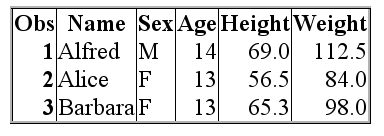
\includegraphics[width=6in]{table_rules.png}
\end{goutput}

\subsection{A Simple Solution}
\index{thead}
\index{Table!thead}
The output looks fine but what is desired is a line between the
Headers and the data.  A little bit of research shows that the
HTML thead tag can have borders.  The thead tag in the output
has no attributes at all.  A border on the bottom
of the tables head section should do the trick.  As confirmation
modifying the thead tag gives the correct look if the
tag looks like this.
\begin{sfvoutput}
<thead style="border-bottom-style: solid;">
\end{sfvoutput}

\subsection{Identify and locate the event}
\index{thead}
\index{Tagsets!HTML4}
\index{Tagsets!HTMLCSS}
\index{Tagsets!PHTML}
\index{Events!table\_head}
Identifying the proper event is easy in this case.
A search for 'thead' in the html tagsets gives us the table\_head event.

It is important to preserve any behavior of the event that is being
redefined.  But in this case there isn't much there.  And the event
is only defined once in the entire htmltags.tpl file.
Looking at the html4 tagset shows no table\_head event.
The parent of html4 is htmlcss, but htmlcss doesn't have a table\_head
event either.  Finally, looking at phtml reveals the table\_head event.
The event is very simple.

\begin{sfvcode}
        define event table_head;
            start:
                put '<thead>' nl;
            finish:
                put '</thead>' nl;
        end;
\end{sfvcode}

\subsection{A Simple Solution}
Changing that will be very simple. The new tagset is shown 
in figure \vref{table_rules1}.
The desired output is shown 
in figure \vref{table_rules1_out}.

\begin{fvcode}{table_rules1}{Columnwise table rules}

proc template;

    define tagset tagsets.table_rules;
        parent=tagsets.html4;

        define event table_head;
            start:
                put '<thead style="border-bottom-style: solid;">' nl;
            finish:
                put '</thead>' nl;
        end;
    end;
run;

ods tagsets.table_rules file='table.html' style=table_rules;
options obs=3;
proc print data=sashelp.class; run;
ods _all_ close;
\end{fvcode}

\begin{goutput}{table_rules1_out}{Columnwise table rules}
\includegraphics[width=6in]{table_rules1.png}
\end{goutput}

\subsection{Table Rules with style}
\index{Events!table\_head}
\index{Styles!table\_head}
Hard coding the style information in the tagset event is certainly
an easy solution.  But there is a better solution.  By using styles
the tagset can be made that will adapt to any need.  All that is really
needed is a style for the table\_head.  Then the tagset needs to use
that style.

Create a new style element for the table\_head is easy.  Setting 
the style on the table\_head
event is also easy.  The only thing that may not be so obvious is that
it is no longer necessary to put a style attribute on the thead tag.
All that is needed is a class attribute that will reference the new
style element.

\subsection{The Better Solution}
The new style and tagset is shown
in figure \ref{table_rules2} on page \pageref{table_rules2}.
The output from this job looks identical to the previous output. The
only difference is the implementation.

\begin{fvcode}{table_rules2}{Table rules with style}

proc template;

    define style styles.table_rules;

        style table /
          borderwidth=3
          bordercolor=black
          rules=cols
        ;

        style table_head /
          borderbottomstyle=solid
        ;
     end;

    define tagset tagsets.table_rules;
        parent=tagsets.html4;

        define event table_head;
            style=table_head;
            start:
                put '<thead'
                putq 'htmlclass=' htmlclass;
                put '>' nl;
            finish:
                put '</thead>' nl;
        end;
    end;
run;

ods tagsets.table_rules file='table.html' style=table_rules;
options obs=3;
proc print data=sashelp.class; run;
ods _all_ close;
\end{fvcode}

This is now a very flexible tagset that will work for anyone.
If no table\_head style is defined then it will behave as always.
But if it is defined, the table head will do whatever is asked 
of it.  

Excercise: Expand on this idea by applying it to the table\_body
and table\_foot events.  Play with the style attributes to see what happens.

\section{Everyone likes stripes}
\index{Table!Striped}
\index{Styles!data}
\index{Styles!dataStrong}
\index{Styles!dataEmphasis}
Another common request is to create tables with striped rows.  This is another
thing that is quite easy to do with styles.  A new style is needed to contrast the
data style already in use.  Then each row should switch between the data style and
the new style.  This is especially easy in SAS 9.1 because of do blocks.

It should be noted, that this can also be done with table templates.  However, 
table templates do not apply to the Report, Tabulate or Print procedures.

\subsection{Defining the Problem}
The goal for this solution is to stripe the data but not the headers or footers.
Reusing existing style elements would be ideal. But creating a new style is not 
out of the question.

\index{Styles!dataStrong}
\index{Styles!dataEmphasis}
\index{Variables!Section}
This is all easy enough to do.  There is a tagset variable called section that
indicates which part of the table the current row is in.  The possible values are head, body,
and foot.  There are also other data style elements available.  Most if not all
styles define dataStrong and dataEmphasis style elements in addition to the data
style.  One of those could be alternated with the data style.  Looking at some of
the style definitions shows that some of them only make the text bold or italic
for these style elements.  That may be too subtle.

For flexibility it would be nice to specify the alternate row style on the ods
statement.  If none is given then the tagset can assume it should use the dataStrong
style.


\subsection{The HTML solution}
\index{Events!classAlign}
\index{HTML!Justification}
\index{HTML!Class}
\index{Tagsets!html4}
\index{Tagsets!htmlcss}
There is no real need to identify and locate these events.  The data, header, row,
and table events figure prominently in most tagsets.
The only real complexity comes when examining the row and data events
in the html4 and htmlcss tagsets.  Instead of just 
printing the htmlclass it triggers an event called classAlign.  This is because
the html output creates a class attribute that has two class names.  One is
for the style and the other is for justification.  Now the classAlign event
needs to be redifined as well. If possible it is best to
preserve the current behavior of any modified events.  In this case the
behavior can be preserved by conditionally limiting the modification to 
only occur when the htmlcass is set to 'data'.

\subsection{The Code}
The finished html tagset is shown below. The striped tabular output is shown 
in figure \ref{striped_table_out} on page \pageref{striped_table_out}.

\begin{fvcode}{striped_table}{The striped table tagset}

proc template;

    define style styles.stripes;
        parent=styles.default;
    
        style DataStripe from data /
            background=cxE0E0E0
        ;
        
    end;
    
    define tagset tagsets.stripes;
        parent=tagsets.html4;

        define event initialize;

            do /if $options;
                 
                set $alt_row_style $options['ROW_STYLE'];
            done;

            set $alt_row_style 'datastrong' /if !$alt_row_style;
        end;

        define event options_set;
            trigger initialize;
        end;

        define event table_head;
            style=table_head;
            start:
                put '<thead';
                putq 'htmlclass=' htmlclass;
                put '>' nl;
                set $row_class 'data';
            finish:
                put '</thead>' nl;
        end;

        define event row;
            start:
                put '<tr>' nl;

            finish:
                put '</tr>' nl;

                do /if cmp(section, 'body');
                    do /if cmp($row_class, 'data');
                        set $row_class $alt_row_style;
                    else;
                        set $row_class 'data';
                    done;
                done;
        end;

        define event classalign;
            do /if cmp(htmlclass, 'data');
                set $class $row_class;
            else;
                set $class htmlclass;
            done;

            unset $vjust;
            unset $just;
            set $vjust vjust / when !cmp("t", vjust);
            set $just just / when !cmp("l", just);
            set $just "r" /when cmp("d", $just);
            break / when !any($class, $just, $vjust);
            put ' class="';
            put $just ' ' $vjust;
            put ' ' $class;
            put '"';
        end;
    end;
run;

ods tagsets.stripes file='striped.html' 
                   options(row_style='datastripe') 
                   style=stripes;
options obs=5;
proc print data=sashelp.class; run;
ods _all_ close;
\end{fvcode}

\begin{goutput}{striped_table_out}{Striped Tables}
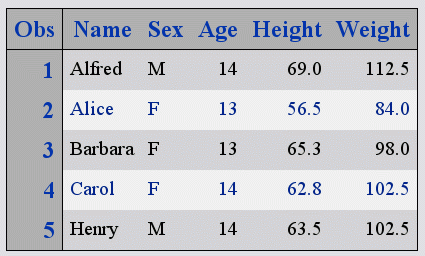
\includegraphics[width=6in]{striped.png}
\end{goutput}

\subsection{The LaTeX solution}
\index{Table!Striped}
\index{LaTeX}
\index{Events!Header}
Doing this same example in LaTeX is even easier.  Mostly because
the LaTeX tagset is not as complicated as the html tagset.
The only difficulty comes from the header event.  The header event
in latex looks like this.
\begin{sfvcode}
        define event header;
            start:
               trigger data;
            finish:
               trigger data;
        end;
\end{sfvcode}

\index{Else}
\index{Statements!Else}
This is fine until the stylename that get's printed is the row\_class
variable.  The result is that all of the header cells are
missing their header references.  The fix was to do this in the data
event.   A Do / else block would be more efficient, but this works
just fine too.
\begin{sfvcode}
        put $row_class /if !cmp(event_name, 'header');
        put htmlclass  /if cmp(event_name, 'header');
\end{sfvcode}

\subsection{The Code}
The finish tagset is shown below. The output is shown 
in figure \vref{striped_table2_out}.

\begin{fvcode}{striped_table2}{Striped tables complete}

proc template;

    define tagset tagsets.striped_latex;
        parent=tagsets.colorlatex;

        define event initialize;

            do /if $options;
                 
                set $alt_row_style $options['ROW_STYLE'];
            done;

            set $alt_row_style 'datastrong' /if !$alt_row_style;
        end;

        define event options_set;
            trigger initialize;
        end;

        define event table_body;
            start:
                set $row_class 'Data';
            finish:
                unset $row_class;
        end;

        define event row;
            finish:
                put CR '\\\hline' CR;

                do /if cmp(section, 'body');
                    do /if cmp($row_class, 'Data');
                        set $row_class $alt_row_style;
                    else;
                        set $row_class 'Data';
                    done;
                done;
        end;

        define event data;
            start:
                put VALUE /if cmp($sascaption, 'true');
                break /if cmp($sascaption, 'true');
                put ' & ' CR / if !cmp(COLSTART, '1') ;

                /* Print cell formatting including class name and alignment. */
                put '   ';
                put '\multicolumn{';
                put colspan;
                put '1' / if !exists(colspan);
                put '}';
                put '{|S{';
                put $row_class /if !cmp(event_name, 'header');
                put htmlclass  /if cmp(event_name, 'header');
                put '}{';
                put just;
                put '}|}';
                put '{';
                put VALUE;

            finish:
                break /if cmp($sascaption, 'true');
                put '}';
        end;
 
    end;
run;

ods tagsets.striped_latex 
    file='striped.tex' 
    style=stripes 
    options(row_style="DataStripe");

options obs=5;
proc print data=sashelp.class; run;
ods _all_ close;
\end{fvcode}


\begin{table}\caption{Striped LaTeX Table}
\label{striped_table2_out}
\begin{sastable}[c]{rllrrr}\hline
   \multicolumn{1}{|S{Header}{c}|}{Obs} & 
   \multicolumn{1}{|S{Header}{c}|}{Name} & 
   \multicolumn{1}{|S{Header}{c}|}{Sex} & 
   \multicolumn{1}{|S{Header}{c}|}{Age} & 
   \multicolumn{1}{|S{Header}{c}|}{Height} & 
   \multicolumn{1}{|S{Header}{c}|}{Weight}
\\\hline
   \multicolumn{1}{|S{RowHeader}{r}|}{ 1} & 
   \multicolumn{1}{|S{Data}{l}|}{Alfred} & 
   \multicolumn{1}{|S{Data}{l}|}{M} & 
   \multicolumn{1}{|S{Data}{r}|}{14} & 
   \multicolumn{1}{|S{Data}{r}|}{69.0} & 
   \multicolumn{1}{|S{Data}{r}|}{112.5}
\\\hline
   \multicolumn{1}{|S{RowHeader}{r}|}{ 2} & 
   \multicolumn{1}{|S{DataStripe}{l}|}{Alice} & 
   \multicolumn{1}{|S{DataStripe}{l}|}{F} & 
   \multicolumn{1}{|S{DataStripe}{r}|}{13} & 
   \multicolumn{1}{|S{DataStripe}{r}|}{56.5} & 
   \multicolumn{1}{|S{DataStripe}{r}|}{ 84.0}
\\\hline
   \multicolumn{1}{|S{RowHeader}{r}|}{ 3} & 
   \multicolumn{1}{|S{Data}{l}|}{Barbara} & 
   \multicolumn{1}{|S{Data}{l}|}{F} & 
   \multicolumn{1}{|S{Data}{r}|}{13} & 
   \multicolumn{1}{|S{Data}{r}|}{65.3} & 
   \multicolumn{1}{|S{Data}{r}|}{ 98.0}
\\\hline
   \multicolumn{1}{|S{RowHeader}{r}|}{ 4} & 
   \multicolumn{1}{|S{DataStripe}{l}|}{Carol} & 
   \multicolumn{1}{|S{DataStripe}{l}|}{F} & 
   \multicolumn{1}{|S{DataStripe}{r}|}{14} & 
   \multicolumn{1}{|S{DataStripe}{r}|}{62.8} & 
   \multicolumn{1}{|S{DataStripe}{r}|}{102.5}
\\\hline
   \multicolumn{1}{|S{RowHeader}{r}|}{ 5} & 
   \multicolumn{1}{|S{Data}{l}|}{Henry} & 
   \multicolumn{1}{|S{Data}{l}|}{M} & 
   \multicolumn{1}{|S{Data}{r}|}{14} & 
   \multicolumn{1}{|S{Data}{r}|}{63.5} & 
   \multicolumn{1}{|S{Data}{r}|}{102.5}
\\\hline
\end{sastable}
\end{table}

\subsection{Summary}
With just a little extra effort the striped tagsets provide enough
flexibility to be useful with any style.  They can even provide
different looks by using different style elements within the chosen
style.  If the style doesn't provide a suitable style element then
it is still easy to inherit from that style and add a single element
to do the striping.

Excercise:  It would be a worthwhile to play with different
styles and style elements to see what sort of striping you might
get.

\section{slidebar columns}
This is a great example of what can be done with a little
imagination.  This example takes advantage of cell widths
as percentages, to create a bar chart affect within a table column.

\subsection{Define the Problem}
The desire is to use a numeric or percentage value and 
create a sliding bar that reflects the value.  If it's a percentage
everything is very easy.  If it is a numeric value then things get
a little more complicated.  Those cases will need some sort of maximum
value to create a percentage from.  Another need is how to
identify the column to use.  For this, styles will be used in a new way.

The HTML implementation of the slidebar is done by creating a table 
inside the data cell.  The table will have 2 cells inside of it.  
The first one will use a percentage width to create a bar.  A little bit of
HTML editing shows that a table cell like this one will give the
desired effect.

\begin{sfvcode}
    <td width="150">
      <table width="100%">
        <td width="72%">72</td><td>&nbsp;</td>
      </table>
    </td>
\end{sfvcode}

\index{Style!Attributes!TagAttr}
\index{Style!Attributes!HTMLClass}
\label{slider}
There is a style attribute called TagAttr.  It stands for Tag Attribute.
TagAttr was meant as a catch all
for any new browser features that styles did not directly accomodate.
Normally anything in TagAttr is printed as is within the tag it belongs
to.  This tagset is going to misuse TagAttr so that proc print can say which columns
should get a slide bar.  It can also be used to give the maximum value for
columns that are not percentages.

\subsection{Identify and Locate}
This step get's easier as tagset events become familiar.  
In this case everything revolves around the data event. 

\subsection{The Solution}
Let's get on with the code. 

\begin{fvcode}{final_slider}{Slider Tagset Complete}
proc template;
    define style styles.slider;
        parent=styles.default;

        style table from output /
            rules=cols
            cellpadding=3
            cellspacing=1
        ;
        style slider from data /
            background=colors('headerbg')
        ;
    end;
  
    define tagset tagsets.slider;
        parent=tagsets.html4;

        define event calculate_width;
            set $width value /breakif index(value, '%') > 0;

            eval $dash_pos index(Tagattr, '-');
            do /if $dash_pos;
                eval $dash_pos $dash_pos+1;
            done;
            eval $value inputn(value, '12.');
            eval $max inputn(substr(Tagattr, $dash_pos), '12.');
            eval $width ($value / $max) * 100;
            set $width $width '%';
            unset $dash_pos;
        end;

        define event data;
            start:
                /* this would work but sometimes htmlclass is empty... */
                trigger header /breakif cmp(htmlclass, "RowHeader");
                trigger header /breakif cmp(htmlclass, "Header");

                do /if index(tagattr, 'slider') > 0;
                    put '<td width="150" class="data">' nl;
                    put '<table width="100%" class="data" cellpadding=0; cellspacing=0;>' nl;
                    trigger calculate_width;
                done;
                put "<td";
                putq ' width=' $width;
                putq " title=" flyover;
                do /if !cmp(htmlclass,'batch');
                    trigger classalign;
                    trigger style_inline;
                done;
                trigger rowcol;
                put " nowrap" /if no_wrap;
                put ">";
                trigger cell_value;

            finish:
                trigger header /breakif cmp(htmlclass, "RowHeader");
                trigger header /breakif cmp(htmlclass, "Header");
   
                trigger cell_value;
                put "</td>" CR;
                do /if $width;
                    put '<td>&nbsp;</td>' CR;
                    put "</table></td>" CR;
                    unset $width;
                done;

        end;
    end;
run;

options obs=3;
ods tagsets.slider file='test.html' style=slider;

proc print data=sashelp.class;
    var name;
    var sex;
    var age;     
    var height / style(data) = slider[just=center tagattr="slider-80"];
    var weight / style(data) = slider[just=center tagattr="slider-150"];
run;

ods tagsets.slider close;
\end{fvcode}        

The output from this example can be seen in figure \vref{slider_out}.
The heart of this example is the data event.  
All it needed was an if block that would create a table with two
cells inside what would ordinarily be a simple data cell.  The first cell
in the slider table is created with the code that normally creates the data
cell.  It just adds the \$width variable if it is there.  The finish
of the data event adds the extra empty cell and closes everything up.

The most complicated part of the tagset is the calculate\_width event.
This is mostly because sliders will work for numeric values as well as
percentages.
If the tagset only worked with pecentages this event wouldn't have been needed.

There is also a short style to make the table look a little nicer.  
Using less cellspacing and padding along with column rules looks nice.  
This example could be combined with the first example in this chapter
for an even nicer look.

The last piece of the puzzle is using the print Procedure's style over-ride
capabilities to turn the sliders on and give a max value to calculate
the percentages from.  A macro variable could have been used to
indicate which columns to use, but this is a little bit nicer.

Excercise:  Create a slider tagset that uses a macro variable or style
over-ride to create sliders on the the columns indicated.

\begin{goutput}{Slider_out}{Slider Columns}
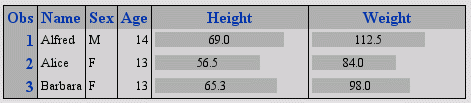
\includegraphics[width=6in]{slider.png}
\end{goutput}

\subsection{Example Summary}
In this example the tagattr style attribute was used to indicate the 
slider columns and the
maximum value.  But since a slider style element was also created the
tagset could just as easily key off of the value of htmlclass and only 
use tagattr to indicate a maximum value if needed.

Exercise: Find and eliminate the extra printing of Tagattr in the data tags.

Exercise: Change the tagset to key off of the style element name instead of
the keyword 'slider' in tagattr.

Exercise: Change the inheritance of this tagset to take advantage of the
changes made to the table\_rules tagset in figure \ref{table_rules2} on page
\pageref{table_rules2}. Combine the table\_rules style with
the slider style.

Exercise: Combine all the examples in the chapter into one tagset.

\section{Summary}
This chapter has shown how styles can be used with tagsets to easily create
nice output.  Using styles can simplify solutions and make those solutions
more adaptable. 

%%\cleardoublepage
%%\chapter{Tagsets with Streams}
\index{Streams}
Streams add another level of versatility to tagsets.  
Streams allow for output to be saved away, and reused or
just delayed.  This is ideal for solving problems where
the ODS event model does not match the shape of the target
ouput. Streams are the most common solution to this problem.
Streams can delay output, collect output from different events
at different times, to be used later.
This chapter will show how to use streams to solve problems
that would otherwise be impossible.

\section{A Tagset with Startpage}
\index{Tagsets!StartPage}
\index{StartPage}
\index{Titles}
\index{Footnotes}
\index{Page breaks}
Several of the ODS destinations have an option called startpage.
Startpage has at least two options, on and off.  On is normal behavior.
Off means that pagebreaks, titles and footnotes are suppressed.  There
are several other possible values for startpage,  the only one that 
makes much sense for a tagset is 'now'.  Now means that the footnotes,
pagebreak and titles should happen next.

ODS markup does not have a startpage option yet.  But startpage behavior
can be implemented with a tagset.  This tagset will use streams to catch the
titles and footnotes.  The emphasis of this tagset is on entirely new
events that have been mostly ignored until now.

\subsection{Identify, Locate and Explore}
Running the code below will give us a nice event map with easy
to find titles and footnotes.

\begin{verbatim}
Title '!!!!!!!!! My New Title !!!!!!!!!';
Footnote '######## My New Footnote ########';
ods tagsets.short_map file='map.xml';
proc print data=sashelp.class; run;
ods tagsets.short_map close;
\end{verbatim}

\index{Events!System\_Title\_setup\_group}
\index{Events!Title\_setup\_container}
\index{Events!System\_Title\_setup}
\index{Events!System\_Footer\_setup\_group}
\index{Events!Footer\_setup\_container}
\index{Events!System\_Footer\_setup}
\index{Events!page\_setup}
What you will find is that the titles and footnotes are listed twice.
Once in a page setup section, and once for each page.  Part of the
resulting output is shown on page \pageref{startpage_out}.
% in \ref{startpage_out} on page \pageref{startpage_out}.

\clearpage
\begin{fvoutput}{startpage_out}{Title and Footnote Events}
      <page_setup>
        <system_title_setup_group>
          <title_setup_container>
            <title_setup_container_specs>
              <title_setup_container_spec/>
            </title_setup_container_specs>
            <title_setup_container_row>
              <system_title_setup value="!!!!!!!!! My New Title !!!!!!!!!">
              </system_title_setup>
            </title_setup_container_row>
          </title_setup_container>
        </system_title_setup_group>
        <system_footer_setup_group>
          <title_setup_container>
            <title_setup_container_specs>
              <title_setup_container_spec/>
            </title_setup_container_specs>
            <title_setup_container_row>
              <system_footer_setup value="######## My New Footnote ########">
              </system_footer_setup>
            </title_setup_container_row>
          </title_setup_container>
        </system_footer_setup_group>
      </page_setup>
      <system_title_group>
        <title_container>
          <title_container_specs>
            <title_container_spec/>
          </title_container_specs>
          <title_container_row>
            <system_title value="!!!!!!!!! My New Title !!!!!!!!!">
            </system_title>
          </title_container_row>
        </title_container>
      </system_title_group>
...
...
...

      <system_footer_group>
        <title_container>
          <title_container_specs>
            <title_container_spec/>
          </title_container_specs>
          <title_container_row>
            <system_footer value="######## My New Footnote ########">
            </system_footer>
          </title_container_row>
        </title_container>
      </system_footer_group>

\end{fvoutput}

\index{Events!System\_Title\_setup\_group}
\index{Events!Title\_setup\_container}
\index{Events!System\_Title\_setup}
\index{Events!System\_Footer\_setup\_group}
\index{Events!Footer\_setup\_container}
\index{Events!System\_Footer\_setup}
The most useful thing about this output is that each set of titles
and footnotes is contained within group events.  There are System\_title\_group
and System\_footer\_group events as well as setup\_group events for each.  the
titles and footnotes can be captured by using those events to advantage.

\subsection{Defining the solution}
Inside the group events, there are title\_container events.  These events
are the same for both the titles and the footnotes.  The behavior of startpage, is
that titles, footnotes and pagebreaks are suppressed.  When it is turned on, titles
and footnotes come out as normal.  But while startpage was off, any footnotes that 
may have occured need to be saved and printed when the output ends, or startpage is
turned back on.   That's where the stream comes in.  It can be used to save the footnotes.

\subsection{Block and Unblock statments}
\index{Statements!Block}
\index{Statements!UnBlock}
\index{Block}
\index{UnBlock}
There are two more statements that will come in handy for this tagset.  The Block and unblock
statements will allow an event to be turned off and on.  One complication is that block and
unblock do reference counting.  In other words, if an event is blocked twice, it will have
to be unblocked twice before it will work again.  This behavior can be defeated by 
compartmentalizing the blocking behavior in an event or two.

\subsection{A partial solution}
\index{Events!pagebreak}
\index{Events!System\_Title}
\index{Events!System\_Footer}
\index{Events!Title\_container\_row}
\index{Events!Title\_container\_spec}
\index{Events!Title\_container\_specs}
A good place to start is to define events to block the titles, footnotes, and pagebreaks.  
By looking at the prevous map it is obvious  the title\_container, title\_container\_row,
system\_footer and system\_title events will need to be blocked.  There may be others
but it depends on what the html tagsets have defined.
This is a good start, if more events need blocking then they can be added later. There 
is no real need to turn anything on or off yet.  This is just a sanity check to see if
this will work as planned.

\index{Events!pagebreak}
\index{Events!Title\_container}
\index{Events!Title\_container\_row}
\index{Statements!Block}
\index{Statements!UnBlock}
\index{Block}
\index{UnBlock}
This example uses a separate event to block the different parts of
the output.  One event to block and unblock the title\_container
events, One each for the system\_title, system\_footer, and pagebreak
events. Each one keeps track of the blocking with a variable.  The
variable either exists with a value of 'True', or it doesn't.  This
keeps the tests simple and effecient. The start section is used to
do the blocking and the finish to do the unblocking. This nicely
compartmentalizes the block and unblock controls.

\begin{fvcode}{startpage1.sas}{Blocking the titles and footnotes}
proc template;
     define tagset tagsets.startpage;
         parent=tagsets.html4;
        /*-------------------------------------------------------eric-*/
        /*-- All titles happen between this event's start           --*/
        /*-- and finish.  redirect them to a stream or              --*/
        /*-- throw them away.                                       --*/
        /*----------------------------------------------------14Aug03-*/
        define event system_title_group;
            start:
                trigger block_title;
                trigger block_title_container;
                trigger block_page_breaks;
            finish:
                trigger block_title;
                trigger block_title_container;
        end;
        
        
        /*-------------------------------------------------------eric-*/
        /*-- All footnotes happen between this event's start        --*/
        /*-- and finish.  redirect them to a stream or              --*/
        /*-- throw them away.                                       --*/
        /*----------------------------------------------------14Aug03-*/
        define event system_footer_group;
            start:
                trigger block_footnote;
                trigger block_title_container;
            finish:
                trigger block_footnote finish;
                trigger block_title_container finish;
        end;
            
        /*--------------------------------------------------eric-*/
        /*-- Block/unblock the titles or footnotes.            --*/
        /*-----------------------------------------------11Aug03-*/
        define event block_title_container;
            start:
                break /if $title_container_blocked;
 
                unblock title_container;
                unblock title_row;
                set $title_container_blocked "true";
             finish:
                unblock title_container;
                unblock title_row;
                unset $title_container_blocked;
        end;
         

        define event block_title;
            start:
                break /if $title_blocked;
 
                block system_title;
                set $title_blocked "true";
            finish:
                unblock system_title;
                unset $title_blocked;
        end;

 
        define event block_footnote;
            start:
                break /if $footnote_blocked;

                block system_footer;
                set $footnote_blocked "true";
             finish:
                 unblock system_footer;
                 unset $footnote_blocked;
        end;
         

        /*-------------------------------------------------------eric-*/
        /*-- block the page breaks                                  --*/
        /*----------------------------------------------------1Aug 03-*/
        define event block_page_breaks;
            start:
                /*-----------------------------------------------eric-*/
                /*-- Only block it once.  Keep the reference count  --*/
                /*-- to one.                                        --*/
                /*--------------------------------------------14Aug03-*/
                do / if ^exists($page_blocked);
                    set $page_blocked "true";
                    block pagebreak;
                done;                   
            finish:
                unblock pagebreak;
                unset $page_blocked;
        end;
    end;
run;

Title '!!!!!!!!! My New Title !!!!!!!!!';
Footnote '######## My New Footnote ########';
ods tagsets.startpage file='startpage.html';
ods html file='startpage_compare.html';
proc print data=sashelp.class;run;
proc print data=sashelp.class;run;
ods _all_ close;

\end{fvcode}

\subsection{The Solution}
\index{Footnotes}
\index{Titles}
\index{page breaks}
Comparing the output from the startpage tagset with the html4 tagset shows that
the titles, footnotes and pagebreaks have been successfully removed.
The next step is to get the titles and footnotes back.  It's time to add a startpage option
to control when that will happen.

If startpage is set to 'no', titles should print once and then stop.  The first footnotes
encountered also need to be saved.  After some footnotes have been captured any footnotes
that follow can be thrown away.

If startpage is set to 'yes' everything is printed as normal.  For convenience, it is 
useful to create a put\_footnotes event that puts the footnote stream and deletes it.

\index{Footnotes}
Since only the first footnotes should print, the footnotes stream should only be opened if
if the stream is empty.  If the stream is not opened, it doesn't hurt anything to 
do a close.  It also doesn't hurt to unblock an event that is already unblocked.  Logic could
be added to avoid doing these unecessary things but the tagset becomes more complex without
any real benefit.
The output can be seen in figure \vref{startpage2_out}.


\begin{fvcode}{startpage2}{Startpage Tagset}
proc template;
    define tagset tagsets.startpage;
        parent=tagsets.html4;
        
        define event initialize;
            unset $start_page_no; 
            do /if $options;
                set $start_page_no "true" /if cmp($options['STARTPAGE']), 'no');
            done;
        end;    

        define event options_set;
            trigger initialize;
        end;

        /*-------------------------------------------------------eric-*/
        /*-- All titles happen between this event's start           --*/
        /*-- and finish.  redirect them to a stream or              --*/
        /*-- throw them away.                                       --*/
        /*----------------------------------------------------14Aug03-*/
        define event system_title_group;
            start:
                do /if $start_page_no;
                    do /if $titles_printed;
                        trigger block_title;
                        trigger block_title_container;
                    done;
                    set $titles_printed "true";

                    /*------------------------------------------eric-*/
                    /*-- Block the page breaks after the first     --*/
                    /*-- titles have been printed.  Otherwise we   --*/
                    /*-- don't get a pagebreak when we switch from --*/
                    /*-- start_page=yes to start_page=no.          --*/
                    /*---------------------------------------11Aug03-*/
                    trigger block_page_breaks start;
                done;
            finish:
                trigger block_title;
                trigger block_title_container;
        end;
        
        
        /*-------------------------------------------------------eric-*/
        /*-- All footnotes happen between this event's start        --*/
        /*-- and finish.  redirect them to a stream or              --*/
        /*-- throw them away.                                       --*/
        /*----------------------------------------------------14Aug03-*/
        define event system_footer_group;
            start:
                do /if exists($$footnotes);
                    trigger block_footnote;
                    trigger block_title_container;
                else;
                    open footnotes;
                done;

            finish:
                close;
                unset $footnotes_open;
                trigger block_footnote;
                trigger block_title_container;

                trigger put_footnotes /if ^$start_page_no;
        end;
            

        /*-------------------------------------------------------eric-*/
        /*-- Write out the footnotes we saved earlier.              --*/
        /*----------------------------------------------------14Aug03-*/
        define event put_footnotes;
            put $$footnotes;
            unset $$footnotes;
        end;
        
            
        /*--------------------------------------------------eric-*/
        /*-- Block/unblock the titles or footnotes.            --*/
        /*-----------------------------------------------11Aug03-*/
        define event block_title_container;
            start:
                break /if $title_container_blocked;
 
                unblock title_container;
                unblock title_row;
                set $title_container_blocked "true";
             finish:
                unblock title_container;
                unblock title_row;
                unset $title_container_blocked;
        end;
         

        define event block_title;
            start:
                break /if $title_blocked;
 
                block system_title;
                set $title_blocked "true";
            finish:
                unblock system_title;
                unset $title_blocked;
        end;

 
        define event block_footnote;
            start:
                break /if $footnote_blocked;

                block system_footer;
                set $footnote_blocked "true";
             finish:
                 unblock system_footer;
                 unset $footnote_blocked;
        end;
         

        /*-------------------------------------------------------eric-*/
        /*-- block the page breaks so we don't get them inside the panel.--*/
        /*----------------------------------------------------1Aug 03-*/
        define event block_page_breaks;
            start:
                /*-----------------------------------------------eric-*/
                /*-- Only block it once.  Keep the reference count  --*/
                /*-- to one.                                        --*/
                /*--------------------------------------------14Aug03-*/
                do / if ^exists($page_blocked);
                    set $page_blocked "true";
                    block line;
                    block pagebreak;
                done;                   
            finish:
                unblock line;
                unblock pagebreak;
                unset $page_blocked;
        end;

    end;
run;

Title '!!!!!!!!! My New Title !!!!!!!!!';
Footnote '######## My New Footnote ########';

options obs=1;

ods tagsets.startpage file='startpage.html' options(startpage='no');
proc print data=sashelp.class;run;
proc print data=sashelp.class;run;
ods _all_ close;

\end{fvcode}

\begin{goutput}{startpage1_out}{Start Page Working}
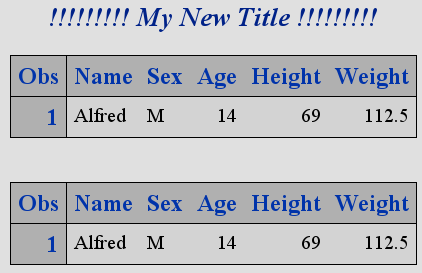
\includegraphics[width=6in]{startpage1.png}
\end{goutput}


\subsection{More Identify and Locate}
\index{Footnotes}
\index{Events!doc\_body}
So far so good, but where are the footnotes? They never get printed
because startpage is always no! Something needs to print them when
the document finishes, regardless of the setting of startpage.
Looking at the HTML from the first example it can be seen that the
footnotes came out right above the closing </body> tag.  Looking
through the html tagsets for the body tag gives away the the doc\_body
event.  The html4 tagset inherits the doc\_body event from the htmlcss
tagset.  All that is needed is to trigger the put\_footnotes event
in the finish of the doc\_body event.  There won't be any footnotes
to print if they've been printed already.

\begin{sfvcode}
proc template;
    define tagset tagsets.startpage2;
        parent=tagsets.startpage;
        
        define event doc_body;
            start:
                put '<body onload="startup()"';
                put ' onunload="shutdown()"';
                put  ' bgproperties="fixed"' / WATERMARK;
                putq " class=" HTMLCLASS;
                putq " background=" BACKGROUNDIMAGE;
                trigger style_inline;
                put ">" CR;
                trigger pre_post;
                put          CR;
                trigger ie_check;

            finish:
                trigger put_footnotes;

                trigger pre_post;
                put "</body>" CR;
        end;
    end;
run;

Title '!!!!!!!!! My New Title !!!!!!!!!';
Footnote '######## My New Footnote ########';

options obs=1;

ods tagsets.startpage2 file='startpage.html' options(startpage='no');
proc print data=sashelp.class;run;
proc print data=sashelp.class;run;
ods _all_ close;
\end{sfvcode}

\begin{goutput}{startpage2_out}{Start Page Working}
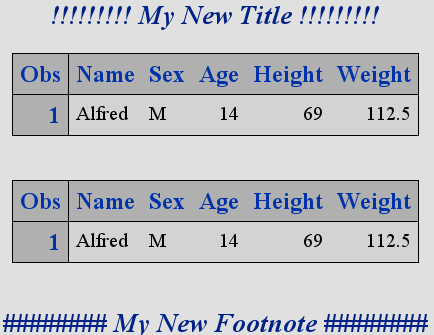
\includegraphics[width=6in]{startpage2.png}
\end{goutput}


\begin{sfvcode}
proc template;
/* start it off with startpage=no. */
ods tagsets.startpage2 options(startpage="no") file="startpage.html";

proc print data=sashelp.class; run;

proc print data=sashelp.class; run;

ods tagsets.startpage2 options(startpage="yes");

proc print data=sashelp.class; run;

proc print data=sashelp.class; run;

ods tagsets.startpage2 options(startpage="no");

proc print data=sashelp.class; run;

proc print data=sashelp.class; run;

ods _all_ close;
\end{sfvcode}

\begin{goutput}{startpage3_out}{Start Page }
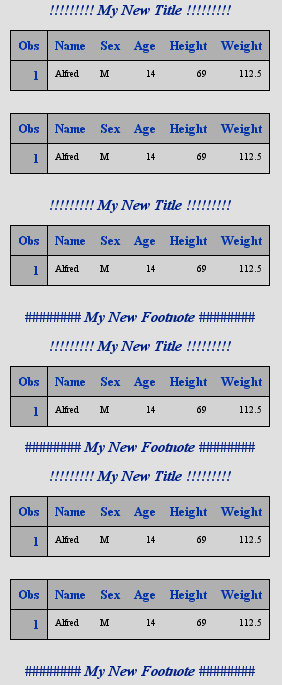
\includegraphics[width=3in]{startpage3.png}
\end{goutput}

\subsection{The Final Solution}
The output is shown in figure \vref{startpage3_out}.

\subsubsection{More exploration}
But there is something wrong.  The footnotes are missing from the first section. 
All the pagebreaks are missing.  Sprinkling a few putvars and putlog statements
through this tagset is helpful.

The startpage event is a boundry condition.  The footnotes need to be printed when
the value of start\_page changes to yes.  The pagebreaks are missing because they
get blocked once after the first titles are printed.  The startpage event needs
to unblock them in order for everything to return to normal.

Changing the startpage event to the following will fix everything.
The output is shown in figure \vref{startpage4_out}.

\begin{sfvcode}
        define event startpage;
            /*---------------------------------------------------eric-*/
            /*-- if we got a value check set start page,            --*/
            /*-- if we didn't get a value then set it               --*/
            /*-- to the alias we got on the initial ods             --*/
            /*-- statement.                                         --*/
            /*------------------------------------------------11Aug03-*/
            unset $start_page_no;

            do /if value;
                set $start_page_no 'true' /if cmp(value, 'no');
            else;
                set $start_page_no 'true' /if cmp(tagset_alias, 'no');
            done;
            
            do /if !$start_page_no;
                unset $start_page_no;
                unset $titles_printed;

                trigger put_footnotes;
                trigger block_page_breaks finish;
            done;
        end;
\end{sfvcode}

\begin{goutput}{startpage4_out}{Start Page - Final Version}
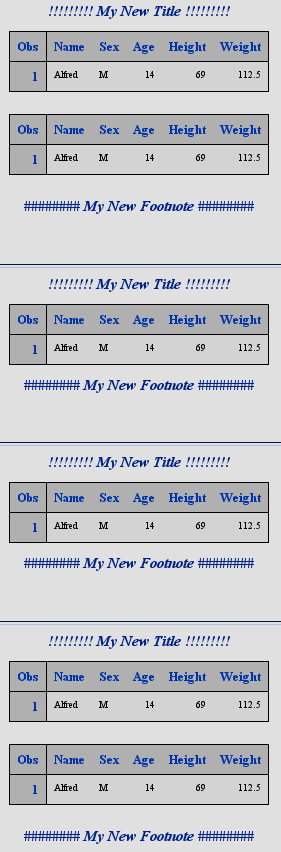
\includegraphics[width=3in]{startpage4.png}
\end{goutput}


\section{Summary}
Streams are one of the most powerful features available in tagsets.
They can be used to delay and repeat output or rearrange output to
fit your needs.  Streams do expose some difficulties presented by 
specific procedures but with careful consideration, thought and 
maybe a little frustration, those problems can be overcome.


%%\cleardoublepage
%%\chapter{ODS Output for Website Integration}
\index{Website Integration}
\index{Website Templates}
Many web sites have a framework that web pages must fit into 
before they will be published.  Usually this means
editing the html pages and pasting in some chunk of HTML from
some files the website authors have provided.
Usually there is one file to replace the top section of the
web page and another to replace the bottom.  
The tagsets in this chapter will create HTML that
is ready for integration with any website.  

\section{The Problem}
Most websites want webpages to be enclosed with some sort of
image and navigation menu at the top and/or bottom.  Most of this
is usually enclosed in some sort of table to control the layout.

This enclosing HTML is usually put in two files so that it is easy
to include them as the top and bottom of each web page.  Prior to
SAS 9.1 there were two ways to do this.  The hardest way is to use
the no\_top and no\_bot options along with some datastep to write
the file templates.  Starting with SAS 8.2 it became possible to
create a tagset that included the text from the website's framework
files.  This is really the simplest way to do this, but it leads
to dual maintenance because everytime the files change, the tagset
needs to have the same changes.

\index{Website Integration}
\index{Website Templates}
\index{Statements!Putl}
\index{Putl}
If that is the route you wish to take there is a put command that
will help.  'Putl' is just like put except that it has an automatic
newline at the end.  That means you can copy and paste in a block
of text and place a putl ' at the beginning and a '; at the end of
each line.  That's not too hard but can be painful if the framework
files change very often.

The framework files usually include everything that goes in an HTML
document down to and including the body tags.  All of your content
goes inbetween with no need to define the basic HTML document.  At
the very least the solution needs to eliminate the output from the
events above the start and below the finish of the doc\_body event.

The most difficult part of this is that somehow, the stylesheet for
the ODS output will have to be incorporated into the middle of the
framework text.  If your web designers are nice, they may be willing
to place an ods generated stylesheet with their other stylesheets.
They may even put a reference to it in their framework file.  In
that case the tagset will be easy.  Either way, a working tagset
can be created.

\section{Alternate Behavior for existing options}
The first step towards this solution is to eliminate all the events
above and below the body tags.  ODS already gives options to do
that.  All that is needed is to detect when those options are set.
Then detect if there are files that can be used in place of the
head and foot sections of the document.

\index{Options!No\_Top\_Matter}
\index{Options!No\_Bottom\_Matter}
\index{Options!No\_Top}
\index{Options!No\_Bot}
\index{Variables!No\_Top}
\index{Variables!No\_Bot}
Macro variables, or alias can be used to specify the files to read.
If both the no\_top\_matter and no\_bottom\_matter options are used
with file name specifications, then the tagset can behave as desired.
Otherwise normal behavior will be the way to go.

\subsection{Explore}
Running an event map with the notop and nobot options shows that there are variables in
the tagset called no\_top and no\_bot that indicate these options were set.  That will
be very useful.

\index{Events!Initialize}
The trick to this tagset is using the initialize event to advantage.  The initialize
event always happens.  But when no\_top and no\_bot is used the first and last events
are somewhat variable.   The first event could be system\_titles, or not.  The last could
be system\_footers, or not.  Reviewing the available events shows that no\_bot causes
the end to be unpredictable.  Luckily there are not that many events in the bottom
section of an html document.  As usual, the initialize event can be used to set things up, and
redefine the events in the bottom section to do the right thing.  That means that
all the external controls need is the no\_top option with some method of passing two 
filenames to read.

\section{Reading an external file}

\index{Functions!filename}
\index{Functions!fopen}
\index{Functions!fread}
\index{Functions!fget}
\index{Functions!Return Code}
\index{Statements!Eval}
\index{Statements!Set}
\index{DataStep!Functions}
The key to this tagset is reading an external file.  That example is shown
on page \pageref{readfile}.  This example will build on that functionality.

Your website's authors will probably have two files that may resemble the following
HTML code.  The top section defines the html document and starts the body section
of the page and creates some tables for layout.  There is a table along the top for
the Company logo and navigation.  Below that is another table with one row and three
cells.  The first cell contains another table with more navigation menus.  the second
cell is where The sas output will go.  The second file closes everything up, puts a
table across the bottom for more navigation, contacts, copyright notices and the like.

\begin{Verbatim}[frame=lines, framesep=3mm, label={Sample}]

<!DOCTYPE html PUBLIC "-//W3C//DTD XHTML 1.0 Transitional//EN"
    "http://www.w3.org/TR/xhtml1/DTD/xhtml1-transitional.dtd">

<html xmlns="http://www.w3.org/1999/xhtml">
  <head>
    <meta name="generator" content="HTML Tidy, see www.w3.org" />
    <meta content="text/html; charset=iso-8859-1"
    http-equiv="Content-Type" />

    <title>Your website name</title>
    <meta name="description" content="Your website name" />
    <meta name="keywords" content="SAS, ODS, Markup, HTML, XML" />

    <link rel="shortcut icon" href="/favicon.ico" type="image/x-icon" />
    <link rel="icon" href="/fav_icon.ico" type="image/x-icon" />
    <style type="text/css">
    <!--
    .main{Background-color:#E0E0E0;
          color:#000000;
         }

    a:link { color:#0066AA }
    a:visited { color:#004488 }
    a:active { color:#004488 }

    .layout_table{cellspacing: 0;
                  padding: 0;
                  borderwidth: 0px;
                  width: 100%;
         }
    .nav_table{cellspacing: 0;
                  borderwidth: 0px;
                  width: 50px;
                  background-color: #00DD55;
         }
    .nav_label{color: #000088;
               font-size: medium;
               font-weight: bold;
         }
    .output_cell{color: #E0E0E0;
         }
    </style>
  </head>

  <body class="main">

    <!-- Beginning of Top headline and navigation table -->
    <table class="layout_table">
      <tr>
        <td><a href="http://www.yourdomain.org/index.html">
        <img src="gifs/logo.gif" height="94" width="306"
        alt="Logo Image alt text: Your Company: Slogan" border="0" /></a>
        </td>

        <td align="right" valign="bottom">

          <form action="http://www.yourdomain.org/cgi/region.cgi"
          method="get">
            <br />
            <span class="nav_label">Select your Region:</span>
            <br />
            <select name="goto">
              <option value="http://www.yourdomain.org/region1"> Region 1 </option>

              <option value="http://www.yourdomain.org/region2">
                Region 2
              </option>

              <option value="http://www.yourdomain.org/region3">
                Region 3
              </option>

              <option value="http://www.yourdomain.org/region4">
                Region 4
              </option>

              <option value="http://www.yourdomain.org/region5">
                Region 5
              </option>

              <option value="http://www.yourdomain.org/region6">
                Region 6
              </option>
            </select><input type="submit" value=" Go " /><br />

          </form>
        </td>
      </tr>
    </table>
    <hr size="1" noshade="noshade" />

    <!-- Beginning of main table -->
    <table class="layout_table">
      <tr>

        <!-- Beginning of Left Side Navigation Bar. -->
        <td valign="top">
          <table class="layout_table">
            <tr>
              <td>
                <table class="nav_table">
                  <tr>
                    <td>
                      <p><font class="nav_label"><b>News</b></font>
                      <small><br />

                       <a href="news/newsflash.html">Announcements</a><br />

                       <a href="news/press.html">In the Press</a><br />
                       <a href="news/index.html">More ...</a>
                       </small></p>

                      <p><font class="nav_label"><b>Company</b></font>
                      <small><br />

                       <a href="./contact/index.html">Contact Information</a><br />
                       <a href="./about/index.html">About</a><br />
                      </small></p>

                      <form action="http://www.yourdomain.org/cgi/search.cgi"
                       method="get">

                        <small>Search for:<br />
                        <input type="text" name="words" size="10" />
                        <input type="hidden" name="max" value="25" />
                        <input type="hidden" name="source" value="www" />
                        <input type="submit" value="Go" />
                        </small>
                      </form>
                    </td>
                  </tr>
                </table>
              </td>
            </tr>

          </table>
        </td>
        <!-- End of Left Side Navigation Bar. -->

        <!-- Beginning of Center - Output Panel -->
        <td class="output_cell">
\end{Verbatim}

The ending of your website's pages may look something like this

\begin{Verbatim}[frame=lines, framesep=3mm, label={Sample2}]
        </td>
        <!-- End of Center - OutputPanel -->

        <!-- beginning of Right - Navigation Panel -->
        <td align="right">
           <table class="nav_table" >
             <tr><td>
               <ul>
                 <li> More Navigation:</li>
                 <ul>
                   <li> Navigation1</li>
                   <li> Navigation2</li>
                 </ul>
               </ul>
             </td></tr>
           </table>
        </td>
        </tr>
    <!-- End of Middle - Layout table -->
   </table>

   <table class="layout_table" >
   <tr>
   <td align="center">
    <hr size="1" noshade="noshade" /><br/>
       Copyright 2004 Your Company name. 
   </td>
   </tr>
   </table>

</body>
</html>
\end{Verbatim}

\section{The Solution}
The following tagset will read the files given through the tagset alias or 
a macro variable called infiles.  Alias or infiles should be two
filenames separated by a space.   
If tagset alias is set to 'default' then the 
set\_default\_files event is used to set the default file names.
By using a separate event, this tagset can be used as a parent
tagset, where only the set\_default\_files event is redefined.
This also allows normal no\_top behavior if no files are specified.  

Another key to this tagset is that only external stylesheets are
allowed.  It is possible to make embedded stylesheets work.  But
that behavior is not really desirable in this case because our network
administrators wouldn't like embedded stylesheets in our files.  
A stylesheet file must be specified on the ods statement when using
this tagset.

\subsection{Initialization Timing}
\index{Tagsets!short\_map}
\index{Events!Proc}
\index{Events!Initialize}
\index{Events!Initialize!Timing}
\index{Files!Stylesheet}
\index{Variables!No\_Top}
Upon trying this method with the stylesheet option, it can be seen that the initialize event
doesn't work quite right.  That's because initialize happens once.  At the very beginning.
The stylesheet file is created before the body file, so that's when it happens.  No\_top isn't
set for the stylesheet, so the head section of the body file is never printed.  
The solution can be found
by running the same output through the short\_map tagset - with the same ods statement options.
What can be seen is that the proc event always comes out the first thing.  Using the first
proc event to print the top of the file template will work just fine.
 
The best solution is for the website's templates include an ods stylesheet. 
In that case specifying a stylesheet on the ods statement won't be 
necessary.  That would also insure that all ODS output always matches
the website.  All things considered this is still a fairly simple tagset.  The
most complex parts are the things that make it work invisibly for users
who don't want or need this special behavior.

\begin{fvcode}{Web_integration}{Website integration Tagset}
/*----------------------------------------------------------------*/
/*-- Reading a file in using datastep functions.  This example  --*/
/*-- comes straight out of the online documentation             --*/
/*-- for fread().                                               --*/
/*----------------------------------------------------------------*/
proc template;
    define tagset tagsets.website;
        parent=tagsets.html4;
        embedded_stylesheet=no;

        define event initialize;

            do /if $options;
               do /if $options['HEAD_FILE']; 
                   set $head_file $options['HEAD_FILE'];
               done;
               do /if $options['FOOT_FILE']; 
                   set $foot_file $options['HEAD_FILE'];
               done;
               do /if cmp($options['DEFAULT_FILES'], 'yes'); 
                    set $head_file 'default_head.html' /if ^$head_file;
                    set $foot_file 'default_foot.html' /if ^$head_file;
               done;
            done;

            putlog "Infiles are" " :" $head_file "  " $foot_file;

            set $filename $head_file;

            /*--------------------------------------------eric-*/
            /*-- Set a flag so the ending document tags      --*/
            /*-- can be suppressed.                          --*/
            /*-----------------------------------------8Nov 03-*/
            do /if $infiles);
                set $read_files 'true';
                set $filrf "headfile";
                set $read_head "true";
            done;
        end;

        define event proc;
            start:
                do /if no_top;
                    do /if $read_head;
                        trigger readfile;
                        unset $read_head;
                    done;
                done;
        end;


        define event head_search;
            trigger integrated_link /if contains($file_record, '</head>');
        end;

        define event integrated_link;
            put '<style type="text/css">' CR '<!--' CR;
            trigger alignstyle;
            put '-->' CR '</style>' CR ;
        
            set $urlList stylesheet_url;
            set $urlList stylesheet_name /if !$urlList;
            trigger urlLoop ;
            unset $urlList;
        end;

        define event readfile;
            
            /*------------------------------------------------*/
            /*-- Set up the file and open it.               --*/
            /*------------------------------------------------*/
            putlog "Reading in file: " $filename;

            eval $fid 0;
            
            eval $rc filename($filrf, $filename);
            
            eval $fid fopen($filrf);
            do /if missing($fid);
                putlog "Error: Could not open file, " $filename;
                break;
            done;


            /*---------------------------------------------------*/
            /*-- datastep functions  will bind directly to the --*/
            /*-- variable space as it exists.                  --*/
            /*--                                               --*/
            /*-- Tagset variables are not like datastep        --*/
            /*-- variables but we can create a big one full    --*/
            /*-- of spaces and let the functions write to it.  --*/
            /*--                                               --*/
            /*-- This creates a variable that is 200 spaces so --*/
            /*-- that the function can write directly to the   --*/
            /*-- memory location held by the variable.         --*/
            /*-- in VI, 200i<space>                            --*/
            /*---------------------------------------------------*/
            set $file_record  "

                                  ";

            /*-------------------------------------------------*/
            /*-- Loop over the records in the file           --*/
            /*-------------------------------------------------*/
            do /if $fid > 0 ;

                do /while fread($fid) = 0;

                    set $rc fget($fid,$file_record ,200);

                    trigger head_search;
                    
                    /* trimn to get rid of the spaces at the end. */
                    put trimn($file_record ) nl;

                done;
            done;

           /*----------------------------------------------------*/
           /*-- close up the file.  set works fine for this.   --*/
           /*----------------------------------------------------*/

            set $rc close($fid);
            set $rc filename($filrf);

        end;

        define event doc;
            start:
                set $doctype '<!DOCTYPE html PUBLIC "-//W3C//DTD HTML 4.01 Transitional//EN">';
                set $framedoctype '<!DOCTYPE html PUBLIC "-//W3C//DTD HTML 4.01 Frameset//EN">';
                put $doctype CR;
                put "<html>" CR;

            finish:
                do /if $read_files;
                    set $filename scan($infiles, 2, ' ');
                    set $filrf "footfile";
                    trigger readfile;
                    break;
                done;

                put "</html>" CR;
        end;

        define event doc_body;
            put '<body onload="startup()"';
            put ' onunload="shutdown()"';
            put  ' bgproperties="fixed"' / WATERMARK;
            putq " background=" BACKGROUNDIMAGE;
               trigger style_inline;
            put ">" CR;
            trigger pre_post;
            put          CR;
            trigger ie_check;

          finish:
            trigger pre_post;

            break /if $read_files;
            put "</body>" CR;
        end;

end;

run;


ods tagsets.shortmap stylesheet="stylesheet.map" 
                          file="website.map"(notop) ;

ods tagsets.website stylesheet="website.css" 
                          file="website.html"(notop) 
                         options(default_files = 'yes');

proc print data=sashelp.class; run;
    
ods tagsets.website close;
ods _all_ close;
\end{fvcode}

\section{Summary}
\index{Website Integration}
The output using these particular template files is shown 
in figure \vref{website_out}.  
Working with the authors of your website should enable you to create some very
nice looking output.  All of which is immediately ready for integration.
        
\begin{goutput}{startpage2_out}{Website integration}
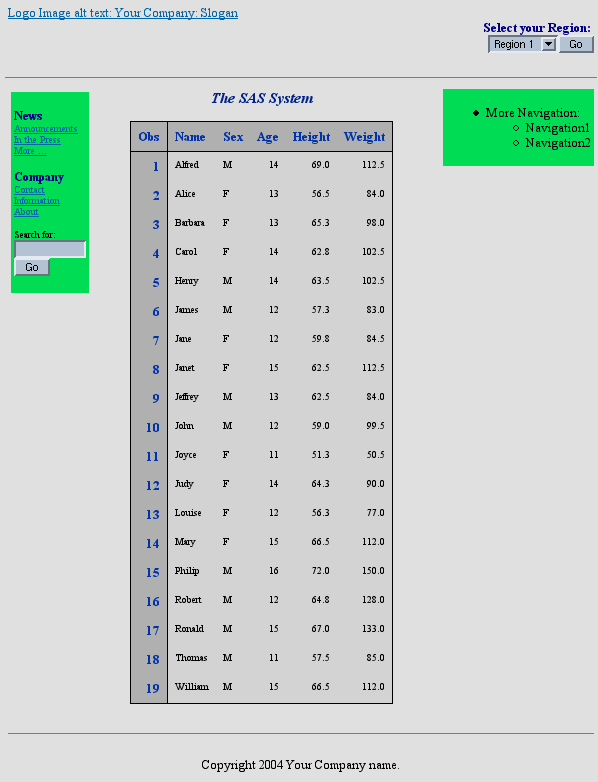
\includegraphics[width=6in]{website.png}
\end{goutput}

%%\cleardoublepage
%%\chapter{Datastep Conversions}
\index{DataStep Conversions}
You may wonder, why would someone want to convert a datastep 
program to use tagsets?  There are lots of reasons.  Mostly it's
for code reuse and flexibility.  Datastep programs allow lots of
flexibility but they are written for one purpose.  If the same 
functionality is desired for a different set of data an entirely
new datastep will have to be written.  If the rendering is left to
a tagset, then anyone can use that tagset with any form of data,
and any procedure.  Maintenance of the code is also simplified 
since both the tagset and the resulting SAS job wil be much
simpler than the original datastep. Add the various powers of
ODS to this new found flexibility and there is plenty of motivation
for conversion.  This chapter will show the process and rewards 
of converting datastep programs to tagsets. 

\index{DDE}
\index{CSV}
\index{XML}
Yet another reason to
convert is that tagsets can be interchanged to create new and 
diffrent outputs.  Usually datastep is used to create HTML, CSV,
or DDE to XML,  A different datastep is required for each.  A different
tagset is required for each as well.  The difference is the reusability
and the ease of creation and maintenance.

\index{ODS}
\index{ODS!Styles}
\index{ODS!Select}
\index{ODS!Exclude}
\index{ODS!Document}
Full integration with ODS provides more than enough reasons to convert 
a datastep to a tagset.  Ods styles, table templates, select and exclude,
and proc document are very good reasons.  There are many other things that
ODS can do besides these, but not if datastep is the method of creating the
output.

\section{Special Bylines}
\index{nobs}
\index{Counting Observations}
\index{Bylines}
One of the things that can be done in datastep is the counting of observations
for display in the byline.  The datastep just counts them first then another
datastep prints everything out.  Tagsets can do that too.  This first example
has a special style, as well as a special byline.  The byline text may change
based upon the current by value.  Each byline also displays the number of
observations in the table below it.  

\subsection{The DataStep Code}
\index{Procedures!Report}
\index{Highlighting}
The original datastep code is shown below.  It has been simplified to use
the sashelp.class dataset.  There is nothing very hard about this code.  The
worst thing is all the puts.  The original data step also did some highlighting
and value translation.  Both of those things are much easier to do using the report procedure.
Another nice thing this datastep does is put the web page title in the title tag and
as the heading on the page.  This is also easy to do with a tagset. The original
output can be seen in figure \vref{ages_out}.

\begin{sfvcode}
filename webout 'ages.html';

%let numfuture=16;

proc sort data=sashelp.class out=myclasssrt;
  by age name weight;
run;

/* Count number of items in each BY group */
data cnt_by_obs;
   keep cnt;

   set work.myclasssrt;
   by age;

   if first.age then curcnt = 0;
   curcnt + 1;
   if last.age then do; cnt = curcnt; output; end;
run;

options missing='-';
data _null_;
   file webout;
   if _N_ = 1 then do;
      length title $ 128;
      length stoday stime $ 8;
      retain linecnt 1;

      stoday = put( today(), date7. );
      stime = put( time(), time5. ); 
      title = 'Class List &nbsp;-&nbsp; ' || stoday || "at " || stime;
      put '<!DOCTYPE HTML PUBLIC "-//IETF//DTD HTML//EN">';
      put '<HTML><HEAD>';
      put '<TITLE>' title '</TITLE>';
      put '</HEAD><BODY>';
      put '<CENTER><H3>' title '</H3></CENTER>';
   end;

   set work.myclasssrt;
   by age;

   if _N_ = 1 or FIRST.age then do;
      length lab $ 32;
      set work.cnt_by_obs;
      if age >= &numfuture then do;
         put '<CENTER><B><FONT SIZE=+2>The Oldest</FONT> ' @;
         put '<FONT SIZE=-1>(' cnt +(-1) ' '@;
         if cnt = 1 then
            put 'entry)' @;
         else
            put 'entries)' @;
         put '</FONT></B></CENTER>';
      end;
      else do;
         put '<CENTER><B><FONT SIZE=+2>Age is ' age '</FONT> ' @;
         put '<FONT SIZE=-1>(' cnt +(-1) ' '@;
         if cnt = 1 then
            put 'entry)' @;
         else
            put 'entries)' @;
         put '</FONT></B></CENTER>';
      end;
      put '<TABLE ALIGN=CENTER VALIGN=MIDDLE>';
      put '<TR>';
      lab = vlabel(Name);         put '<TH>' lab '</TH>';
      lab = vlabel(Weight);       put '<TH>' lab '</TH>';
      lab = vlabel(Height);       put '<TH>' lab '</TH>';
      lab = vlabel(Sex);          put '<TH>' lab '</TH>';
      put '</TR>';
   end;

   if mod(linecnt,2) then
      put '<TR ALIGN=CENTER VALIGN=MIDDLE BGCOLOR="D5E5D2">';
   else
      put '<TR ALIGN=CENTER VALIGN=MIDDLE>';

   put '<TD ALIGN=CENTER>' name '</TD>';
   put '<TD><FONT SIZE=-1>' weight '</FONT></TD>';
   put '<TD><FONT SIZE=-1>' height '</FONT></TD>';
   put '<TD><FONT SIZE=-1>' sex '</FONT></TD>';
   put '</TR>';

   linecnt + 1;

   if LAST.age then do;
      put '</TABLE>';
      linecnt = 1;
      put '<BR><HR><BR>';
      put '</BODY></HTML>';
   end;
run;

\end{sfvcode}

\begin{goutput}{ages_out}{Data step}
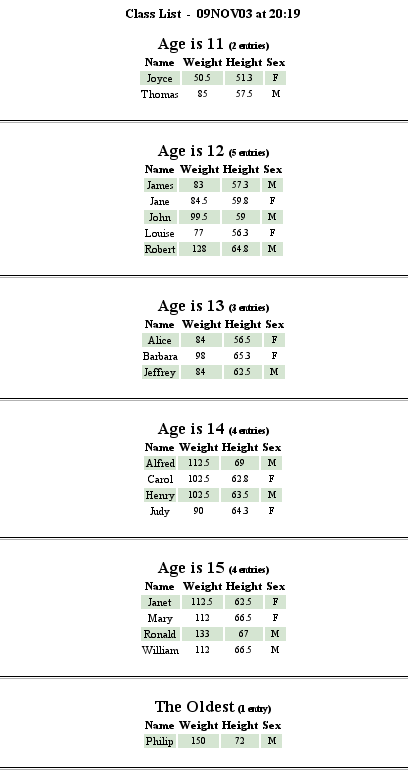
\includegraphics[width=4in]{ages.png}
\end{goutput}


\subsection{Breaking it down}
\index{Styles!Minimal}
The best way to approach a problem like this is to break it down into separate
problems.  In this case there is a fairly minimalist set of colors and fonts.
A fairly simple ODS style can be created from what can be seen in the datastep code.

\index{Tables!striping}
The next problem is striping of tables.  That problem was solved in the example on
page \pageref{striped_table}.
So this new tagset can use the stripes tagset as it's parent.  

\index{Byline!Modifying}
\index{Counting Observations}
There are three more things to solve, Extending the use of the title, counting the 
observations, and modifying the byline.  It would be perfectly
reasonable to solve both those problems in one tagset.  But the last
tagset is simpler if an
intermediate tagset is created to count the observations and display the count.
As a bonus the intermediate tagset can be used in other jobs to solve
other problems because it is not specific to this specific problem.

\subsection{The Style}
\index{Styles!Minimal}
Extracting all the colors and fonts from the datastep is easy enough.  
With something this simple the best thing is to use the minimal style as
a parent.  The minimal style will provide everything that is needed 
without making things complicated.
The resulting style looks like this.

\begin{sfvcode}
    define Style styles.minimal_striped; 
        parent = styles.minimal;

        style header/
            font = (, 4,bold)
        ;

        style Data/
            font = (, 3,normal)
        ;

        style DataStrong from data /
            background=cxD5E5D2
        ;

        replace Output /
            BorderWidth = 0
            CellSpacing = 1
            CellPadding = 7
            Frame = void
            Rules = none
        ;

    end;
\end{sfvcode}


\subsection{Counting Observations}
\index{Observation Count}
\index{Number of Observations}
\index{nobs}
\index{Variables!Macro}
The new tagset inherits from tagsets.stripes from page \pageref{striped}. 
This tagset manipulates the title and prints it as a heading. 
We also add a counter for the observations, and a stream to catch
the table while the observations are being counted.  The last thing is to add
an event to print the observation count.
A macro variable called do\_nobs\_label must be set to 'true' for the observation
counting to take effect.  Otherwise the tagset will exhibit normal behavior.
This tagset will work for any tabular output that ods creates.  
The new tagset looks like this.  
The Output is shown in listing \vref{ages2_out}.

\begin{sfvcode}
proc template;
    define tagset tagsets.nobs_label;
        parent=tagsets.stripes;

        define event initialize;
            unset $do_nobs;
            do /if $options;

                set $do_nobs "true" /if cmp($options['NOBS_LABEL']), 'yes');

                /*---------------------------------------------------eric-*/
                /*-- From the stripes tagset.                           --*/
                /*------------------------------------------------9Nov 03-*/
                set $alt_row_style $options['ALTERNATE_STYLE']";
            done;

            set $alt_row_style 'DataStrong' /if !$alt_row_style;
        end;    

        define event options_set;
            trigger initialize;
        end;

        /*-------------------------------------------------------eric-*/
        /*-- Add the date and time to the document title.  Save it  --*/
        /*-- away for later.                                        --*/
        /*----------------------------------------------------7Aug 03-*/
        define event doc_title;
              break /if ^value;
              set $title value '&nbsp;-&nbsp;' date " at " time; 
              putl '<TITLE>' $title '</TITLE>';
        end;

        define event doc_body;
            start:
                put '<body onload="startup()"';
                put ' onunload="shutdown()"';
                put  ' bgproperties="fixed"' / WATERMARK;
                putq " class=" HTMLCLASS;
                putq " background=" BACKGROUNDIMAGE;
                trigger style_inline;
                put ">" nl;
                trigger pre_post;
                put          nl;
                trigger ie_check;

                /*-----------------------------------------------eric-*/
                /*-- This is the part that changed.                 --*/
                /*-- Add in the title if we have one.               --*/
                /*--------------------------------------------7Aug 03-*/
                do /if $title;
                    putl '<h3';
                    trigger align;
                    putl '>' $title '</h3>';
                done;

            finish:
                trigger pre_post;
                put "</body>" nl;
        end;

        define event output;
            finish:
                put "<br>" nl;
        end;

        define event table ;
            start:
                eval $nobs 0;
                
                /*-----------------------------------------------eric-*/
                /*-- if we are not going to print the nobs label   --*/
                /*-- then there is no point in doing extra work.   --*/
                /*--------------------------------------------7Aug 03-*/
                open table /if cmp($do_nobs, 'true');
                set $row_class 'data';
                
                put "<div";
                trigger alt_align;
                put ">" CR;
                put '<table>' nl;
            finish:
                put '</table>' nl;
                put "</div>" nl;
                
                /*-----------------------------------------------eric-*/
                /*-- if we are not going to print the nobs label   --*/
                /*-- then there is no point in doing extra work.   --*/
                /*--------------------------------------------7Aug 03-*/
                do /if cmp($do_nobs, 'true');
                    close;
                    /* print the nobs */
                    trigger table_nobs_label; 

                    /* print the table */
                    put $$table;
                    unset $$table;
                done;
        end;
        
        /*-------------------------------------------------------eric-*/
        /*-- Count the data rows.  Swap colors.                     --*/
        /*----------------------------------------------------7Aug 03-*/
        define event row;
            start:
                /*-----------------------------------------------eric-*/
                /*-- Don not count unless we are in the data.       --*/
                /*--------------------------------------------7Aug 03-*/
                putq '<tr>' nl;
                do /if cmp(section, 'body');
                    eval $nobs $nobs+1 ;
                done;
            finish:
                put '</tr>' nl;
                /*-----------------------------------------------eric-*/
                /*-- Swap the row style at the end of the row.      --*/
                /*-- That way the first row is the one we set in    --*/
                /*-- table start.                                   --*/
                /*--------------------------------------------7Aug 03-*/
                trigger swapclass /if cmp(section, 'body');
        end;
        

        /*-------------------------------------------------------eric-*/
        /*-- Print a small heading above the table.                 --*/
        /*-- (## entries)                                           --*/
        /*----------------------------------------------------7Aug 03-*/
        define event table_nobs_label;
            style=nobs_label;
            put '<p><h4';
            putq ' class=' htmlclass; 
            put ' style="text-align: center">(' $nobs ' ';
            do /if $nobs = 1; 
                put 'entry)' ;
            else;
                put 'entries)' ;
            done;
            put '</h4></p>';
        end;
        
    end;
run;

title;


ods tagsets.nobs_label options(nobs_label='yes') 
    file="ages2.html" (title='Class List')
    style=minimal_striped;

proc sort data=sashelp.class out=myclasssrt;
    by age name sex height weight;
run;

proc print data=work.myclasssrt noobs;
    by age;
    pageby age;
run;

ods tagsets.table_nobs close;
\end{sfvcode}

\begin{goutput}{ages2_out}{Observation Counts}
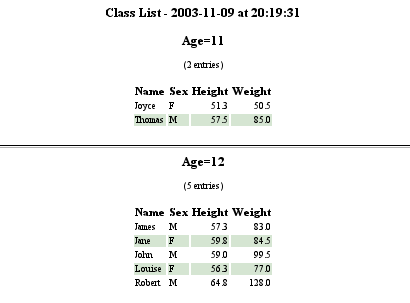
\includegraphics[width=5in]{ages2.png}
\end{goutput}

\subsection{various problems}
\index{Events!table\_head}
\index{Style!table\_head}
The first time this job runs, there is a warning in the log that the table\_head style
was not found.  This is coming from the stripes tagset where the table\_head event
is asking for the table\_head style.  It doesn't really cause any problems but defining
an empty style will take care of the warning.

\begin{sfvcode}
   style table_head
   ;
\end{sfvcode}
 
The other thing that is needed is a style for the number of observations label.  The style has
now grown to look like this.

\begin{fvcode}{datastep_style}{Refined striped style}
    define Style styles.minimal_striped; 
        parent = styles.minimal;

        style header/
            font = (, 4,bold)
        ;

        style Data/
            font = (, 3,normal)
        ;

        style DataStrong from data /
            background=cxD5E5D2
        ;

        style nobs_label from data /
        ;

        style table_head
        ;

        style byline /
           font_size = 5
           font_weight = bold
        ;

        replace Output /
            BorderWidth = 0
            CellSpacing = 1
            CellPadding = 7
            Frame = void
            Rules = none
        ;

    end;
\end{fvcode}


\subsection{Modifying the Byline}
\index{Byline!modification}
All that is left is for the byline to modified to match what the datastep code did.
This part isn't too hard either.  The easiest way to do this is to code it for the
data we are reporting on.  That makes this tagset specific to the task, and not
very reusable.  But it is a good first step.

\index{Variables!Macro}
\index{Events!Nobs\_label}
\index{Events!Byline}
Another option will work nicely to indicate which byline needs to be modified. Luckily
only one by value needs changing.  The end of the byline can be postponed until the 
table ends.  That means that the nobs event from the nobs\_count tagset can handle most 
of the work.  In the interest of versatility the byline and nobs\_label events have
been set up to work together.  If there is no byline, the nobs\_label event handles
the situation by doing the setup that the byline event would have done if there was a byline.

The new tagset and it's output follows.

\begin{fvcode}{by_age_tagset}{Tagset with modified by lines}
    define tagset tagsets.by_age;
        parent=tagsets.nobs_label;
        
        /*-------------------------------------------------------eric-*/
        /*-- Add some extra comments to the doc event.              --*/
        /*----------------------------------------------------8Aug 03-*/
        define event initialize;
            unset $do_nobs;
            do /if $options;

                do /if $options['MODIFY_BY'];
                    eval $modify_by inputn($options['MODIFY_BY'], '7.');
                    do /if missing($modify_by);
                        eval $modify_by 0;
                    done;
                done;

                set $do_nobs "true" /if cmp($options['NOBS_LABEL']), 'yes');

                /*---------------------------------------------------eric-*/
                /*-- From the stripes tagset.                           --*/
                /*------------------------------------------------9Nov 03-*/
                set $alt_row_style $options['ALTERNATE_STYLE']";
            done;

            set $alt_row_style 'DataStrong' /if !$alt_row_style;

        end;    


        /*-------------------------------------------------------eric-*/
        /*-- We want to say two different things depending on the   --*/
        /*-- value in the byline.                                   --*/
        /*----------------------------------------------------7Aug 03-*/
        define event byline;
            /*---------------------------------------------------eric-*/
            /*-- Convert age to a numeric.                          --*/
            /*------------------------------------------------7Aug 03-*/
            eval $byval inputn(scan(value, -1, '='), '7.');
        
            put '<p><div';
            putq ' class=' htmlclass ;
            put ' style="text-align: center;">' nl;

            do /if $byval = $modify_by ;
                put 'The Oldest';
            else;
                put 'Age is ' $byval ;
            done;
            
            /*---------------------------------------------------eric-*/
            /*-- A newline would do, but one way or another we need --*/
            /*-- to flush.  Otherwise the timing goes sour.         --*/
            /*------------------------------------------------8Aug 03-*/
            flush;
            set $byline "true";
        end;
        

        /*-------------------------------------------------------eric-*/
        /*-- The nobs title finishes up the paragraph started with  --*/
        /*-- the byline.                                            --*/
        /*----------------------------------------------------7Aug 03-*/
        define event table_nobs_label;
            style=nobs_label;

            /*---------------------------------------------------eric-*/
            /*-- If we did not get a byline then we want to make    --*/
            /*-- sure the html is still well formed.                --*/
            /*------------------------------------------------8Aug 03-*/
            do /if ^$byline;
                put '<p><div';
                putq ' class="byline"';
                put ' style="text-align: center">' nl;
                unset $byline;
            done;

            put '&nbsp;&nbsp;<span class="' htmlclass '">(' $nobs ' ';

            do /if $nobs = 1; 
                put 'entry)' ;
            else;
                put 'entries)' ;
            done;

            put '</span></div></p>' nl;
        end;

    end;
\end{fvcode}

The proc print that creates this output is still rather simple.  Only the two
macro variables look out of the ordinary.

\begin{sfvcode}
title;

ods tagsets.by_age options(nobs_label='yes' modify_by='16')
    file="ages3.html" (title='Class List')
    style=minimal_striped;

proc sort data=sashelp.class out=myclasssrt;
  by age name sex height weight;
run;

*options obs=6;

proc print data=work.myclasssrt noobs;
    by age;
    pageby age;
run;

ods tagsets.by_age close;
\end{sfvcode}


\begin{goutput}{ages3_out}{Output with modified By lines}
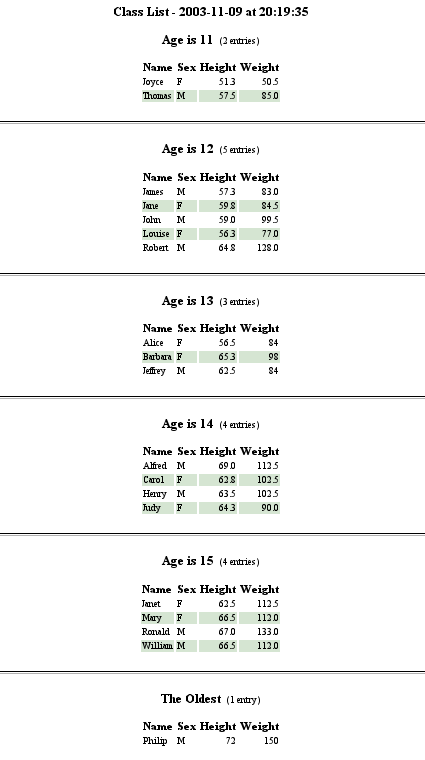
\includegraphics[width=4in]{ages3.png}
\end{goutput}

\subsection{A more flexible solution}
\index{Events!Byline}
\index{Dictionary}
This tagset is simple enough that it doesn't really matter that it's specific to this
data.  But with a little work it can be made more universal.  All it needs is a more
flexible way to indicate which by values need reformatting, and what they should be 
reformatted to.  That can be done with a macro variable. The heart of this tagset
is a dictionary.  When the proc starts the macro variable is parsed and put in 
the dictionary.  The byline event uses the dictionary to decide what to do with
each byline.  

\index{Events!Bygroup}
\subsubsection{More Identify, and Locate}
\index{ByLines}
There is an event called bygroup that surrounds all bygroup processing.  Using the start
of that event to parse the macro variable and set up the by value dictionary for the by lines
that will be coming. All of this requires that the by values are known.  But that
was a prerequesite for this particular problem anyway.

The new mod\_by\_line tagset follows.

\begin{fvcode}{flexible_byline_tagset}{A more versatile byline tagset}
 define tagset tagsets.mod_by_line;
        parent=tagsets.nobs_label;
        
        define event bygroup;
            start:
                /*-----------------------------------------------eric-*/
                /*-- Do not do this if there is no need.            --*/
                /*--------------------------------------------9Nov 03-*/
                break /if ^modify_by;

                break /if cmp($modify_by, modify_by);
                
                unset $byval_subs;
                set $modify_by modify_by;
                
                eval $count 1;
                trigger set_byval_pair;

                do /while !cmp($byval_pair, ' ');

                    set $byval_subs[$byval] $substitution;

                    eval $count $count+1;

                    trigger set_byval_pair;
                done;

        end;

        define event set_byval_pair;     
            set $byval_pair scan($modify_by, $count, '|');
            set $byval scan($byval_pair, 1, ':');
            set $substitution scan($byval_pair, 2, ':');
        end;   
        

        define event byline;
            /*---------------------------------------------------eric-*/
            /*-- Get the by value in string form                    --*/
            /*------------------------------------------------7Aug 03-*/
            eval $byval trim(scan(value, -1, '='));
            
            put '<p><div';
            putq ' class=' htmlclass ;
            put ' style="text-align: center;">' nl;

            do /if $byval_subs[$byval];
                put $byval_subs[$byval];
            else;
                do /if by_label;
                    put by_label $byval;
                else;
                    put value;
                done;
            done;
            
            /*---------------------------------------------------eric-*/
            /*-- A newline would do, but one way or another we need --*/
            /*-- to flush.  Otherwise the timing goes sour.         --*/
            /*------------------------------------------------8Aug 03-*/
            flush;
            set $byline "true";
        end;
        

        define event table_nobs_label;
            style=nobs_label;

            /*---------------------------------------------------eric-*/
            /*-- If we did not get a byline then we want to make    --*/
            /*-- sure the html is still well formed.                --*/
            /*------------------------------------------------8Aug 03-*/
            do /if ^$byline;
                put '<p><div';
                putq ' class=' htmlclass;
                put ' style="text-align: center">' nl;
                unset $byline;
            done;

            put '&nbsp;&nbsp;<span class="' htmlclass '">(' $nobs ' ';

            do /if $nobs = 1; 
                put 'entry)' ;
            else;
                put 'entries)' ;
            done;

            put '</span></div></p>' nl;
        end;

    end;
\end{fvcode}

\index{Debugging}
\index{Putlog}
\index{Statements!Putlog}
\index{Putvars}
\index{Statements!Putvars}
Tagsets like this are not all that difficult except that a mis-spelled variable or
an incorrect if statement will cause it to quietly not do what you asked.  A well placed
putlog or putvars statement can be very revealing.  In this case checking for
the options and memory variables looks like this.

\begin{sfvcode}
   putvars $options _name_ ':' _value_ ':' nl;
   putvars mem _name_ ':' _value_ ':' nl;
   putvars $byval_subs _name_ ':' _value_ ':' nl;
\end{sfvcode}

There are two things in these examples that help with debugging.  The placement
of a character on both sides of a value to reveal whitespace.  The other trick
is to separate the highly visible label from the variable by inserting another
string between them.  Then if the variable does not exist, the label will still
print.

\index{Variables!Macro}
The new job which uses the new macro variables is shown in the following job 
which creates the output in figure \ref{ages4_out} on page \pageref{ages4_out}.

\begin{sfvcode}
title;

ods tagsets.mod_by_line 
    options(nobs_label='yes' 
            by_label='Age is' 
            modify_by='16:The Oldest|11:The Youngest')
    file="ages4.html" (title='Class List')
    style=minimal_striped;

proc sort data=sashelp.class out=myclasssrt;
  by age name sex height weight;
run;

proc print data=work.myclasssrt noobs;
    by age;
    pageby age;
run;

ods tagsets.mod_by_line close;
\end{sfvcode}

\begin{goutput}{ages4_out}{Modifying Bylines, Final output}
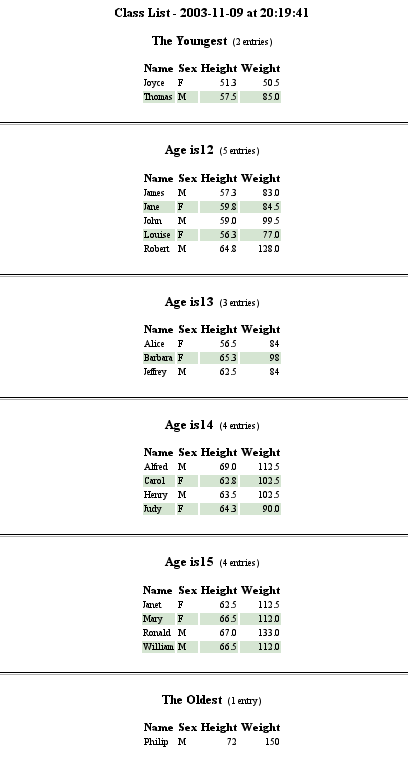
\includegraphics[width=4in]{ages4.png}
\end{goutput}


\section{Summary}
This chapter has shown some of the advantages of converting datastep code
to tagsets.  Tagsets do not pretend to replace datastep, but if responsiblities
are divided between datastep and tagsets then the solution is more open for 
re-use in later solutions.  More power and flexibility is also provided by the
tight integration the output now has with ODS.


%%\cleardoublepage

%\part{Advanced Examples}
%{
%These chapters will cover more advanced examples.  These examples are
%more advanced because they do more than one thing at a time.  Multiple
%concepts are needed to accomplish these solutions.  These chapters will
%cover website integration, Data Step Conversions, repeating headers, 
%automatic paneling of output, and an extension of the slidebar example shown earlier.
%Understanding these examples is a good indication that all problems are within
%your grasp. 
%}

%%\chapter{ODS Output for Website Integration}
\index{Website Integration}
\index{Website Templates}
Many web sites have a framework that web pages must fit into 
before they will be published.  Usually this means
editing the html pages and pasting in some chunk of HTML from
some files the website authors have provided.
Usually there is one file to replace the top section of the
web page and another to replace the bottom.  
The tagsets in this chapter will create HTML that
is ready for integration with any website.  

\section{The Problem}
Most websites want webpages to be enclosed with some sort of
image and navigation menu at the top and/or bottom.  Most of this
is usually enclosed in some sort of table to control the layout.

This enclosing HTML is usually put in two files so that it is easy
to include them as the top and bottom of each web page.  Prior to
SAS 9.1 there were two ways to do this.  The hardest way is to use
the no\_top and no\_bot options along with some datastep to write
the file templates.  Starting with SAS 8.2 it became possible to
create a tagset that included the text from the website's framework
files.  This is really the simplest way to do this, but it leads
to dual maintenance because everytime the files change, the tagset
needs to have the same changes.

\index{Website Integration}
\index{Website Templates}
\index{Statements!Putl}
\index{Putl}
If that is the route you wish to take there is a put command that
will help.  'Putl' is just like put except that it has an automatic
newline at the end.  That means you can copy and paste in a block
of text and place a putl ' at the beginning and a '; at the end of
each line.  That's not too hard but can be painful if the framework
files change very often.

The framework files usually include everything that goes in an HTML
document down to and including the body tags.  All of your content
goes inbetween with no need to define the basic HTML document.  At
the very least the solution needs to eliminate the output from the
events above the start and below the finish of the doc\_body event.

The most difficult part of this is that somehow, the stylesheet for
the ODS output will have to be incorporated into the middle of the
framework text.  If your web designers are nice, they may be willing
to place an ods generated stylesheet with their other stylesheets.
They may even put a reference to it in their framework file.  In
that case the tagset will be easy.  Either way, a working tagset
can be created.

\section{Alternate Behavior for existing options}
The first step towards this solution is to eliminate all the events
above and below the body tags.  ODS already gives options to do
that.  All that is needed is to detect when those options are set.
Then detect if there are files that can be used in place of the
head and foot sections of the document.

\index{Options!No\_Top\_Matter}
\index{Options!No\_Bottom\_Matter}
\index{Options!No\_Top}
\index{Options!No\_Bot}
\index{Variables!No\_Top}
\index{Variables!No\_Bot}
Macro variables, or alias can be used to specify the files to read.
If both the no\_top\_matter and no\_bottom\_matter options are used
with file name specifications, then the tagset can behave as desired.
Otherwise normal behavior will be the way to go.

\subsection{Explore}
Running an event map with the notop and nobot options shows that there are variables in
the tagset called no\_top and no\_bot that indicate these options were set.  That will
be very useful.

\index{Events!Initialize}
The trick to this tagset is using the initialize event to advantage.  The initialize
event always happens.  But when no\_top and no\_bot is used the first and last events
are somewhat variable.   The first event could be system\_titles, or not.  The last could
be system\_footers, or not.  Reviewing the available events shows that no\_bot causes
the end to be unpredictable.  Luckily there are not that many events in the bottom
section of an html document.  As usual, the initialize event can be used to set things up, and
redefine the events in the bottom section to do the right thing.  That means that
all the external controls need is the no\_top option with some method of passing two 
filenames to read.

\section{Reading an external file}

\index{Functions!filename}
\index{Functions!fopen}
\index{Functions!fread}
\index{Functions!fget}
\index{Functions!Return Code}
\index{Statements!Eval}
\index{Statements!Set}
\index{DataStep!Functions}
The key to this tagset is reading an external file.  That example is shown
on page \pageref{readfile}.  This example will build on that functionality.

Your website's authors will probably have two files that may resemble the following
HTML code.  The top section defines the html document and starts the body section
of the page and creates some tables for layout.  There is a table along the top for
the Company logo and navigation.  Below that is another table with one row and three
cells.  The first cell contains another table with more navigation menus.  the second
cell is where The sas output will go.  The second file closes everything up, puts a
table across the bottom for more navigation, contacts, copyright notices and the like.

\begin{Verbatim}[frame=lines, framesep=3mm, label={Sample}]

<!DOCTYPE html PUBLIC "-//W3C//DTD XHTML 1.0 Transitional//EN"
    "http://www.w3.org/TR/xhtml1/DTD/xhtml1-transitional.dtd">

<html xmlns="http://www.w3.org/1999/xhtml">
  <head>
    <meta name="generator" content="HTML Tidy, see www.w3.org" />
    <meta content="text/html; charset=iso-8859-1"
    http-equiv="Content-Type" />

    <title>Your website name</title>
    <meta name="description" content="Your website name" />
    <meta name="keywords" content="SAS, ODS, Markup, HTML, XML" />

    <link rel="shortcut icon" href="/favicon.ico" type="image/x-icon" />
    <link rel="icon" href="/fav_icon.ico" type="image/x-icon" />
    <style type="text/css">
    <!--
    .main{Background-color:#E0E0E0;
          color:#000000;
         }

    a:link { color:#0066AA }
    a:visited { color:#004488 }
    a:active { color:#004488 }

    .layout_table{cellspacing: 0;
                  padding: 0;
                  borderwidth: 0px;
                  width: 100%;
         }
    .nav_table{cellspacing: 0;
                  borderwidth: 0px;
                  width: 50px;
                  background-color: #00DD55;
         }
    .nav_label{color: #000088;
               font-size: medium;
               font-weight: bold;
         }
    .output_cell{color: #E0E0E0;
         }
    </style>
  </head>

  <body class="main">

    <!-- Beginning of Top headline and navigation table -->
    <table class="layout_table">
      <tr>
        <td><a href="http://www.yourdomain.org/index.html">
        <img src="gifs/logo.gif" height="94" width="306"
        alt="Logo Image alt text: Your Company: Slogan" border="0" /></a>
        </td>

        <td align="right" valign="bottom">

          <form action="http://www.yourdomain.org/cgi/region.cgi"
          method="get">
            <br />
            <span class="nav_label">Select your Region:</span>
            <br />
            <select name="goto">
              <option value="http://www.yourdomain.org/region1"> Region 1 </option>

              <option value="http://www.yourdomain.org/region2">
                Region 2
              </option>

              <option value="http://www.yourdomain.org/region3">
                Region 3
              </option>

              <option value="http://www.yourdomain.org/region4">
                Region 4
              </option>

              <option value="http://www.yourdomain.org/region5">
                Region 5
              </option>

              <option value="http://www.yourdomain.org/region6">
                Region 6
              </option>
            </select><input type="submit" value=" Go " /><br />

          </form>
        </td>
      </tr>
    </table>
    <hr size="1" noshade="noshade" />

    <!-- Beginning of main table -->
    <table class="layout_table">
      <tr>

        <!-- Beginning of Left Side Navigation Bar. -->
        <td valign="top">
          <table class="layout_table">
            <tr>
              <td>
                <table class="nav_table">
                  <tr>
                    <td>
                      <p><font class="nav_label"><b>News</b></font>
                      <small><br />

                       <a href="news/newsflash.html">Announcements</a><br />

                       <a href="news/press.html">In the Press</a><br />
                       <a href="news/index.html">More ...</a>
                       </small></p>

                      <p><font class="nav_label"><b>Company</b></font>
                      <small><br />

                       <a href="./contact/index.html">Contact Information</a><br />
                       <a href="./about/index.html">About</a><br />
                      </small></p>

                      <form action="http://www.yourdomain.org/cgi/search.cgi"
                       method="get">

                        <small>Search for:<br />
                        <input type="text" name="words" size="10" />
                        <input type="hidden" name="max" value="25" />
                        <input type="hidden" name="source" value="www" />
                        <input type="submit" value="Go" />
                        </small>
                      </form>
                    </td>
                  </tr>
                </table>
              </td>
            </tr>

          </table>
        </td>
        <!-- End of Left Side Navigation Bar. -->

        <!-- Beginning of Center - Output Panel -->
        <td class="output_cell">
\end{Verbatim}

The ending of your website's pages may look something like this

\begin{Verbatim}[frame=lines, framesep=3mm, label={Sample2}]
        </td>
        <!-- End of Center - OutputPanel -->

        <!-- beginning of Right - Navigation Panel -->
        <td align="right">
           <table class="nav_table" >
             <tr><td>
               <ul>
                 <li> More Navigation:</li>
                 <ul>
                   <li> Navigation1</li>
                   <li> Navigation2</li>
                 </ul>
               </ul>
             </td></tr>
           </table>
        </td>
        </tr>
    <!-- End of Middle - Layout table -->
   </table>

   <table class="layout_table" >
   <tr>
   <td align="center">
    <hr size="1" noshade="noshade" /><br/>
       Copyright 2004 Your Company name. 
   </td>
   </tr>
   </table>

</body>
</html>
\end{Verbatim}

\section{The Solution}
The following tagset will read the files given through the tagset alias or 
a macro variable called infiles.  Alias or infiles should be two
filenames separated by a space.   
If tagset alias is set to 'default' then the 
set\_default\_files event is used to set the default file names.
By using a separate event, this tagset can be used as a parent
tagset, where only the set\_default\_files event is redefined.
This also allows normal no\_top behavior if no files are specified.  

Another key to this tagset is that only external stylesheets are
allowed.  It is possible to make embedded stylesheets work.  But
that behavior is not really desirable in this case because our network
administrators wouldn't like embedded stylesheets in our files.  
A stylesheet file must be specified on the ods statement when using
this tagset.

\subsection{Initialization Timing}
\index{Tagsets!short\_map}
\index{Events!Proc}
\index{Events!Initialize}
\index{Events!Initialize!Timing}
\index{Files!Stylesheet}
\index{Variables!No\_Top}
Upon trying this method with the stylesheet option, it can be seen that the initialize event
doesn't work quite right.  That's because initialize happens once.  At the very beginning.
The stylesheet file is created before the body file, so that's when it happens.  No\_top isn't
set for the stylesheet, so the head section of the body file is never printed.  
The solution can be found
by running the same output through the short\_map tagset - with the same ods statement options.
What can be seen is that the proc event always comes out the first thing.  Using the first
proc event to print the top of the file template will work just fine.
 
The best solution is for the website's templates include an ods stylesheet. 
In that case specifying a stylesheet on the ods statement won't be 
necessary.  That would also insure that all ODS output always matches
the website.  All things considered this is still a fairly simple tagset.  The
most complex parts are the things that make it work invisibly for users
who don't want or need this special behavior.

\begin{fvcode}{Web_integration}{Website integration Tagset}
/*----------------------------------------------------------------*/
/*-- Reading a file in using datastep functions.  This example  --*/
/*-- comes straight out of the online documentation             --*/
/*-- for fread().                                               --*/
/*----------------------------------------------------------------*/
proc template;
    define tagset tagsets.website;
        parent=tagsets.html4;
        embedded_stylesheet=no;

        define event initialize;

            do /if $options;
               do /if $options['HEAD_FILE']; 
                   set $head_file $options['HEAD_FILE'];
               done;
               do /if $options['FOOT_FILE']; 
                   set $foot_file $options['HEAD_FILE'];
               done;
               do /if cmp($options['DEFAULT_FILES'], 'yes'); 
                    set $head_file 'default_head.html' /if ^$head_file;
                    set $foot_file 'default_foot.html' /if ^$head_file;
               done;
            done;

            putlog "Infiles are" " :" $head_file "  " $foot_file;

            set $filename $head_file;

            /*--------------------------------------------eric-*/
            /*-- Set a flag so the ending document tags      --*/
            /*-- can be suppressed.                          --*/
            /*-----------------------------------------8Nov 03-*/
            do /if $infiles);
                set $read_files 'true';
                set $filrf "headfile";
                set $read_head "true";
            done;
        end;

        define event proc;
            start:
                do /if no_top;
                    do /if $read_head;
                        trigger readfile;
                        unset $read_head;
                    done;
                done;
        end;


        define event head_search;
            trigger integrated_link /if contains($file_record, '</head>');
        end;

        define event integrated_link;
            put '<style type="text/css">' CR '<!--' CR;
            trigger alignstyle;
            put '-->' CR '</style>' CR ;
        
            set $urlList stylesheet_url;
            set $urlList stylesheet_name /if !$urlList;
            trigger urlLoop ;
            unset $urlList;
        end;

        define event readfile;
            
            /*------------------------------------------------*/
            /*-- Set up the file and open it.               --*/
            /*------------------------------------------------*/
            putlog "Reading in file: " $filename;

            eval $fid 0;
            
            eval $rc filename($filrf, $filename);
            
            eval $fid fopen($filrf);
            do /if missing($fid);
                putlog "Error: Could not open file, " $filename;
                break;
            done;


            /*---------------------------------------------------*/
            /*-- datastep functions  will bind directly to the --*/
            /*-- variable space as it exists.                  --*/
            /*--                                               --*/
            /*-- Tagset variables are not like datastep        --*/
            /*-- variables but we can create a big one full    --*/
            /*-- of spaces and let the functions write to it.  --*/
            /*--                                               --*/
            /*-- This creates a variable that is 200 spaces so --*/
            /*-- that the function can write directly to the   --*/
            /*-- memory location held by the variable.         --*/
            /*-- in VI, 200i<space>                            --*/
            /*---------------------------------------------------*/
            set $file_record  "

                                  ";

            /*-------------------------------------------------*/
            /*-- Loop over the records in the file           --*/
            /*-------------------------------------------------*/
            do /if $fid > 0 ;

                do /while fread($fid) = 0;

                    set $rc fget($fid,$file_record ,200);

                    trigger head_search;
                    
                    /* trimn to get rid of the spaces at the end. */
                    put trimn($file_record ) nl;

                done;
            done;

           /*----------------------------------------------------*/
           /*-- close up the file.  set works fine for this.   --*/
           /*----------------------------------------------------*/

            set $rc close($fid);
            set $rc filename($filrf);

        end;

        define event doc;
            start:
                set $doctype '<!DOCTYPE html PUBLIC "-//W3C//DTD HTML 4.01 Transitional//EN">';
                set $framedoctype '<!DOCTYPE html PUBLIC "-//W3C//DTD HTML 4.01 Frameset//EN">';
                put $doctype CR;
                put "<html>" CR;

            finish:
                do /if $read_files;
                    set $filename scan($infiles, 2, ' ');
                    set $filrf "footfile";
                    trigger readfile;
                    break;
                done;

                put "</html>" CR;
        end;

        define event doc_body;
            put '<body onload="startup()"';
            put ' onunload="shutdown()"';
            put  ' bgproperties="fixed"' / WATERMARK;
            putq " background=" BACKGROUNDIMAGE;
               trigger style_inline;
            put ">" CR;
            trigger pre_post;
            put          CR;
            trigger ie_check;

          finish:
            trigger pre_post;

            break /if $read_files;
            put "</body>" CR;
        end;

end;

run;


ods tagsets.shortmap stylesheet="stylesheet.map" 
                          file="website.map"(notop) ;

ods tagsets.website stylesheet="website.css" 
                          file="website.html"(notop) 
                         options(default_files = 'yes');

proc print data=sashelp.class; run;
    
ods tagsets.website close;
ods _all_ close;
\end{fvcode}

\section{Summary}
\index{Website Integration}
The output using these particular template files is shown 
in figure \vref{website_out}.  
Working with the authors of your website should enable you to create some very
nice looking output.  All of which is immediately ready for integration.
        
\begin{goutput}{startpage2_out}{Website integration}
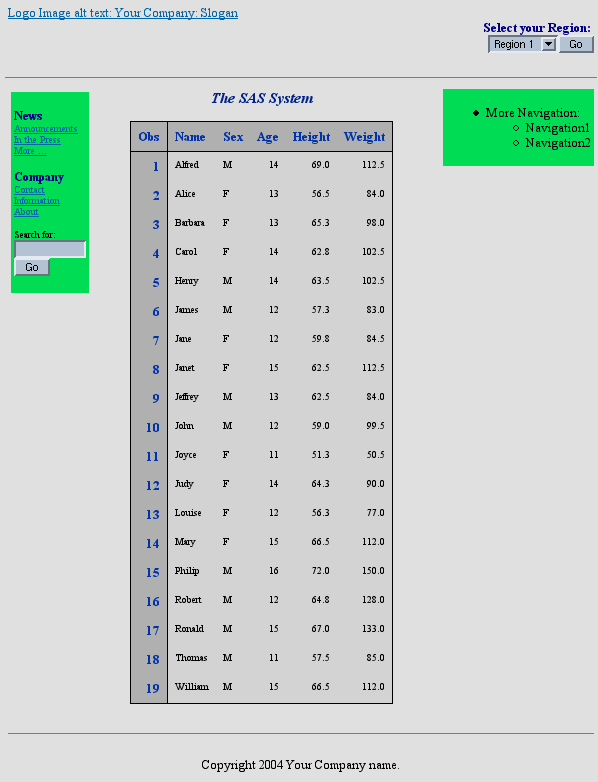
\includegraphics[width=6in]{website.png}
\end{goutput}

%%\cleardoublepage
%%\chapter{Datastep Conversions}
\index{DataStep Conversions}
You may wonder, why would someone want to convert a datastep 
program to use tagsets?  There are lots of reasons.  Mostly it's
for code reuse and flexibility.  Datastep programs allow lots of
flexibility but they are written for one purpose.  If the same 
functionality is desired for a different set of data an entirely
new datastep will have to be written.  If the rendering is left to
a tagset, then anyone can use that tagset with any form of data,
and any procedure.  Maintenance of the code is also simplified 
since both the tagset and the resulting SAS job wil be much
simpler than the original datastep. Add the various powers of
ODS to this new found flexibility and there is plenty of motivation
for conversion.  This chapter will show the process and rewards 
of converting datastep programs to tagsets. 

\index{DDE}
\index{CSV}
\index{XML}
Yet another reason to
convert is that tagsets can be interchanged to create new and 
diffrent outputs.  Usually datastep is used to create HTML, CSV,
or DDE to XML,  A different datastep is required for each.  A different
tagset is required for each as well.  The difference is the reusability
and the ease of creation and maintenance.

\index{ODS}
\index{ODS!Styles}
\index{ODS!Select}
\index{ODS!Exclude}
\index{ODS!Document}
Full integration with ODS provides more than enough reasons to convert 
a datastep to a tagset.  Ods styles, table templates, select and exclude,
and proc document are very good reasons.  There are many other things that
ODS can do besides these, but not if datastep is the method of creating the
output.

\section{Special Bylines}
\index{nobs}
\index{Counting Observations}
\index{Bylines}
One of the things that can be done in datastep is the counting of observations
for display in the byline.  The datastep just counts them first then another
datastep prints everything out.  Tagsets can do that too.  This first example
has a special style, as well as a special byline.  The byline text may change
based upon the current by value.  Each byline also displays the number of
observations in the table below it.  

\subsection{The DataStep Code}
\index{Procedures!Report}
\index{Highlighting}
The original datastep code is shown below.  It has been simplified to use
the sashelp.class dataset.  There is nothing very hard about this code.  The
worst thing is all the puts.  The original data step also did some highlighting
and value translation.  Both of those things are much easier to do using the report procedure.
Another nice thing this datastep does is put the web page title in the title tag and
as the heading on the page.  This is also easy to do with a tagset. The original
output can be seen in figure \vref{ages_out}.

\begin{sfvcode}
filename webout 'ages.html';

%let numfuture=16;

proc sort data=sashelp.class out=myclasssrt;
  by age name weight;
run;

/* Count number of items in each BY group */
data cnt_by_obs;
   keep cnt;

   set work.myclasssrt;
   by age;

   if first.age then curcnt = 0;
   curcnt + 1;
   if last.age then do; cnt = curcnt; output; end;
run;

options missing='-';
data _null_;
   file webout;
   if _N_ = 1 then do;
      length title $ 128;
      length stoday stime $ 8;
      retain linecnt 1;

      stoday = put( today(), date7. );
      stime = put( time(), time5. ); 
      title = 'Class List &nbsp;-&nbsp; ' || stoday || "at " || stime;
      put '<!DOCTYPE HTML PUBLIC "-//IETF//DTD HTML//EN">';
      put '<HTML><HEAD>';
      put '<TITLE>' title '</TITLE>';
      put '</HEAD><BODY>';
      put '<CENTER><H3>' title '</H3></CENTER>';
   end;

   set work.myclasssrt;
   by age;

   if _N_ = 1 or FIRST.age then do;
      length lab $ 32;
      set work.cnt_by_obs;
      if age >= &numfuture then do;
         put '<CENTER><B><FONT SIZE=+2>The Oldest</FONT> ' @;
         put '<FONT SIZE=-1>(' cnt +(-1) ' '@;
         if cnt = 1 then
            put 'entry)' @;
         else
            put 'entries)' @;
         put '</FONT></B></CENTER>';
      end;
      else do;
         put '<CENTER><B><FONT SIZE=+2>Age is ' age '</FONT> ' @;
         put '<FONT SIZE=-1>(' cnt +(-1) ' '@;
         if cnt = 1 then
            put 'entry)' @;
         else
            put 'entries)' @;
         put '</FONT></B></CENTER>';
      end;
      put '<TABLE ALIGN=CENTER VALIGN=MIDDLE>';
      put '<TR>';
      lab = vlabel(Name);         put '<TH>' lab '</TH>';
      lab = vlabel(Weight);       put '<TH>' lab '</TH>';
      lab = vlabel(Height);       put '<TH>' lab '</TH>';
      lab = vlabel(Sex);          put '<TH>' lab '</TH>';
      put '</TR>';
   end;

   if mod(linecnt,2) then
      put '<TR ALIGN=CENTER VALIGN=MIDDLE BGCOLOR="D5E5D2">';
   else
      put '<TR ALIGN=CENTER VALIGN=MIDDLE>';

   put '<TD ALIGN=CENTER>' name '</TD>';
   put '<TD><FONT SIZE=-1>' weight '</FONT></TD>';
   put '<TD><FONT SIZE=-1>' height '</FONT></TD>';
   put '<TD><FONT SIZE=-1>' sex '</FONT></TD>';
   put '</TR>';

   linecnt + 1;

   if LAST.age then do;
      put '</TABLE>';
      linecnt = 1;
      put '<BR><HR><BR>';
      put '</BODY></HTML>';
   end;
run;

\end{sfvcode}

\begin{goutput}{ages_out}{Data step}
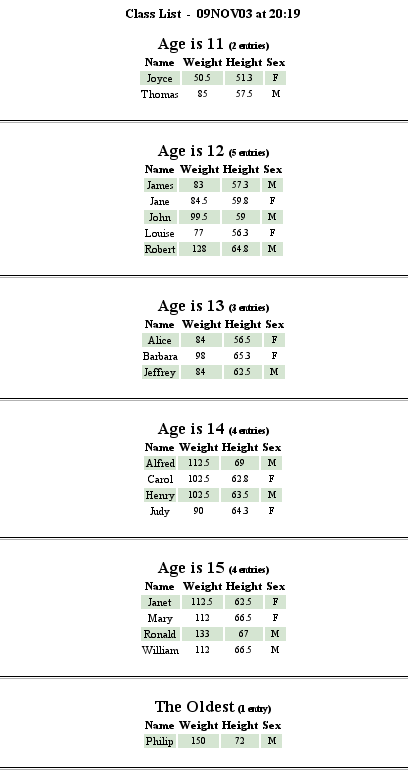
\includegraphics[width=4in]{ages.png}
\end{goutput}


\subsection{Breaking it down}
\index{Styles!Minimal}
The best way to approach a problem like this is to break it down into separate
problems.  In this case there is a fairly minimalist set of colors and fonts.
A fairly simple ODS style can be created from what can be seen in the datastep code.

\index{Tables!striping}
The next problem is striping of tables.  That problem was solved in the example on
page \pageref{striped_table}.
So this new tagset can use the stripes tagset as it's parent.  

\index{Byline!Modifying}
\index{Counting Observations}
There are three more things to solve, Extending the use of the title, counting the 
observations, and modifying the byline.  It would be perfectly
reasonable to solve both those problems in one tagset.  But the last
tagset is simpler if an
intermediate tagset is created to count the observations and display the count.
As a bonus the intermediate tagset can be used in other jobs to solve
other problems because it is not specific to this specific problem.

\subsection{The Style}
\index{Styles!Minimal}
Extracting all the colors and fonts from the datastep is easy enough.  
With something this simple the best thing is to use the minimal style as
a parent.  The minimal style will provide everything that is needed 
without making things complicated.
The resulting style looks like this.

\begin{sfvcode}
    define Style styles.minimal_striped; 
        parent = styles.minimal;

        style header/
            font = (, 4,bold)
        ;

        style Data/
            font = (, 3,normal)
        ;

        style DataStrong from data /
            background=cxD5E5D2
        ;

        replace Output /
            BorderWidth = 0
            CellSpacing = 1
            CellPadding = 7
            Frame = void
            Rules = none
        ;

    end;
\end{sfvcode}


\subsection{Counting Observations}
\index{Observation Count}
\index{Number of Observations}
\index{nobs}
\index{Variables!Macro}
The new tagset inherits from tagsets.stripes from page \pageref{striped}. 
This tagset manipulates the title and prints it as a heading. 
We also add a counter for the observations, and a stream to catch
the table while the observations are being counted.  The last thing is to add
an event to print the observation count.
A macro variable called do\_nobs\_label must be set to 'true' for the observation
counting to take effect.  Otherwise the tagset will exhibit normal behavior.
This tagset will work for any tabular output that ods creates.  
The new tagset looks like this.  
The Output is shown in listing \vref{ages2_out}.

\begin{sfvcode}
proc template;
    define tagset tagsets.nobs_label;
        parent=tagsets.stripes;

        define event initialize;
            unset $do_nobs;
            do /if $options;

                set $do_nobs "true" /if cmp($options['NOBS_LABEL']), 'yes');

                /*---------------------------------------------------eric-*/
                /*-- From the stripes tagset.                           --*/
                /*------------------------------------------------9Nov 03-*/
                set $alt_row_style $options['ALTERNATE_STYLE']";
            done;

            set $alt_row_style 'DataStrong' /if !$alt_row_style;
        end;    

        define event options_set;
            trigger initialize;
        end;

        /*-------------------------------------------------------eric-*/
        /*-- Add the date and time to the document title.  Save it  --*/
        /*-- away for later.                                        --*/
        /*----------------------------------------------------7Aug 03-*/
        define event doc_title;
              break /if ^value;
              set $title value '&nbsp;-&nbsp;' date " at " time; 
              putl '<TITLE>' $title '</TITLE>';
        end;

        define event doc_body;
            start:
                put '<body onload="startup()"';
                put ' onunload="shutdown()"';
                put  ' bgproperties="fixed"' / WATERMARK;
                putq " class=" HTMLCLASS;
                putq " background=" BACKGROUNDIMAGE;
                trigger style_inline;
                put ">" nl;
                trigger pre_post;
                put          nl;
                trigger ie_check;

                /*-----------------------------------------------eric-*/
                /*-- This is the part that changed.                 --*/
                /*-- Add in the title if we have one.               --*/
                /*--------------------------------------------7Aug 03-*/
                do /if $title;
                    putl '<h3';
                    trigger align;
                    putl '>' $title '</h3>';
                done;

            finish:
                trigger pre_post;
                put "</body>" nl;
        end;

        define event output;
            finish:
                put "<br>" nl;
        end;

        define event table ;
            start:
                eval $nobs 0;
                
                /*-----------------------------------------------eric-*/
                /*-- if we are not going to print the nobs label   --*/
                /*-- then there is no point in doing extra work.   --*/
                /*--------------------------------------------7Aug 03-*/
                open table /if cmp($do_nobs, 'true');
                set $row_class 'data';
                
                put "<div";
                trigger alt_align;
                put ">" CR;
                put '<table>' nl;
            finish:
                put '</table>' nl;
                put "</div>" nl;
                
                /*-----------------------------------------------eric-*/
                /*-- if we are not going to print the nobs label   --*/
                /*-- then there is no point in doing extra work.   --*/
                /*--------------------------------------------7Aug 03-*/
                do /if cmp($do_nobs, 'true');
                    close;
                    /* print the nobs */
                    trigger table_nobs_label; 

                    /* print the table */
                    put $$table;
                    unset $$table;
                done;
        end;
        
        /*-------------------------------------------------------eric-*/
        /*-- Count the data rows.  Swap colors.                     --*/
        /*----------------------------------------------------7Aug 03-*/
        define event row;
            start:
                /*-----------------------------------------------eric-*/
                /*-- Don not count unless we are in the data.       --*/
                /*--------------------------------------------7Aug 03-*/
                putq '<tr>' nl;
                do /if cmp(section, 'body');
                    eval $nobs $nobs+1 ;
                done;
            finish:
                put '</tr>' nl;
                /*-----------------------------------------------eric-*/
                /*-- Swap the row style at the end of the row.      --*/
                /*-- That way the first row is the one we set in    --*/
                /*-- table start.                                   --*/
                /*--------------------------------------------7Aug 03-*/
                trigger swapclass /if cmp(section, 'body');
        end;
        

        /*-------------------------------------------------------eric-*/
        /*-- Print a small heading above the table.                 --*/
        /*-- (## entries)                                           --*/
        /*----------------------------------------------------7Aug 03-*/
        define event table_nobs_label;
            style=nobs_label;
            put '<p><h4';
            putq ' class=' htmlclass; 
            put ' style="text-align: center">(' $nobs ' ';
            do /if $nobs = 1; 
                put 'entry)' ;
            else;
                put 'entries)' ;
            done;
            put '</h4></p>';
        end;
        
    end;
run;

title;


ods tagsets.nobs_label options(nobs_label='yes') 
    file="ages2.html" (title='Class List')
    style=minimal_striped;

proc sort data=sashelp.class out=myclasssrt;
    by age name sex height weight;
run;

proc print data=work.myclasssrt noobs;
    by age;
    pageby age;
run;

ods tagsets.table_nobs close;
\end{sfvcode}

\begin{goutput}{ages2_out}{Observation Counts}
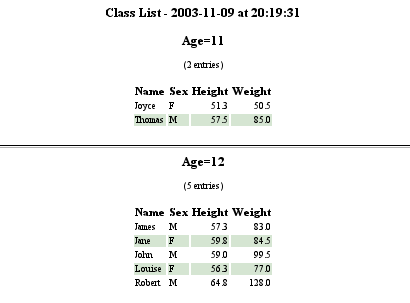
\includegraphics[width=5in]{ages2.png}
\end{goutput}

\subsection{various problems}
\index{Events!table\_head}
\index{Style!table\_head}
The first time this job runs, there is a warning in the log that the table\_head style
was not found.  This is coming from the stripes tagset where the table\_head event
is asking for the table\_head style.  It doesn't really cause any problems but defining
an empty style will take care of the warning.

\begin{sfvcode}
   style table_head
   ;
\end{sfvcode}
 
The other thing that is needed is a style for the number of observations label.  The style has
now grown to look like this.

\begin{fvcode}{datastep_style}{Refined striped style}
    define Style styles.minimal_striped; 
        parent = styles.minimal;

        style header/
            font = (, 4,bold)
        ;

        style Data/
            font = (, 3,normal)
        ;

        style DataStrong from data /
            background=cxD5E5D2
        ;

        style nobs_label from data /
        ;

        style table_head
        ;

        style byline /
           font_size = 5
           font_weight = bold
        ;

        replace Output /
            BorderWidth = 0
            CellSpacing = 1
            CellPadding = 7
            Frame = void
            Rules = none
        ;

    end;
\end{fvcode}


\subsection{Modifying the Byline}
\index{Byline!modification}
All that is left is for the byline to modified to match what the datastep code did.
This part isn't too hard either.  The easiest way to do this is to code it for the
data we are reporting on.  That makes this tagset specific to the task, and not
very reusable.  But it is a good first step.

\index{Variables!Macro}
\index{Events!Nobs\_label}
\index{Events!Byline}
Another option will work nicely to indicate which byline needs to be modified. Luckily
only one by value needs changing.  The end of the byline can be postponed until the 
table ends.  That means that the nobs event from the nobs\_count tagset can handle most 
of the work.  In the interest of versatility the byline and nobs\_label events have
been set up to work together.  If there is no byline, the nobs\_label event handles
the situation by doing the setup that the byline event would have done if there was a byline.

The new tagset and it's output follows.

\begin{fvcode}{by_age_tagset}{Tagset with modified by lines}
    define tagset tagsets.by_age;
        parent=tagsets.nobs_label;
        
        /*-------------------------------------------------------eric-*/
        /*-- Add some extra comments to the doc event.              --*/
        /*----------------------------------------------------8Aug 03-*/
        define event initialize;
            unset $do_nobs;
            do /if $options;

                do /if $options['MODIFY_BY'];
                    eval $modify_by inputn($options['MODIFY_BY'], '7.');
                    do /if missing($modify_by);
                        eval $modify_by 0;
                    done;
                done;

                set $do_nobs "true" /if cmp($options['NOBS_LABEL']), 'yes');

                /*---------------------------------------------------eric-*/
                /*-- From the stripes tagset.                           --*/
                /*------------------------------------------------9Nov 03-*/
                set $alt_row_style $options['ALTERNATE_STYLE']";
            done;

            set $alt_row_style 'DataStrong' /if !$alt_row_style;

        end;    


        /*-------------------------------------------------------eric-*/
        /*-- We want to say two different things depending on the   --*/
        /*-- value in the byline.                                   --*/
        /*----------------------------------------------------7Aug 03-*/
        define event byline;
            /*---------------------------------------------------eric-*/
            /*-- Convert age to a numeric.                          --*/
            /*------------------------------------------------7Aug 03-*/
            eval $byval inputn(scan(value, -1, '='), '7.');
        
            put '<p><div';
            putq ' class=' htmlclass ;
            put ' style="text-align: center;">' nl;

            do /if $byval = $modify_by ;
                put 'The Oldest';
            else;
                put 'Age is ' $byval ;
            done;
            
            /*---------------------------------------------------eric-*/
            /*-- A newline would do, but one way or another we need --*/
            /*-- to flush.  Otherwise the timing goes sour.         --*/
            /*------------------------------------------------8Aug 03-*/
            flush;
            set $byline "true";
        end;
        

        /*-------------------------------------------------------eric-*/
        /*-- The nobs title finishes up the paragraph started with  --*/
        /*-- the byline.                                            --*/
        /*----------------------------------------------------7Aug 03-*/
        define event table_nobs_label;
            style=nobs_label;

            /*---------------------------------------------------eric-*/
            /*-- If we did not get a byline then we want to make    --*/
            /*-- sure the html is still well formed.                --*/
            /*------------------------------------------------8Aug 03-*/
            do /if ^$byline;
                put '<p><div';
                putq ' class="byline"';
                put ' style="text-align: center">' nl;
                unset $byline;
            done;

            put '&nbsp;&nbsp;<span class="' htmlclass '">(' $nobs ' ';

            do /if $nobs = 1; 
                put 'entry)' ;
            else;
                put 'entries)' ;
            done;

            put '</span></div></p>' nl;
        end;

    end;
\end{fvcode}

The proc print that creates this output is still rather simple.  Only the two
macro variables look out of the ordinary.

\begin{sfvcode}
title;

ods tagsets.by_age options(nobs_label='yes' modify_by='16')
    file="ages3.html" (title='Class List')
    style=minimal_striped;

proc sort data=sashelp.class out=myclasssrt;
  by age name sex height weight;
run;

*options obs=6;

proc print data=work.myclasssrt noobs;
    by age;
    pageby age;
run;

ods tagsets.by_age close;
\end{sfvcode}


\begin{goutput}{ages3_out}{Output with modified By lines}
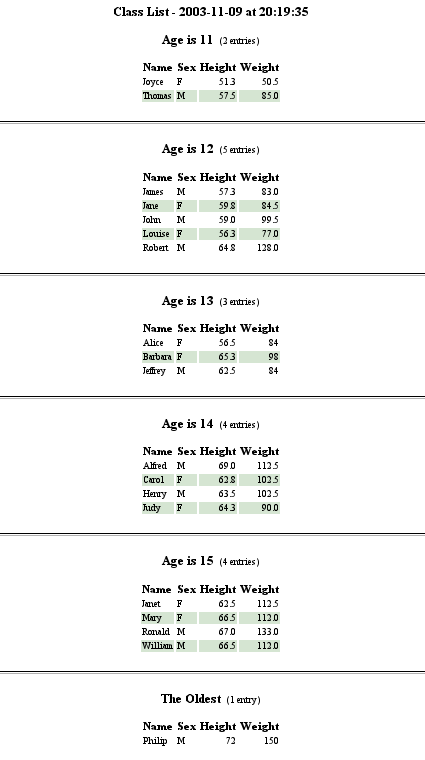
\includegraphics[width=4in]{ages3.png}
\end{goutput}

\subsection{A more flexible solution}
\index{Events!Byline}
\index{Dictionary}
This tagset is simple enough that it doesn't really matter that it's specific to this
data.  But with a little work it can be made more universal.  All it needs is a more
flexible way to indicate which by values need reformatting, and what they should be 
reformatted to.  That can be done with a macro variable. The heart of this tagset
is a dictionary.  When the proc starts the macro variable is parsed and put in 
the dictionary.  The byline event uses the dictionary to decide what to do with
each byline.  

\index{Events!Bygroup}
\subsubsection{More Identify, and Locate}
\index{ByLines}
There is an event called bygroup that surrounds all bygroup processing.  Using the start
of that event to parse the macro variable and set up the by value dictionary for the by lines
that will be coming. All of this requires that the by values are known.  But that
was a prerequesite for this particular problem anyway.

The new mod\_by\_line tagset follows.

\begin{fvcode}{flexible_byline_tagset}{A more versatile byline tagset}
 define tagset tagsets.mod_by_line;
        parent=tagsets.nobs_label;
        
        define event bygroup;
            start:
                /*-----------------------------------------------eric-*/
                /*-- Do not do this if there is no need.            --*/
                /*--------------------------------------------9Nov 03-*/
                break /if ^modify_by;

                break /if cmp($modify_by, modify_by);
                
                unset $byval_subs;
                set $modify_by modify_by;
                
                eval $count 1;
                trigger set_byval_pair;

                do /while !cmp($byval_pair, ' ');

                    set $byval_subs[$byval] $substitution;

                    eval $count $count+1;

                    trigger set_byval_pair;
                done;

        end;

        define event set_byval_pair;     
            set $byval_pair scan($modify_by, $count, '|');
            set $byval scan($byval_pair, 1, ':');
            set $substitution scan($byval_pair, 2, ':');
        end;   
        

        define event byline;
            /*---------------------------------------------------eric-*/
            /*-- Get the by value in string form                    --*/
            /*------------------------------------------------7Aug 03-*/
            eval $byval trim(scan(value, -1, '='));
            
            put '<p><div';
            putq ' class=' htmlclass ;
            put ' style="text-align: center;">' nl;

            do /if $byval_subs[$byval];
                put $byval_subs[$byval];
            else;
                do /if by_label;
                    put by_label $byval;
                else;
                    put value;
                done;
            done;
            
            /*---------------------------------------------------eric-*/
            /*-- A newline would do, but one way or another we need --*/
            /*-- to flush.  Otherwise the timing goes sour.         --*/
            /*------------------------------------------------8Aug 03-*/
            flush;
            set $byline "true";
        end;
        

        define event table_nobs_label;
            style=nobs_label;

            /*---------------------------------------------------eric-*/
            /*-- If we did not get a byline then we want to make    --*/
            /*-- sure the html is still well formed.                --*/
            /*------------------------------------------------8Aug 03-*/
            do /if ^$byline;
                put '<p><div';
                putq ' class=' htmlclass;
                put ' style="text-align: center">' nl;
                unset $byline;
            done;

            put '&nbsp;&nbsp;<span class="' htmlclass '">(' $nobs ' ';

            do /if $nobs = 1; 
                put 'entry)' ;
            else;
                put 'entries)' ;
            done;

            put '</span></div></p>' nl;
        end;

    end;
\end{fvcode}

\index{Debugging}
\index{Putlog}
\index{Statements!Putlog}
\index{Putvars}
\index{Statements!Putvars}
Tagsets like this are not all that difficult except that a mis-spelled variable or
an incorrect if statement will cause it to quietly not do what you asked.  A well placed
putlog or putvars statement can be very revealing.  In this case checking for
the options and memory variables looks like this.

\begin{sfvcode}
   putvars $options _name_ ':' _value_ ':' nl;
   putvars mem _name_ ':' _value_ ':' nl;
   putvars $byval_subs _name_ ':' _value_ ':' nl;
\end{sfvcode}

There are two things in these examples that help with debugging.  The placement
of a character on both sides of a value to reveal whitespace.  The other trick
is to separate the highly visible label from the variable by inserting another
string between them.  Then if the variable does not exist, the label will still
print.

\index{Variables!Macro}
The new job which uses the new macro variables is shown in the following job 
which creates the output in figure \ref{ages4_out} on page \pageref{ages4_out}.

\begin{sfvcode}
title;

ods tagsets.mod_by_line 
    options(nobs_label='yes' 
            by_label='Age is' 
            modify_by='16:The Oldest|11:The Youngest')
    file="ages4.html" (title='Class List')
    style=minimal_striped;

proc sort data=sashelp.class out=myclasssrt;
  by age name sex height weight;
run;

proc print data=work.myclasssrt noobs;
    by age;
    pageby age;
run;

ods tagsets.mod_by_line close;
\end{sfvcode}

\begin{goutput}{ages4_out}{Modifying Bylines, Final output}
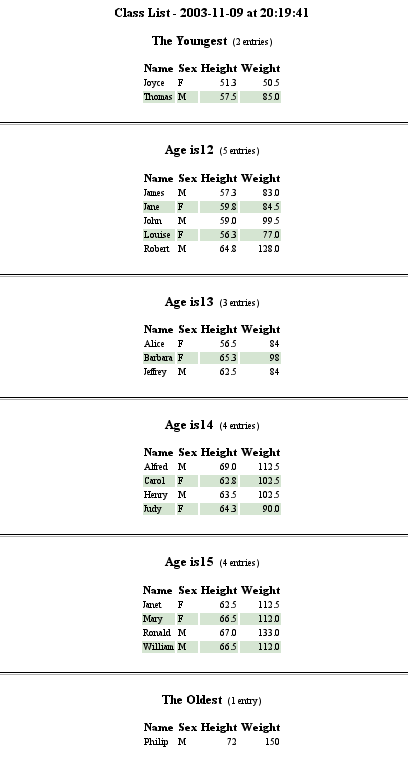
\includegraphics[width=4in]{ages4.png}
\end{goutput}


\section{Summary}
This chapter has shown some of the advantages of converting datastep code
to tagsets.  Tagsets do not pretend to replace datastep, but if responsiblities
are divided between datastep and tagsets then the solution is more open for 
re-use in later solutions.  More power and flexibility is also provided by the
tight integration the output now has with ODS.


%%\cleardoublepage
%%%\chapter{Extended examples}
This chapter will explore some more complex examples.  The
complexity comes mostly from the combination of multiple
techniques.  From a juggler's point
of view, there are just more balls in the air.  But a ball is
still just a ball.  Any given feature of these new tagsets
is still just as simple as it ever was.  This is one of the
wonderful things about tagsets.  It is easy to reuse and 
combine ideas from different tagsets.

\section{Repeating Headers, and Mirrored Row headers}
When tabular output is extremely wide or long it is often hard to tell
what the data is because the haders have scrolled out of view.  This
tagset solves that problem by putting row headers on both sides of the
table.  It also repeats the headers as in our previous example on page
\pageref{repeat3}

\subsection{The Single Stream Solution}
This solution uses a single stream per row to capture all of the row headers.
This works nicely but when a table has multiple row headers the result isn't
as nice as it could be.  Still, this is an important step towards the next
solution.

\subsection{The Multiple Stream Solution}
This solution uses multiple streams to capture the row headers.  Streams
make everything easy.  The easiest thing would be to use one stream to catch
the rowheaders on each row.  But then, the order would be fixed when a row had
multiple column row headers.  It  would be really nice if the row headers would
be reversed when they are printed on the other end of the table.  To do that
each row header will need it's own stream.

\subsection{The Multiple List Solution}
This solution uses lists to capture the row headers text and alignment.
this is a bit more work but makes it easier to manipulate how the row headers
are rendered.

\section{Automatic Panelling}
In this example we will combine our startpage tagset with some a dictionary 
and some new events to create a tagset that automatically panels output.

\subsection{An Extension of Start Page}
sthsnthsn

\subsection{The solution}
tnhsnthsn

\section{HTML forms}
This example uses as simple proc print to create a simple HTML form with 
option menus created by the proc print.  This is a fairly simple example 
that can be extended to use multiple data sets and procedures to create
more complex HTML forms from ODS.

\subsection{Option Lists}

\subsection{Saving the Lists}

\subsection{Creating the Form}

\section{Summary}
These tagsets are another example of how a basic idea can be
extended to create a nicley flexible output destination.  It can be completely
transparent to the user or it's behavior can be modified at will.


\chapter{A feature Rich Tagset}
In this book we have created many tagsets that can each do something special.
The tagsets have been carefully written to enable those features to be
transparent to anyone who uses them.  It is possible that all of these features
be combined into one tagset.  

\section{Which features?}
two - sided, start page, sliders, table head style, stripes, nobs, byline, web site.

\section{Lining up the inheritance}
Some of the existing tagsets con be used just by changing their inheritance.  If the
order of inheretance is chosen with care then the number of changes can be minimized.

\section{Copy and Paste}
It might just be easier to create one big tagset that does it all...

\section{Macro Variables and Tagset Alias}
Turning all of these things on and off presents some special problems.  Each of them
want macro variables, tagset alias or both.

\section{Summary}
Cool.

%%%\cleardoublepage

\part{Usage Notes and Caveat's}
%{
%These chapters cover problems that can be encountered with some
%procedures and the most common uses of the various tagsets that 
%are shipped with SAS.  There are several flavors of HTML that may
%be used for various purposes.  Uploading ODS output to spreadsheets
%is another hot topic.  Several tagsets lend themselves towards that
%goal.  LaTeX is an often overlooked but very versatile family of tagsets.  
%It's usage may be more popular with understanding.  The XML libname
%engine also uses tagsets to define it's output.  Knowing when to
%use the libname engine instead of ODS is an advantage.
%}

%\chapter{Special Cases, Procedures and Operating Systems'}
The examples in this book have shown that there are some problems
when it comes to the Report and Tabulate procedures.  These
problems are surmountable but they do cause some pain.  This
chapter is going to explain the specifics of these problems
and how to work around them.

\section{A Report Procedure problem}
Yet another reason to
convert is that tagsets can be interchanged to create new and 
diffrent outputs.  Usually datastep is used to create HTML, CSV,

\subsection{deferred data}
or DDE to XML,  A different datastep is required for each.  A different
tagset is required for each as well.  The difference is the reusability
and the ease of creation and maintenance.

\section{The Tabulate and Report problem}
More reasons to convert are the availability of style changes, and the
plethora of ODS options that can be used to customize your output.

\subsection{The Table Head section}
sthsthsnt

\subsection{The Table column specifications}
sthsthsnth

\section{HTML on MVS with a PDSE}
When serving web pages that are stored in a PDSE on MVS, the url do not
adhere to the Standards for URI syntax.  Because of this HTML output
that ODS creates will not have links that work.  To fix this there is
a special tagset called MVSHTML that changes the format of the URLS
in the HTML code.  URLS are used in several places, most importantly
in the table of contents, and with the src attribute when including
graphics.  The MVSHTML tagset takes care of all these problems.

\section{Summary}
Through the various examples in this book we have seen the problems
that are caused by the Report and Tabulate procedures.  These problems
are not unsurmountable, but they do complicate the tagsets we create.  
Knowing what the problems are can help save time and frustration when 
creating a tagset.  Or minimize the surprise when a tagset that works 
with other procedures quits working when it comes to using Report or 
Tabulate.



%\cleardoublepage
%%\chapter{Using Tagsets with the Libname XML Engine}
The libname XML Engine also uses tagsets.  all of the output generated
from the XML engine is done through a tagset.  The libname engine's 
tagsets differ somewhat from the tagsets used by ODS Markup.  This chapter
will explain how to use tagsets with the libname engine and how they
differ from those used by ODS.

\section{XML Engine vs. ODS}
ODS is more about reporting and
style.  The XML engine is all about data.  Consequently, the tagsets used by
the Engine are much different from those used by ODS.  The tagsets are not
currently interchangeable (SAS 9.1.3) but that is changing.  The XBRL tagset
works with both ODS and the XML engine.  The XML engine may be able to use 
some of the ODS tagsets with reasonable results.  But ODS usually cannot use 
the engine's tagsets.

The first step towards understanding is to run libname with the short\_map tagset.

\begin{sfvcode}
libname mapxml xml 'map.xml'
tagset=tagsets.short_map;
proc copy in=sashelp out=mapxml;
select class;
run;
\end{sfvcode}

The output from this simple job reveals an event model that is not all that
different from th  ods output.  It's just simpler.

\begin{fvoutput}{Engine_map}{The XML Engine's Event Model}
<?xml version="1.0" encoding="iso-8859-1"?>

<doc operator="eric" sasversion="9.1" 
      saslongversion="9.01.01M0D10062003" 
      date="2003-11-17" time="23:08:50" 
      encoding="iso-8859-1" name="CLASS">
   <doc_head>
   </doc_head>
   <doc_body>
      <proc name="CLASS">
         <table name="CLASS">
            <colspecs name="CLASS">
               <colgroup>
                  <colspec_entry name="Name"/>
                  <colspec_entry name="Sex"/>
                  <colspec_entry name="Age"/>
                  <colspec_entry name="Height"/>
                  <colspec_entry name="Weight"/>
               </colgroup>
            </colspecs>
            <table_head name="CLASS">
               <row name="CLASS">
                  <data>
                  </data>
                  <data>
                  </data>
                  <data>
                  </data>
                  <data>
                  </data>
                  <data>
                  </data>
               </row>
            </table_head>
            <table_body name="CLASS">
               <row name="CLASS">
                  <data name="Name" value="Joyce">
                  </data>
                  <data name="Sex" value="F">
                  </data>
                  <data name="Age" value="11">
                  </data>
                  <data name="Height" value="51.3">
                  </data>
                  <data name="Weight" value="50.5">
                  </data>
               </row>
               <row name="CLASS">
                  <data name="Name" value="Thomas">
                  </data>
                  <data name="Sex" value="M">
                  </data>
                  <data name="Age" value="11">
                  </data>
                  <data name="Height" value="57.5">
                  </data>
                  <data name="Weight" value="85">
                  </data>
               </row>
               <row name="CLASS">
                  <data name="Name" value="Louise">
                  </data>
                  <data name="Sex" value="F">
                  </data>
                  <data name="Age" value="12">
                  </data>
                  <data name="Height" value="56.3">
                  </data>
                  <data name="Weight" value="77">
                  </data>
               </row>
               <row name="CLASS">
                  <data name="Name" value="Jane">
                  </data>
                  <data name="Sex" value="F">
                  </data>
                  <data name="Age" value="12">
                  </data>
                  <data name="Height" value="59.8">
                  </data>
                  <data name="Weight" value="84.5">
                  </data>
               </row>
               <row name="CLASS">
                  <data name="Name" value="James">
                  </data>
                  <data name="Sex" value="M">
                  </data>
                  <data name="Age" value="12">
                  </data>
                  <data name="Height" value="57.3">
                  </data>
                  <data name="Weight" value="83">
                  </data>
               </row>
               <row name="CLASS">
                  <data name="Name" value="John">
                  </data>
                  <data name="Sex" value="M">
                  </data>
                  <data name="Age" value="12">
                  </data>
                  <data name="Height" value="59">
                  </data>
                  <data name="Weight" value="99.5">
                  </data>
               </row>
               <row name="CLASS">
                  <data name="Name" value="Robert">
                  </data>
                  <data name="Sex" value="M">
                  </data>
                  <data name="Age" value="12">
                  </data>
                  <data name="Height" value="64.8">
                  </data>
                  <data name="Weight" value="128">
                  </data>
               </row>
               <row name="CLASS">
                  <data name="Name" value="Alice">
                  </data>
                  <data name="Sex" value="F">
                  </data>
                  <data name="Age" value="13">
                  </data>
                  <data name="Height" value="56.5">
                  </data>
                  <data name="Weight" value="84">
                  </data>
               </row>
</table_body>
</table>
</proc>
</doc_body>
</doc>
\end{verbatim}

Using the event\_map tagset with the same job is even more revealing.  Here is a small
section of that output.

\begin{verbatim}
  <row event_name="row" trigger_name="attr_out" section="body" 
       class="Table" id="CLASS" colcount="5" name="CLASS" 
       index="IDX" just="c">

    <data event_name="data" trigger_name="attr_out" section="body" 
       class="Data" id="CLASS" text="COLUMN" value="Jane" 
       colcount="5" col_id="4" name="Name" type="string" 
       index="IDX" just="0">
    </data>
\end{fvoutput}

\section{Advantages of the XML engine}
It is possible to use ODS tagsets with the libname engine, to a point.  They
don't always work very well.  But the XML Libname engine has several tagsets 
created just for it.  They work better, and they do things that ods doesn't
do all that well.  This is mostly because the datastep's relationship with the
XML engine is much closer than it is with ODS.

\subsection{Control options}
There are also some options that allow control over the form the generated xml
will take.  The increased versatility means that the XML engine can create just
about any XML format that you can imagine.

\section{The Tagsets}
The XML engine's tagsets are designed around a single abstract tagset that should
never be used directly, It won't produce much in the way of output if you do.
The design allows most of the tagsets to be very simple.  But understanding it
all is a bit more complicated.

\section{Summary}
When it comes to importing SAS output into spreadsheets there are many choices.
None of them work perfectly.  But some of them work very well.  DDE has been a
popular choice, but using it is somewhat painful.  The excelXP tagset is probably
a better choice for most uses.  The msOffice2K and phtml tagsets also work very well.



%%\cleardoublepage

% -----------------------document end
\backmatter
\part{Appendices}
\appendix
\begin{appendix}
\chapter{Quick Reference Guide}
\section{Useful tagsets}

\begin{description}

\tagsetitem{HTML4}{HTML, HTML4}

Generates W3C compliant HTML4.

\tagsetitem{PHTML}{pHTML}

HTML with a simplified Stylesheet.

\tagsetitem{HTMLCSS}{HTMLcss}

HTML 4.0 with a complete stylesheet definition.
Only slightly different HTML from the HTML4 tagset.

\stagsetitem{XHTML}

This is an XHTML destination that is almost identical
to HTML4.

\tagsetitem{CSV}{CSV}

CSV that contains only tabular data.

\tagsetitem{CSVALL}{CSVall}

CSV with titles, footnotes, notes, and bylines.

\stagsetitem{CSVbyline}

CSV with tables and bylines.

\stagsetitem{RTF}

This is an RTF destination with both vertical and horizontal 
measurement among other things.  The RTF tagset is the future
of ODS RTF.

\tagsetitem{LaTeX}{Latex}

The basic LateX destination for creating complete LaTeX documents.

\stagsetitem{ColorLaTeX}

The basic LateX destination with the color package added.

\stagsetitem{SimpleLaTeX}

A simple LateX destination without SAS specific LaTeX macros.

\stagsetitem{TablesOnlyLaTeX}

A very simple LateX destination that only generates tables.
This is perfect for use with newfile=output to create files
with individual tables for inclusion in other LaTeX documents.

\tagsetitem{Troff}{Troff}

This is a basic troff tagset that is useful for creating black and
white typeset documents, in pdf and postscript.  Troff is used to
typeset the man pages on Unix systems.

\tagsetitem{MSOffice2k}{MSOffice2k}

An HTML tagset with Microsoft specific XML embedded for better
loading into Microsoft Office products.

\tagsetitem{cHTML}{cHTML}

Compact HTML creates very compact HTML with no style. 
Used primarily for PDA's and phones.

\tagsetitem{Imode}{Imode}

Imode is a subset of HTML that has no tabular support.
Used for PDA's and phones in Japan and some other countries.

\tagsetitem{WML}{WML}

Wireless markup language is a small footprint XML for
PDA's and phones.

\tagsetitem{WMLolist}{WMLolist}

Wireless markup tagset that creates a table of contents as
an option list.

\tagsetitem{Default}{XML}

An XML definition that is closely modeled after the internals of
ODS.

\stagsetitem{Event\_map}

Event map creates an XML file that shows all events as XML tags.
Event map prints a large number of attributes as part of it's output.

\stagsetitem{Short\_map}

Short map is a much less verbose mapping tagset that can be much easier
to read.  This is handy for showing the event model when looking for
events, names, labels and values.

\stagsetitem{Super\_map}

Super map is a mapping tagset that can be controlled through options.
It can be verbose, or not.  Among other things it can look for 
specific values within the event model and show only events that match.


\stagsetitem{Style\_Popup}

Style popup is a child of HTML4 it creates HTML with a popup window that displays
ODS style information for all the HTML elements on the page.

\stagsetitem{Style\_Display}

Style Display is a child of Style Popup that creates a sample page that contains
examples of all of the different style elements that ODS regularly defines.

\stagsetitem{OdsStyle}

The Ods style tagset writes a proc template program to the stylesheet file.
The program generated is a style template with no inheritance that makes it
easier to see all the attributes in use for any given element.  It is not a
good way to keep a style template because of maintainence issues.

\tagsetitem{Pyx}{Pyx}

Pyx is a very simple markup language that lists every single item on a separate
line.  Pyx is very easy to parse, grep and mold into other shapes including XML.


 


\end{description}

\section{Tagset attributes}

\begin{description}

\commanditem{Map}{string}

Map is a list of special characters that need to be
translated in order to work with the target markup language.
A typical value for HTML or XML might be "\&<>'"

\commanditem{MapSub}{string}
Mapsub is a list of strings that will replace the characters
listed in the map.  The strings separater is the first character
in the list.  A typical value for HTML is "/\&amp;/\&lt;/\&gt;/\&apos;/".

\commanditem{Split}{string}

The value of slit is what the tagset will use in place of split characters
when they are encountered.  The typical value for HTML is "<Br>".

\commanditem{NoBreakSpace}{string}

The value of NoBreakSpace is what the tagset will use for non-breaking spaces.
The default is a regular space.  HTML generally uses "\&nbsp;".

\commanditem{Default\_Event}{string}

This the name of an event to use when the ODS requested event is not defined
within the tagset.

\commanditem{Output\_Type}{string}

Output type is the type of output being created.  HTML, LaTeX, XML, CSV, etc.
This is primarily used by the SAS results window so that it can display the
output correctly.

\commanditem{Log\_Note}{string}

Log Note is a note that will be printed to the log every time the tagset is used.
Usage notes, release date and revision number are good things to put in the lognote.

\commanditem{Trademark}{string}

Trademark is the string to use in place of the SAS control code for trademark.
HTML uses '\&trad;'.

\commanditem{Registered\_TM}{string}

Registered\_TM is the string to use in place of the SAS control code for registered trademark.
HTML uses '\&reg;'.

\commanditem{Copyright}{string}

Copyright is the string to use in place of the SAS control code for copyright.
HTML uses '\&copy;'.

\commanditem{Image\_Formats}{string}

Image formats is a space delimited list of image formats supported by the target output
type.  Valid values are png, gif, jpeg, bmp, svg, java, activex, ps, psepsf, epsi.
If the image device is not set to a valid image format, then the first image format
in the list will be used to create the image.

\commanditem{BeginWellFormed}{string}
\commanditem{EndWellFormed}{string}

BeginWellFormed is a string that indicates what well formed markup for the target
output begins with.  All text will be checked to see if it begins and ends with
the value of beginwellformed and ends with the value of endwellformed, excluding
leading and trailing whitespace.  If the string is matched, then the characters
in the string will not be remapped by the values of map and mapsub.


\commanditem{Default\_style}{string}

Default style is the name of the default style to use when a style is not
specified on the ods statement.

\commanditem{Body}{string}

Body is the name to use for the body file when automatic packages are in use.
When an automatic package is in use, the file name given on the ods statement
becomes the package archive name.  The body name given here becomes the body
file actually created and placed within the archive.

\commanditem{Contents}{string}

Contents is the name to use for the contents file when automatic packages are in use.

\commanditem{Pages}{string}

Pages is the name to use for the pages file when automatic packages are in use.

\commanditem{Frame}{string}

Frame is the name to use for the frame file when automatic packages are in use.

\commanditem{Stylesheet}{string}

Stylesheet is the name to use for the stylesheet file when automatic packages are in use.

\commanditem{Code}{string}

Code is the name to use for the code file when automatic packages are in use.

\commanditem{Data}{string}

Data is the name to use for the data file when automatic packages are in use.


\commanditem{Body\_Mimetype}{string}

Body\_Mimetype is the mimetype to use for all body files created.

\commanditem{Contents\_Mimetype}{string}

Contents\_Mimetype is the mimetype to use for all contents files created.

\commanditem{Pages\_Mimetype}{string}

Pages\_Mimetype is the mimetype to use for all pages files created.

\commanditem{Frame\_Mimetype}{string}

frame\_Mimetype is the mimetype to use for all frame files created.

\commanditem{Stylesheet\_Mimetype}{string}

Stylesheet\_Mimetype is the mimetype to use for all stylesheet files created.

\commanditem{Code\_Mimetype}{string}

Code\_Mimetype is the mimetype to use for all code files created.

\commanditem{Data\_Mimetype}{string}

Data\_Mimetype is the mimetype to use for all data files created.

\commanditem{Default\_Mimetype}{string}

Default\_Mimetype is the mimetype to use for all files that do not specify a mimetype.

\commanditem{Indent}{Integer}

The value of indent is used to determine how many spaces the Ndent and Xdent statements
move the indention level.

\commanditem{Breaktext\_Width}{Integer}

Breaktext\_width is the maximum {\bfseries width of space} that will
be considered for placement of automatic breaks in text.  If the width
of the space is greater than this value the text will not be broken.

\commanditem{Breaktext\_Length}{Integer}

Breaktext\_length is the maximum {\bfseries length of text} which will be considered for placement 
of automatic breaks.  If the text is longer than this value then no breaks will be inserted
automatically

\commanditem{Breaktext\_Ratio}{Number}

Breaktext\_Ratio is the ratio of the width of space to the length of the text which is supposed to fit in it.  Like the other two attributes, this attribute serves to narrow the the string and
width combinations that will be considered for splitting.  The text length and width must fall
within this ratio before they will be considered for forced splits.


\commanditem{Upi}{Integer}
\commanditem{Fontpad}{Integer}

\commanditem{Parent}{Tagset Name}

Parent is the name of a tagset to inherit events and attribute settings from.

\commanditem{Package}{Package Template Name}

Package template name.  This turns on automatic packages for the tagset.
When set, the file specified on the ods statement becomes the package archive
name. All output from the destination will be placed in that archive.  The
actual files created will depend upon the settings of the package file attributes,
body, contents, pages, frame, stylesheet, code and data.

\commanditem{Stacked\_columns}{yes | no | on | off}

When set to off, stacked column events will not be sent to the tagset.  Except for
the Freq Procedure with cross tabular reports.

\commanditem{Embedded\_stylesheet}{yes | no | on | off}

If set to on, stylesheet events will be sent to the body file when no stylesheet
file is specified on the ods statement.

\commanditem{Pure\_style}{yes | no | on | off}

Normally, all style information is surfaced in the stylesheet events and is filtered
in subsequent events.  Setting pure\_style to yes will cause all events to receive all
the style information all of the time.

\commanditem{Measurement}{yes | no | on | off}

Turn contents measurement on.  When on, the output is measured vertically and
horizontally and ajusted to fit on the page.  Primarily used by the RTF, LaTeX
and any other markup that needs page formatting.

\commanditem{Ext\_Graph\_Instance}{yes | no | on | off}
\commanditem{No\_Byte\_Order\_Mark}{yes | no | on | off}

If set No Byte order mark will be generated for XML files.

\commanditem{Hierarchical\_Data}{yes | no | on | off}

When hierarchical data is set to yes, The Tabulate and Freq procedures
generate events in a tree view rather than a tabular view.

\commanditem{Uniform}{yes | no | on | off}

\commanditem{Reference\_Image}{yes | no | on | off}

\end{description}

\section{Event attributes}

\begin{description}
\commanditem{STYLE}{Style Element Name}

This is the name of the style element that the event should use.

\commanditem{Pure\_Style}{yes | no | on | off}

When pure style is set to yes, all style attributes will be available, they will not
be filtered as if they were already defined in a stylesheet.

\commanditem{File}{(frame | contents | style | code | body | default | pages | data )}

The file attribute determines which output file the event will write it's output to.
If the file was not specified on the ods statement, the event will generate no output.

\end{description}

\section{Event Statements}
\begin{description}

%\item[\commandnames{Block}]  \commandargs{event-name <condition>}
\commanditem{Block}{event-name <condition>}

Blocks the use of the specified event.  Use the unblock command to
make the event usable again.

\commanditem{Break}{<condition>}

Break stops an event from continuing. The event is exited immediately, no statements below
the break statement will be executed.

\commanditem{Continue}{<condition>};

When placed within an if or while, execution goes back to the top for re-evaluation.

\commanditem{Close}{<condition>};

Close stops the flow of output to the current stream. 
Output is redirected to the current output file.

\commanditem{Delstream}{(stream-name | variable) <condition>};

Completely deletes the specified stream.  This is different from an unset which
simply clears the contents of the stream.

\commanditem{Do}{<condition>}

Starts a statement block. 

\commanditem{Done}{}

Ends a statement block. 

\commanditem{Else}{<condition>};

Begins a statement block that executes if the Do it belongs to is false. This is more efficient and easier to read than the common alternative of two lines with one if negated. In the case of a Do /while the else only executes if the while is false on the first evaluation. Multiple elses may be chained by using an if.

\commanditem{Eval}{variable-name>[(<number>|<key>)]<where-clause>};

Eval sets the value of the variable to the return value of the where clause. The variable's type can be numeric or string depending upon the where clause. The standard SAS Language where processing syntax applies. 

\commanditem{Flush}{<condition>};

Forces any buffered output to be written to the current output file or stream.

\commanditem{Iterate}{variable-name <condition>};

Creates or initializes an iterator for the given list or dictionary variable. The first value of the variable will be placed into \_value\_. If it is a dictionary the key will be placed in \_name\_.

\commanditem{Ndent}{<condition>};

Indents output one indentation level using the number of spaces specified by the INDENT= attribute. 

\commanditem{Next}{variable-name <condition>};

Causes the variables iterator to increment to the next value and repopulate the variables \_value\_ and \_name\_ as appropriate.

\commanditem{Open}{(stream-name | variable) <condition>};

Opens the specified stream. If the stream does not exist it is created. If a variable is given, the value of that variable becomes the stream name.  If a different stream is open, that stream is closed. All PUT statements that occur after the open are appended to the stream and not to the output file.

\commanditem{PUT | PUTL | PUTQ}{(<variable> <String> <function> <nl|cr|lf> )* <conditon>};

Writes text or variable data to an output file. In general, the syntax consists of a space-delimited list of strings, variables, new line, or data step functions, followed by an optional condition. Functions may not be nested. A string preceding a variable creates a string-value pair, Both the label string and the variable will print as long as the variable has a value.
PUT is the basic statement in its simplest form. For example:
    put 'Beginning of output.';
PUTL adds a new line to the end of the output. This is useful when an event's output is large.
PUTQ places quotes around the value in a variable. For example, the PUTQ statement
    putq "color=" foreground;
results in the following output: 

color="blue"
To write a new line, use any of these new line arguments: CR, NL, or LF. All three work the same.
PUT statements pair strings with variables. If a string is followed by a variable, they become a pair. If the variable has a value, then the pair becomes output. If not, then neither will be output. For example, for the following PUTQ statement, if none of the variables have a value, the output would be <table>:
    putq "<table" " background" background "
    foreground=" foreground "cellpadding=" cellpadding ">" nl;

\commanditem{Putlog}{(<variable> <String> <function> )* <conditon>};

Putlog works just like put except that the output is directed to the log. 
Putlog does not accept newlines.

\commanditem{Putstream}{(stream-name | variable) <condition>};

Writes the contents of the specified stream to the current output file. 

\commanditem{Putvars}{(variable-group | list | dictionary) (<variable> <String> <function> <nl|cr|lf> )* <conditon>};

Putvars is like the put statement except that it loops through all of the variables in the variable group. Each iteration populates special variables that can be used in the format. \_name\_ holds the name of the variable. \_value\_ holds the value of the variable.  This is very similar to a simple loop using iterate and next.  All in one statement.

Values for variable-group are
EVENT
STYLE
DYNAMIC
MEMORY
STREAM

    putvars event   \_name\_ ':' \_value\_ nl;

\commanditem{Set} {variable-name <[(<number>|< key>)]> (<variable> <String> <function>)* <conditon>};

Sets the specified variable with the value of any strings, variables, or data step functions, following the variable name. Functions may not be nested. The variable name must be a memory or stream variable or stream variable, that is, preceded by a single or double dollar sign (\$ or \$\$). The arguments follow the same behavior and syntax as the PUT statement. SET does not accept newlines. The only limitation is that a user variable cannot be set to a stream variable. Variables can be set to themselves. It should be noted that setting a stream to itself can be inefficient and slow. 

\commanditem{Stop}{<condition>};

Causes execution to jump to the end of the current statement block. 

\commanditem{Trigger}{event-name <START | FINISH> <condition>};

Executes another event inline. If you are in the start section of an event, then any event triggered also runs its start section. If you are in the finish section, then the triggered event runs its finish. If a triggered event does not have start or finish sections, then it runs the statements it does have. A trigger can also explicitly ask for an event's specific section.


\commanditem{Unblock}{event-name <condition>};

Re-enables a previously blocked event. To disable an event, use the BLOCK statement. 

\commanditem{Unset}{(ALL | variable-name [(<number>|< key>)]) <condition>};

Remove, delete, clear, the variable given.

\commanditem{Xdent}{<condition>};

Removes one indention level from the output.

\end{description}

\section{If Statements}

All of these items are conditons that can be used anywhere you see
<condition> in the reference.  Conditions are separated from the statement
with a /.  if, when, and where can be used as desired for readability. 
While and breakif both give special behavior to the statements they are
connected to.  The test can can be any of the 5 builtin tests or it can
be a where clause.  The 5 builtin functions are Any, cmp, contains, exists,
or a variable alone. 

\large{Statement}\large\textbf{/ (<if | when | where | while | breakif>) } \large\textsc{any | cmp | contains | exist | variable | where clause}

\begin{description}
\commanditem{Any}{(variable, <variable>*)}

checks a list of variables for values. If any of the variables has a value, then the condition is true and the statement executes.

\commanditem{BreakIf}{<condition>}

When true break if executes the current line and then breaks out of the event. 

\commanditem{Cmp}{(variable | string, variable | string)}

compares a string to a variable or a list of variables for equality. Cmp is case insensitive. For example:

\commanditem{Contains}{(variable | string, <variable | string >)};

looks inside the first string for the second string.  Case sensitive.

\commanditem{EXIST | EXISTS}{(variable, <variable>*)}

checks a variable or a list of variables to determine if a value exists for each. If all of the variables have a value, then the condition is true and the statement executes. If a variable has an empty string of length 0, then the value does not exist and the statement does not execute. 

\commanditem{Variable}{}

An if that consists of a single variable will be evaluated according to its type. If it is a string variable the test will be for length. If it is a numeric variable the test will be for the value. If the variable is a dictionary element ("\$dict[\$key]") the the result is true if the key is defined, otherwise false." 

\commanditem{While}{<condition>}

While is only valid on a Do statement. It indicates that the corresponding statement block should loop until the while becomes false.

\end{description}

\chapter{Variables}
\section{Event Variables}
\subsection{508 Accessibility}

All of these variables for 508 Accessiblity can be set in the table template.

\begin{description}
\variable{508 Accessibility}{Abbr}
 Abbreviation; useful for compliance with Section 508 of the U.S. Rehabilitation Act of 1973.

\variable{508 Accessibility}{Acronym}
Acronym

\variable{508 Accessibility}{Alt} 
Alternate description.

\variable{508 Accessibility}{Caption} 
	Captions for tables.
\variable{508 Accessibility}{LongDesc} 
	Long table description.
\variable{508 Accessibility}{Summary} 
        Table Summary.

\end{description}

\subsection{Data}

\begin{description}
\variable{Data}{\_Name\_} 
    Name of the current variable or key. Used by putvars, iterate and next

\variable{Data}{\_Value\_} 
    Value of the current variable or variable element. Used by putvars, iterate and next

\variable{Data}{Dname} 
    Name of the column in the data component to associate with the current column. Set with the DATANAME= attribute in the column definition.

\variable{Data}{Label} 
    Label for the variable. Set with the LABEL= attribute in the column definition.

\variable{Data}{Name} 
    Name of the variable. Set with the VARNAME= attribute in the column definition.

\variable{Data}{Value} 
    Current value. data, header, title, byline, note, etc.

\end{description}

\subsection{Data Formatting}
\begin{description}

\variable{Data Formatting}{Closure} 
    Describes whether the endpoints of a format range are included or excluded, i.e. <-, -, -<, <-<, etc.


\variable{Data Formatting}{DataEncoding} 
Encoding type for Raw value, always Base64.

\variable{Data Formatting}{DataType} 
Picture format option.

\variable{Data Formatting}{DefWidth} 
Format Default Width

\variable{Data Formatting}{Fill} 
Picture format option.

\variable{Data Formatting}{FMTLang} 
Picture format option.

\variable{Data Formatting}{Fuzz} 
Format option.

\variable{Data Formatting}{Max} 
Format option

\variable{Data Formatting}{Min} 
Format option

\variable{Data Formatting}{Missing} 
Value that indicates that no data value is stored. By default, SAS uses a single period (.) for a missing numeric value and a blank space for a missing character value. In addition, for a numeric missing value, a special missing value can be used to represent different categories of missing data by assigning the letters A - Z or an underscore.

\variable{Data Formatting}{MultiLabel} 
Format option.

\variable{Data Formatting}{Multiplier} 
Picture format option.

\variable{Data Formatting}{NoEdit} 
Picture format option

\variable{Data Formatting}{No\_Wrap} 
Places a NOWRAP attribute in the tag, so that the browser doesn't insert a line break. NOWRAP is automatically added to a <TD> in HTML. This is important, for example, if the cell contents are math, because the browser might otherwise break a line after a negative sign.

\variable{Data Formatting}{NotSorted} 
Format option

\variable{Data Formatting}{Precision} 
Number of places to the right of the decimal.

\variable{Data Formatting}{Prefix} 
Picture format option.

\variable{Data Formatting}{RangeEnd} 
End value of a range in a format.

\variable{Data Formatting}{RangeStart} 
Start value of a range in a format

\variable{Data Formatting}{Round} 
Format option

\variable{Data Formatting}{Base64} 
encoding of the stored machine representation of the original value.

\variable{Data Formatting}{SASFormat} 
SAS format used to format the value.

\variable{Data Formatting}{Scale} 
Total number of places in the floating point number.

\variable{Data Formatting}{Type} 
Type of data, which can be STRING, DOUBLE, CHAR, BOOL, or INT.

\variable{Data Formatting}{UnformattedType} 
Data type before formatting.

\variable{Data Formatting}{UnformattedValue} 
Value before formatting.

\variable{Data Formatting}{UnformmatedWidth} 
Width before formatting.

\end{description}

\subsection{Event MetaData}


\begin{description}

\variable{Event Metadata}{Empty} 
Flag to determine whether event is called as an empty tag.

\variable{Event Metadata}{Event\_Name} 
SAS Requested event name.

\variable{Event Metadata}{State} 
Current state of the event, which is either START or FINISH.

\variable{Event Metadata}{Trigger\_Name} 
Name of the current event if in a triggered event

\end{description}

\subsection{Graph}

\begin{description}

\variable{Graph}{Archive} 
Points to the location of the jar files. Used by SAS/GRAPH.

\variable{Graph}{ClassId} 
Identifier used by MS Windows to instantiate active controls.

\variable{Graph}{Coordinate} 
Coordinate in a map area. Used by SAS/GRAPH.

\variable{Graph}{Grseg} 
The current graph image is a Grseg.

\variable{Graph}{Image\_Formats} 
Specifies a comma-separated string of image types. The image types are the same as what SAS/GRAPH can produce, for example, GIF, JPG, PNG.

\variable{Graph}{Shape} 
Shape of the clickable map. Used by SAS/GRAPH.


\end{description}

\subsection{Measured}

\begin{description}

\variable{Measured}{Blue} 
\variable{Measured}{Bottom} 
\variable{Measured}{Green} 
\variable{Measured}{KeepN} 
\variable{Measured}{Left} 
\variable{Measured}{List\_Index} 
\variable{Measured}{NOCenter} 
\variable{Measured}{Page\_Columns} 
\variable{Measured}{SectionData} 
\variable{Measured}{Red} 
\variable{Measured}{Right} 
\variable{Measured}{Top} 
\variable{Measured}{Vmerge} 


\end{description}

\subsection{Miscellaneous}

\begin{description}

\variable{Miscellaneous}{Anchor} 
Current anchor, which is the last value of the anchor tag. For example, IDX.

\variable{Miscellaneous}{Data\_Viewer} 
Name of the Data Viewer, Table, Batch, Tree, Graph, Report, Print, etc

\variable{Miscellaneous}{Date} 
The Date Formatted as YYYY-MM-DD.

\variable{Miscellaneous}{Dest\_File} 
Current destination file. Values include BODY, CONTENTS, PAGES, FRAME, CODE, STYLESHEET, DATA.

\variable{Miscellaneous}{FirstPage} 
Specifies that the current page is the first page of the output file.

\variable{Miscellaneous}{Language} 
Language of the current output. Currently, only set when it is an Asian language.

\variable{Miscellaneous}{Output\_Label} 
Label of the current output object.

\variable{Miscellaneous}{Output\_Name} 
Name of the current output object.

\variable{Miscellaneous}{Output\_Type} 
Output type as specified in the tagset.

\variable{Miscellaneous}{Page\_Count} 
Page count since the files were opened.

\variable{Miscellaneous}{Proc\_Count} 
How many procedures have run since the files were opened.

\variable{Miscellaneous}{Proc\_Name} 
Name of the current procedure.

\variable{Miscellaneous}{SASLongVersion} 
Long format of the SAS version.

\variable{Miscellaneous}{SASVersion} 
Short format of the SAS version.

\variable{Miscellaneous}{Space} 
String that the tagset uses for a nonbreaking space.

\variable{Miscellaneous}{Split} 
String that the tagset uses for line breaks.

\variable{Miscellaneous}{Style} 
Current style in use.

\variable{Miscellaneous}{Style\_Element} 
Name of the current style element, Always populated when possible. Where htmlclass is only populated when using stylesheets.

\variable{Miscellaneous}{Suppress\_Charset} 
The Suppress Charset Registry setting.

\variable{Miscellaneous}{Time} 
The time formatted as HH:MM:SS.

\variable{Miscellaneous}{TOCLevel} 
Table of contents level.

\variable{Miscellaneous}{Total\_Page\_Count} 
Page count since the ODA was opened.

\variable{Miscellaneous}{Total\_Proc\_Count} 
How many procedures have run since the ODA opened.

\end{description}

\subsection{ODS Statement}

\begin{description}

\variable{ODS Statement}{Author} 
Author of the output. Specified from the ODS statement or is the user that is running SAS.

\variable{ODS Statement}{BaseName} 
BASE= option as set in the ODS statement.

\variable{ODS Statement}{Body\_Name} 
Name of the body file.

\variable{ODS Statement}{Body\_Title} 
Title of body file.

\variable{ODS Statement}{Body\_URL} 
URL of the body file.

\variable{ODS Statement}{Code} 
Used by SAS/GRAPH.

\variable{ODS Statement}{CodeBase} 
The codebase used by SAS/GRAPH.

\variable{ODS Statement}{Code\_Name} 
Name of the code file.

\variable{ODS Statement}{Code\_Title} 
Title of code file.

\variable{ODS Statement}{Code\_URL} 
URL of the code file.

\variable{ODS Statement}{Contents\_Name} 
Name of the contents file.

\variable{ODS Statement}{Contents\_Title} 
Title of contents file.

\variable{ODS Statement}{Contents\_URL} 
URL of the contents file.

\variable{ODS Statement}{Data\_Name} 
Name of the data file.

\variable{ODS Statement}{Data\_Title} 
Title of data file.

\variable{ODS Statement}{Data\_URL} 
URL of the data file.

\variable{ODS Statement}{Encoding} 
The real world encoding which corresponds to the encoding specified. ex. utf8, iso-8859-1.

\variable{ODS Statement}{Frame\_Name} 
Name of the frame file.

\variable{ODS Statement}{Frame\_Title} 
Title of frame file.

\variable{ODS Statement}{Frame\_URL} 
URL of the frame file.

\variable{ODS Statement}{Graph\_Path\_Name} 
The graph path as given on the ODS statement

\variable{ODS Statement}{Graph\_Path\_URL} 
The graph path URL.

\variable{ODS Statement}{No\_Bottom} 
Non-zero if the No\_Bottom\_Matter option was specified.

\variable{ODS Statement}{No\_Top} 
Non-zero if No\_Top\_Matter option option was specified

\variable{ODS Statement}{Operator} 
Operator. Set from the ODS statement or is the user that is running SAS.

\variable{ODS Statement}{Pages\_Name} 
Name of the pages file.

\variable{ODS Statement}{Pages\_Title} 
Title of pages file.

\variable{ODS Statement}{Pages\_URL} 
URL of the pages file.

\variable{ODS Statement}{Path} 
Path as set by the ODS statement.

\variable{ODS Statement}{Path\_Name} 
The Path as given on the ODS statement.

\variable{ODS Statement}{Path\_URL} 
The path URL.

\variable{ODS Statement}{Stylesheet\_Name} 
Name of the stylesheet file.

\variable{ODS Statement}{Stylesheet\_Title} 
Title of stylesheet file.

\variable{ODS Statement}{Stylesheet\_URL} 
URL of the stylesheet file.

\variable{ODS Statement}{Tagset} 
Name of the current tagset.

\variable{ODS Statement}{Tagset\_Alias} 
Tagset alias, as given by the alias attribute on the ODS statement.

\variable{ODS Statement}{Title} 
Title from the ODS statement.

\variable{ODS Statement}{TranTab} 
Translation table name for character conversions.

\end{description}

\subsection{Table}

\begin{description}

\variable{Table}{CLabel} 
Label for the output object in the contents file, the Results window, and the trace record. Set with the CONTENTS\_LABEL= attribute in the table definition.

\variable{Table}{Colcount} 
Number of columns in the current table.

\variable{Table}{Colend} 
Ending column number.

\variable{Table}{Colspan} 
Number of columns that the cell spans.

\variable{Table}{Colstart} 
Column number for which the cell starts.

\variable{Table}{Data\_Row} 
Specifies that the current row is a data row.

\variable{Table}{First\_Stacked\_Value} 
Specifies that this is the first value in a set of stacked values.

\variable{Table}{Last\_Stacked\_Value} 
Specifies that this is the last value in a set of stacked values.

\variable{Table}{Is\_Stacked} 
TRUE if the Current column is a stacked column.

\variable{Table}{Row} 
Current table row, which includes headers.

\variable{Table}{RowSpan} 
Number of rows that the current cell spans.

\variable{Table}{Section} 
Section of the table, which can be HEAD, BODY, or FOOT.

\variable{Table}{Width} 
Width. Most commonly used for COLSPECS.

\end{description}

\subsection{Title and Note Formatting}

\begin{description}

\variable{Title and Note Formatting}{After} 
AFTER	 Specifies that the current note is an after note (see the documentation for the NOTES statement and the NOTES= option).

\variable{Title and Note Formatting}{Before} 
Specifies that the current note is a before note (see the documentation for the NOTES statement and the NOTES= option).

\variable{Title and Note Formatting}{Hidden} 
Specifies when the current object is hidden. Generally used when creating the table of contents.

\variable{Title and Note Formatting}{In\_Association} 
Specifies inside an association.

\variable{Title and Note Formatting}{In\_Caption} 
Specifies inside the caption part of an association.

\variable{Title and Note Formatting}{Is\_Note} 
Specifies that the current procedure title is a note.

\variable{Title and Note Formatting}{Is\_Title} 
Specifies that the current procedure title is a title.

\end{description}

\subsection{URL}

\begin{description}

\variable{URL}{NoBase} 
NOBASE	Flag to determine whether to use the value for BASE= as part of the URL. 0 uses BASE=. 1 does not use BASE=.

\variable{URL}{Target} 
TARGET	Target that is associated with the URL.

\variable{URL}{URL} 
Fully formed URL.

\end{description}

\subsection{XML Libname Engine}

\begin{description}

\variable{XML Libname Engine}{ID} 
\variable{XML Libname Engine}{SUFFIX} 

\variable{XML Libname Engine}{XMLDataForm} 
Specifies whether the tag for an element to contain SAS variable information (name and data) is to appear in open element or enclosed attribute format. Used by the XML LIBNAME engine.

\variable{XML Libname Engine}{XMLMetaData} 
Specifies whether to generate schema-related information.

\variable{XML Libname Engine}{XMLSchema} 
Specifies whether to generate schema-related information.

\variable{XML Libname Engine}{tag\_Name} 
Specifies a dynamic tagname defined by the data.

\variable{XML Libname Engine}{XMLCONTROL} 
\variable{XML Libname Engine}{XMLCDATA} 
\variable{XML Libname Engine}{XMLPARM} 

\end{description}

\section{Style Variables}
\subsection{Borders}

\begin{description}

\variable{Borders}{BorderBottomColor} 
Border Color

\variable{Borders}{BorderBottomStyle} 
Border Style: Dotted, Dashed, Solid, Double, Groove, Ridge, Inset, Outset, Hidden.

\variable{Borders}{BorderBottomWidth} 
Border Width

\variable{Borders}{BorderColor} 
Color of the border if the border is just one color.

\variable{Borders}{BorderColorDark} 
Darker color in a border that uses two colors to create a three-dimensional effect.

\variable{Borders}{BorderColorLight} 
Lighter color in a border that uses two colors to create a three-dimensional effect.

\variable{Borders}{BorderLeftColor} 
Border Color

\variable{Borders}{BorderLeftStyle} 
Border Style: Dotted, Dashed, Solid, Double, Groove, Ridge, Inset, Outset, Hidden.

\variable{Borders}{BorderLeftWidth} 
Border Width

\variable{Borders}{BorderRightColor} 
Border Color

\variable{Borders}{BorderRightStyle} 
Border Style: Dotted, Dashed, Solid, Double, Groove, Ridge, Inset, Outset, Hidden.

\variable{Borders}{BorderRightWidth} 
Border Width

\variable{Borders}{BorderRightStyle} 
Border Style: Dotted, Dashed, Solid, Double, Groove, Ridge, Inset, Outset, Hidden.

\variable{Borders}{BorderTopColor} 
Border Color

\variable{Borders}{BorderTopStyle} 
Border Style: Dotted, Dashed, Solid, Double, Groove, Ridge, Inset, Outset, Hidden.

\variable{Borders}{BorderTopWidth} 
Border Width

\variable{Borders}{BorderWidth} 
Width of the border of the table.

\end{description}

\subsection{Font}

\begin{description}

\variable{Borders}{color} 
Color of the text.

\variable{Borders}{FontFamily} 
Font family.

\variable{Borders}{FontSize} 
Size of the font.

\variable{Borders}{FontStyle} 
Style of the font.

\variable{Borders}{FontWeight} 
Font weight.

\variable{Borders}{FontWidth} 
Font width.

\variable{Miscellaneous}{textdecoration} 
\variable{Miscellaneous}{textindent} 

\end{description}

\subsection{Background}

\begin{description}

\variable{Background}{BackgroundColor} 
Color of the background.

\variable{Background}{BackgroundImage} 
Background image.

\variable{Borders}{Watermark} 
Specifies whether to make the image that is specified by BACKGROUNDIMAGE into a watermark.

\variable{Background}{BackgroundRepeat} 

\variable{Background}{backgroundPosition} 

\end{description}

\subsection{Frame}

\begin{description}

\variable{Frame}{BodyScrollBar} 
Specifies whether to put a scrollbar in the frame that references the body file.

\variable{Frame}{BodySize} 
Width of the frame that displays the body file in the HTML frame file.

\variable{Frame}{ContentPosition} 
Position, within the frame file, of the frames that display the contents and the page files.

\variable{Frame}{ContentScrollbar} 
Specifies whether to put a scrollbar in the frames that display the contents and the page files.

\variable{Frame}{ContentSize} 
Width of the frames in the frame file that display the contents and the page files.

\variable{Frame}{FrameBorder} 
Specifies whether to put a border around the frame for an HTML file that uses frames.

\variable{Frame}{FrameBorderWidth} 
Width of the border around the frames for an HTML file that uses frames.

\variable{Frame}{FrameSpacing} 
Width of the space between frames for HTML that uses frames.

\variable{Frame}{LinkColor} 
Color for links that have not yet been visited.

\variable{Frame}{ListEntryAnchor} 
Specifies whether to make the entry in the table of contents a link to the body file.

\end{description}

\subsection{Miscellaneous}

\begin{description}

\variable{Miscellaneous}{FillRuleWidth} 

Width of the fill rule.
\variable{Miscellaneous}{Flyover} 

Text to show in a tool tip for the cell.
\variable{Miscellaneous}{NoBreakSpace} 

\variable{Miscellaneous}{PostHTML} 
HTML code to place after the table or cell.

\variable{Miscellaneous}{PostImage} 
Image to place after the table or cell.

\variable{Miscellaneous}{PostText} 
Text to place after the table or cell.

\variable{Miscellaneous}{PreHTML} 
HTML code to place before the table or cell.

\variable{Miscellaneous}{PreImage} 
Image to place before the table or cell.

\variable{Miscellaneous}{PreText} 
Text to place before the cell or table.

\variable{Miscellaneous}{ProtectSpecialCharacters} 
Specifies how less-than (<) and greater-than (>) signs and ampersands (\&) are interpreted.

\variable{Miscellaneous}{Height} 
Height of the object.

\variable{Miscellaneous}{Padding} 
Amount of white space on each of the four sides of the text in a cell.

\variable{Miscellaneous}{PaddingLeft} 

\variable{Miscellaneous}{PaddingTop} 

\variable{Miscellaneous}{PaddingBottom} 

\variable{Miscellaneous}{PaddingRight} 

\variable{Miscellaneous}{BorderSpacing} 
Amount of spacing between cells.

\variable{Miscellaneous}{Width} 
Width of the object.

\variable{Miscellaneous}{Rules} 

\variable{Miscellaneous}{Frame} 

\variable{Miscellaneous}{HrefTarget} 
Window or frame in which to open the target of the link.

\variable{Miscellaneous}{Class} 
Name of the stylesheet class to use for the table or cell.

\variable{Miscellaneous}{ContentType} 
Value of the content type for pages that you send directly to a Web server rather than to a file.

\variable{Miscellaneous}{DocType} 
Entire doctype declaration for the HTML document.

\variable{Miscellaneous}{HTMLID} 
ID for the table or cell.

\variable{Miscellaneous}{HTMLStyle} 
Individual attributes and values for the table or cell.

\variable{Miscellaneous}{Margin} 

\variable{Miscellaneous}{MarginRight} 

\variable{Miscellaneous}{MarginLeft} 

\variable{Miscellaneous}{MarginTop} 

\variable{Miscellaneous}{MarginBottom} 

\end{description}


\subsection{Graph}

\begin{description}
\variable{Miscellaneous}{Description} 
\variable{Miscellaneous}{GradientDirection} 
\variable{Miscellaneous}{ImageStyle} 
\variable{Miscellaneous}{MarkerSymbol} 
\variable{Miscellaneous}{TickDisplay} 
\variable{Miscellaneous}{DisplayOpts} 
\variable{Miscellaneous}{Connect} 
\variable{Miscellaneous}{CapStyle} 

\variable{Miscellaneous}{ContrastColor} 
\variable{Miscellaneous}{StartColor} 
\variable{Miscellaneous}{NeutralColor} 
\variable{Miscellaneous}{EndColor} 

\end{description}


%\chapter{Extended Examples}

\end{appendix}

\printindex

\end{document}
